\documentclass[twoside]{esi-tfg}
\usepackage{custom, tikz, subfigure, float, todonotes, xr}

\usepackage[table]{xcolor}
\usepackage[export]{adjustbox}

% Personalizaciones de estilo
\usetikzlibrary{shapes,shadows}
\tikzstyle{shadowBox} = [draw=black, fill=white, rectangle, inner sep=10pt, style=rounded corners, drop shadow={fill=black,   opacity=1}, text width=14cm]


%% -- Información general --
\title{Memento Parking}
\author{Juan Bausá Arpón}{}


%% -- Variables de la clase esi-tfg --

%- datos del autor

%\address{}
%\city{}
%\country{}
\email{juanbausa@gmail.com}
\phone{}
% \homepage{http://esi.uclm.es/~juan.nadie}


%- datos del documento

%\logo{informatica.pdf}
\advisorFirst{Dr. Manuel Ángel Serrano Martín}
\advisorDepartment{Tecnologías y Sistemas de Información}
%\advisorSecond{Dr. Menganito}
\docdate{2015}{Diciembre}
\intensification{Tecnologías y Sistemas de Información}
%\license{Texto de licencia al gusto de cada uno.}



\begin{document}

\cover
\bastardtitle
\frontpage

\frontmatter
\copyrightpage
\jury

\chapter{Resumen}

El presente documento es un ejemplo de memoria del Trabajo de Fin Grado según el
formato y criterios de la Escuela Superior de Informática de Ciudad Real. La
intención es que este texto sirva además como una serie de consejos sobre
tipografía, \LaTeX, redacción y estructura de la memoria que podrían resultar de
ayuda. Por este motivo, se aconseja al lector consultar también el código fuente
de este documento.

Este documento utiliza la clase \LaTeX{} \esitfg{}, disponible como paquete
Debian/Ubuntu, consulta:

 \url{https://bitbucket.org/arco_group/esi-tfg}.

Si encuentra cualquier error o tiene alguna sugerencia, por favor, utilice
el \emph{issue tracker} del proyecto \esitfg{} en:

\url{https://bitbucket.org/arco_group/esi-tfg/issues}

El resumen debería estar formado por dos o tres párrafos resaltando lo más
destacable del documento. No es una introducción al problema, es decir, debería
incluir los logros más importantes del proyecto. Suele ser más sencillo
escribirlo cuando la memoria está prácticamente terminada. Debería caber en esta
página (es decir, esta cara).


\chapter{Abstract}

English version of the previous page.


\chapter{Agradecimientos}

Escribe aquí algunos chascarrillos simpáticos. Haz buen uso de todos tus
recursos literarios porque probablemente será la única página que lean tus
amigos y familiares. Debería caber en esta página (esta cara de la hoja).

\quoteauthor{Juan\footnote{Sí, los agradecimientos se firman}}

\dedication{A mi padre, in memoriam.}

\tableofcontents
\listoftables
\listoffigures
\lstlistoflistings
\chapter{Listado de acrónimos}

{\small
\begin{acronym}[XXXXXXXX]
  % ??? %
	\acro{AJAX}         {Asynchronous JavaScript And XML}
	\Acro{ARPANET}        {Advanced Research Projects Agency Network}
	\acro{ARPANET}        {Advanced Research Projects Agency Network}
	\acro{CERN}           {Conseil Européen pour la Recherche Nucléaire}
	\acro{CSS}            {Cascading Style Sheet}
	\Acro{DDR}            {Double Data Rate}
	\acro{DNS}            {Domain Name System}
	\acro{DNS}            {Domain Name System}
	\acro{DynaTAC}        {Dynamic Adaptive Total Area Coverage}
	\Acro{EE.UU.}         {Estados Unidos}
	\Acro{GB}             {Gigabyte}
	\Acro{GHz}            {Gigahertz}
	\Acro{GLONASS}        {Globalnaya Navigatsionnaya Sputnikovaya Sistema}
	\acro{GNSS}           {Global Navigation Satellite System}
	\Acro{GNU}            {\acs{GNU} is Not Unix}
	\acro{GPS}            {Global Positioning System}
	\Acro{HDD}            {Hard Disk Drive}
	\acro{HTML}           {HyperText Markup Language}
	\acro{HTTP}           {HyperText Transfer Protocol}
	\acro{IP}             {Internet Protocol}
	\Acro{IRNSS}          {Indian Regional Navigation Satellite System}
	\acro{NCGIA}          {NationalCentre of Geographic Information and Analysis}
	\acro{OO}             {Orientación a Objetos}
	\Acro{OS}             {Operative System}
	\Acro{RAF}            {Royal Air Force}
	\acro{RPC}            {Remote Procedure Call}
	\Acro{SDD}            {Solid-State drive}
	\Acro{SDRAM}          {Synchronous Dynamic Random-Access Memory}
	\acro{SG}             {Sistemas de Geolocalización}
	\acro{SIG}            {Sistemas de Información Geográfica}
	\acro{SMS}            {Short Message Service}
	\Acro{TB}             {Terabyte}
	\acro{TCP}            {Transmission Control Protocol}
	\acro{TDD}            {Test-driven development}
	\acro{TFG}            {Trabajo Fin de Grado}
	\acro{UCLA}           {University of California, Los Angeles}.
	\Acro{URSS}           {Unión de Repúblicas Socialistas Soviéticas}
	\Acro{USA}            {United States of America}
	\acro{WIP}            {Work In Progress}
	\acro{www}            {World Wide Web}
	
	\acro{MCV}		{Modelo Vista Controlador}
	\acro{DRY}		{Don't Repeat Yourself}
	\acro{Case}		{Computer-Aided Software Engineering}
	\acro{SVN}		{Apache Subversion}
	\acro{W3C}		{World Wide Web Consortium}
	\Acro{JSON}		{JavaScript Object Notation}
	\Acro{XML}		{eXtensible Markup Language}
	\Acro{BSON}		{Binary Structured Object Notation}
	\acro{Saas}		{Software as a Service}
	\Acro{GPL}		{\acs{GNU} General Public License}
	\Acro{GIMP}		{\acs{GNU} Image Manipulation Program} 
	\acro{PaaS}		{Platform as a Service}
	\Acro{GNOME}	{GNU Network Object Model Environment}
	\Acro{UML}		{Unified Modeling Language}
	\Acro{PNG}		{Portable Network Graphics}
	\Acro{PDF}		{Portable Document Format}
	\Acro{GTK}		{The Gimp toolKit}
	\Acro{BSD}		{Berkeley Software Distribution}
\end{acronym}
}


% \ac{OO}   la primera vez \acf, después \acs
% \acs{OO}  short: OO
% \acf{OO}  full : Object Oriented (OO)
% \acl{OO}  large: Object Oriented
% \acx{OO}         OO (Object Oriented)

% usa \Acro cuando no debe aparecer nunca expandido en el texto

% Local variables:
%   TeX-master: "main.tex"
% End:



\mainmatter

\chapter{Introducción}
\label{chap:introduccion}
% MÓVILES

\drop{E}{s} evidente que las nuevas tecnologías han cambiado nuestra forma de ver el mundo. No hace más de veinte años, durante los primeros años de la década de los 90, era raro ver teléfonos móviles, ya que eran productos considerados elitistas. Al poco tiempo de comenzar la socialización mediante la reducción del precio medio, debido a la bajada del coste y las mejoras en las tecnologías de producción, la posesión de un aparato de telefonía móvil, era la norma. Si bien en un principio únicamente servían para realizar llamadas sin necesidad de estar localizado en un punto fijo anclado a la red telefónica, poco a poco fueron cambiando los hábitos de consumo para llegar a lo que actualmente podemos observar. Las pequeñas pantallas en blanco y negro, útiles para ver la identidad de la llamada que recibías, poco a poco fueron dando a pantallas capaces de mostrar varias líneas de texto al mismo tiempo, necesario para la creciente demanda de mensajes de texto y para albergar pequeños juegos como el famoso \textit{snake} de Nokia (figura \ref{fig:Nokia_snake}). 

%NOKIA
\begin{figure}[hbtp]
\centering
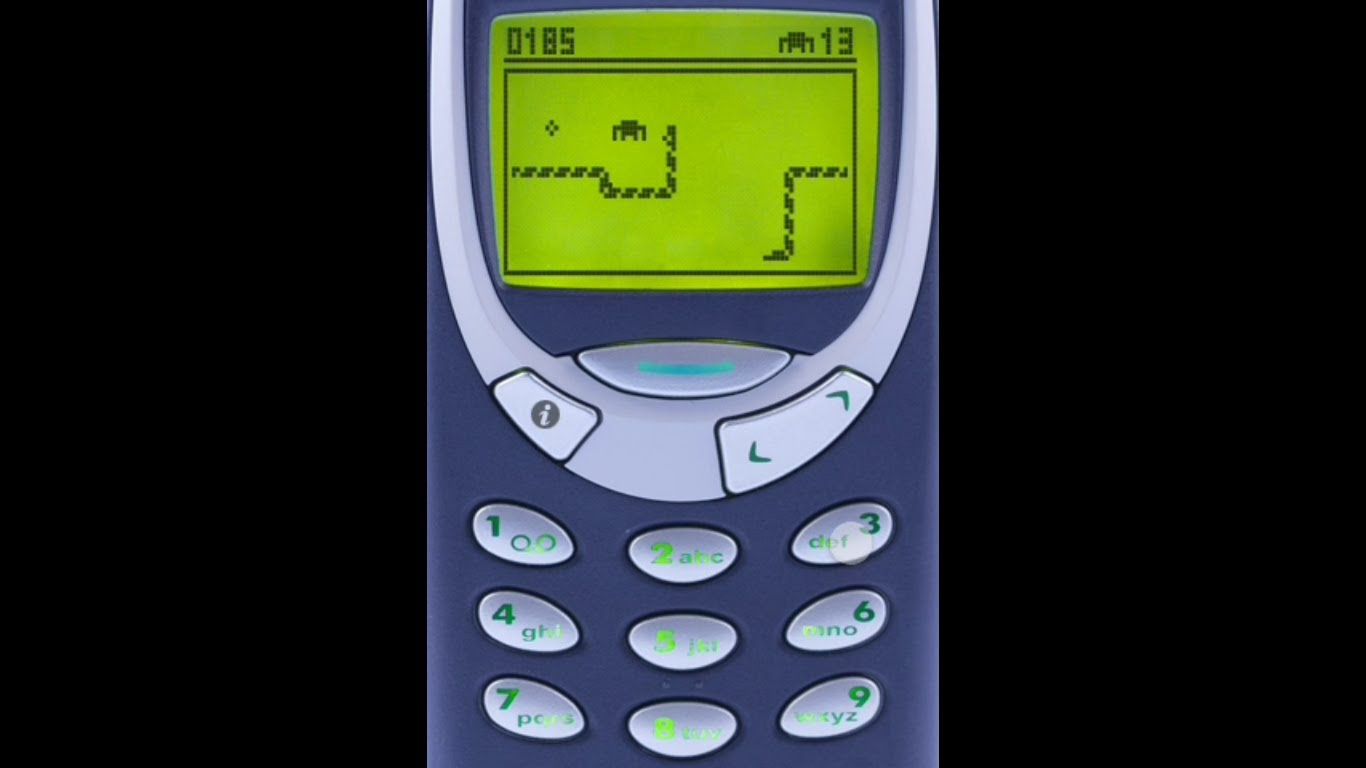
\includegraphics[height=40mm, fbox={\fboxrule} 4mm]{images/introduccion/Nokia_snake.jpg}
\caption{Nokia 3310 con el juego Snake}
\label{fig:Nokia_snake}
\end{figure}

La llegada de Apple a este mercado (figura \ref{fig:Iphone}) supuso una auténtica revolución, ya que cambió el paradigma del teléfono móvil como elemento comunicativo, para convertirlo en algo más.Una estación de trabajo integral llamada a sustituir agendas de trabajo, relojes, reproductores de música, centralitas...\\

%IPHONE
\begin{figure}[hbtp]
\centering
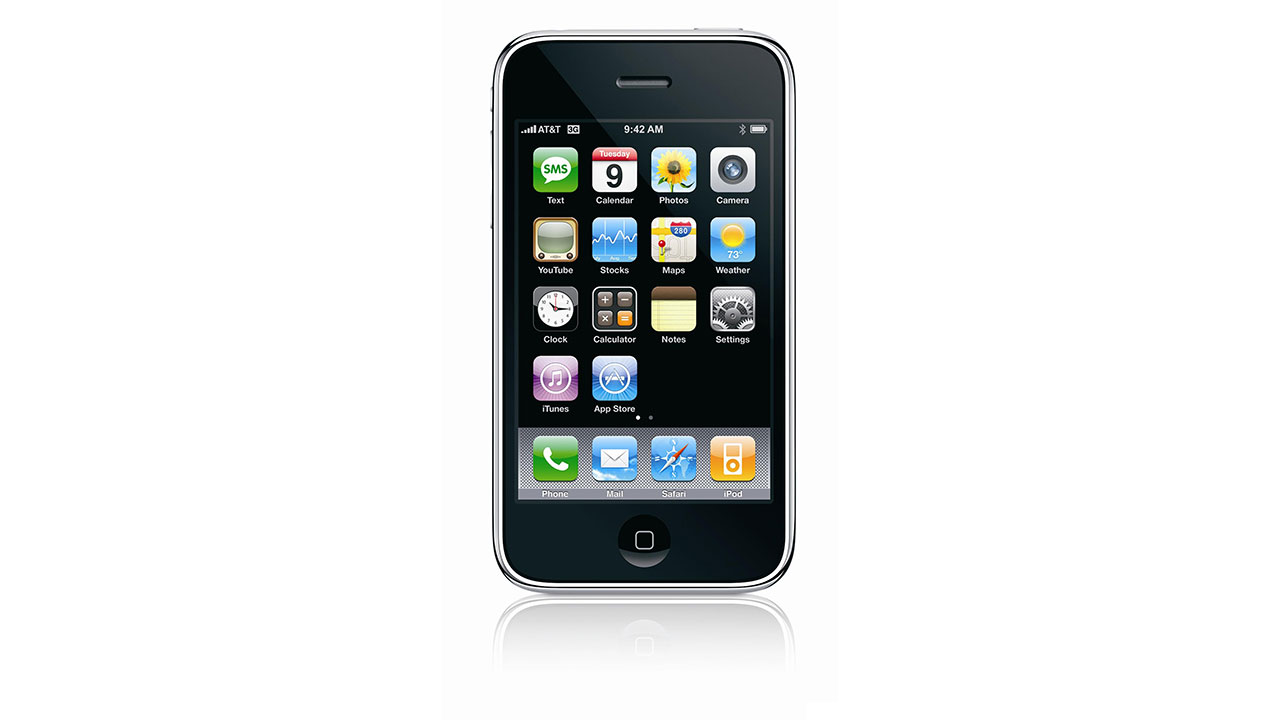
\includegraphics[height=40mm, fbox={\fboxrule} 4mm]{images/introduccion/Iphone1.jpg}
\caption{iPhone 1}
\label{fig:Iphone}
\end{figure}


% INTERNET

Internet, puede ser considerado una de las diez tecnologías que más ha cambiado el mundo, y probablemente la que más rápidamente lo ha conseguido. La aparición de las primeras enciclopedias (figura \ref{fig:Introduccion_enciclopedia}), escritas y editadas con la intención de acercar el conocimiento a las masas, fueron escritas con el propósito de recoger y presentar todo el conocimiento que existía en aquella época. Los enciclopedistas (figura \ref{fig:Introduccion_enciclopedistas}), acorde a las ideas de la ilustración, consideraban que cualquier tipo de mal provenía de la ignorancia, y por tanto la manera de combatir la raíz de los problemas era brindar a las personas la oportunidad de acceder al corpus de conocimientos existente, hasta entonces encerrado en las instituciones académicas y eclesiásticas.

% Imágenes de la primera enciclopedia


\begin{figure}[hbtp]
	\begin{adjustbox}{minipage=\linewidth, fbox}
		\centering
		\subfigure[Árbol de la ciencia de Llull. 1505]{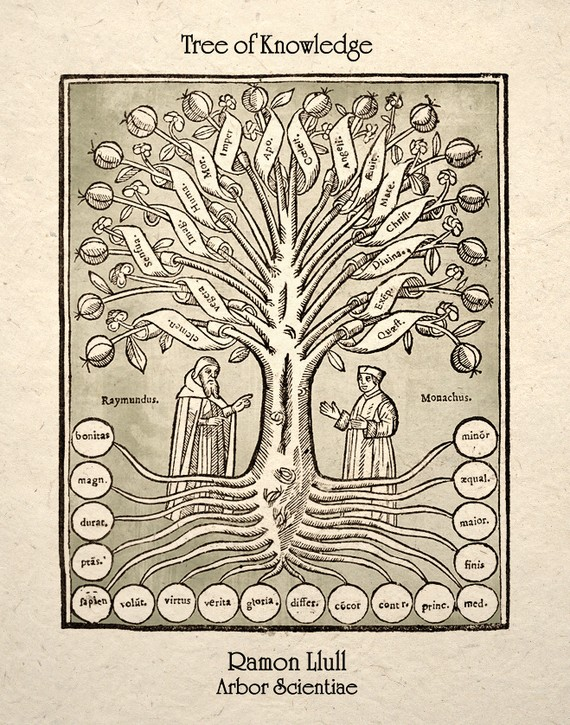
\includegraphics[width=60mm, height=80mm]{./images/introduccion/Arbol_del_conocimiento.jpg}}
		\hspace{10mm}
		\subfigure[Portada de L'Encyclopédie. 1751]{\includegraphics[height=80mm]{./images/introduccion/Enciclopedia_portada.jpg}}
		\vspace{10mm}
		\subfigure[Estructura organizada del conocimiento humano. 1752]{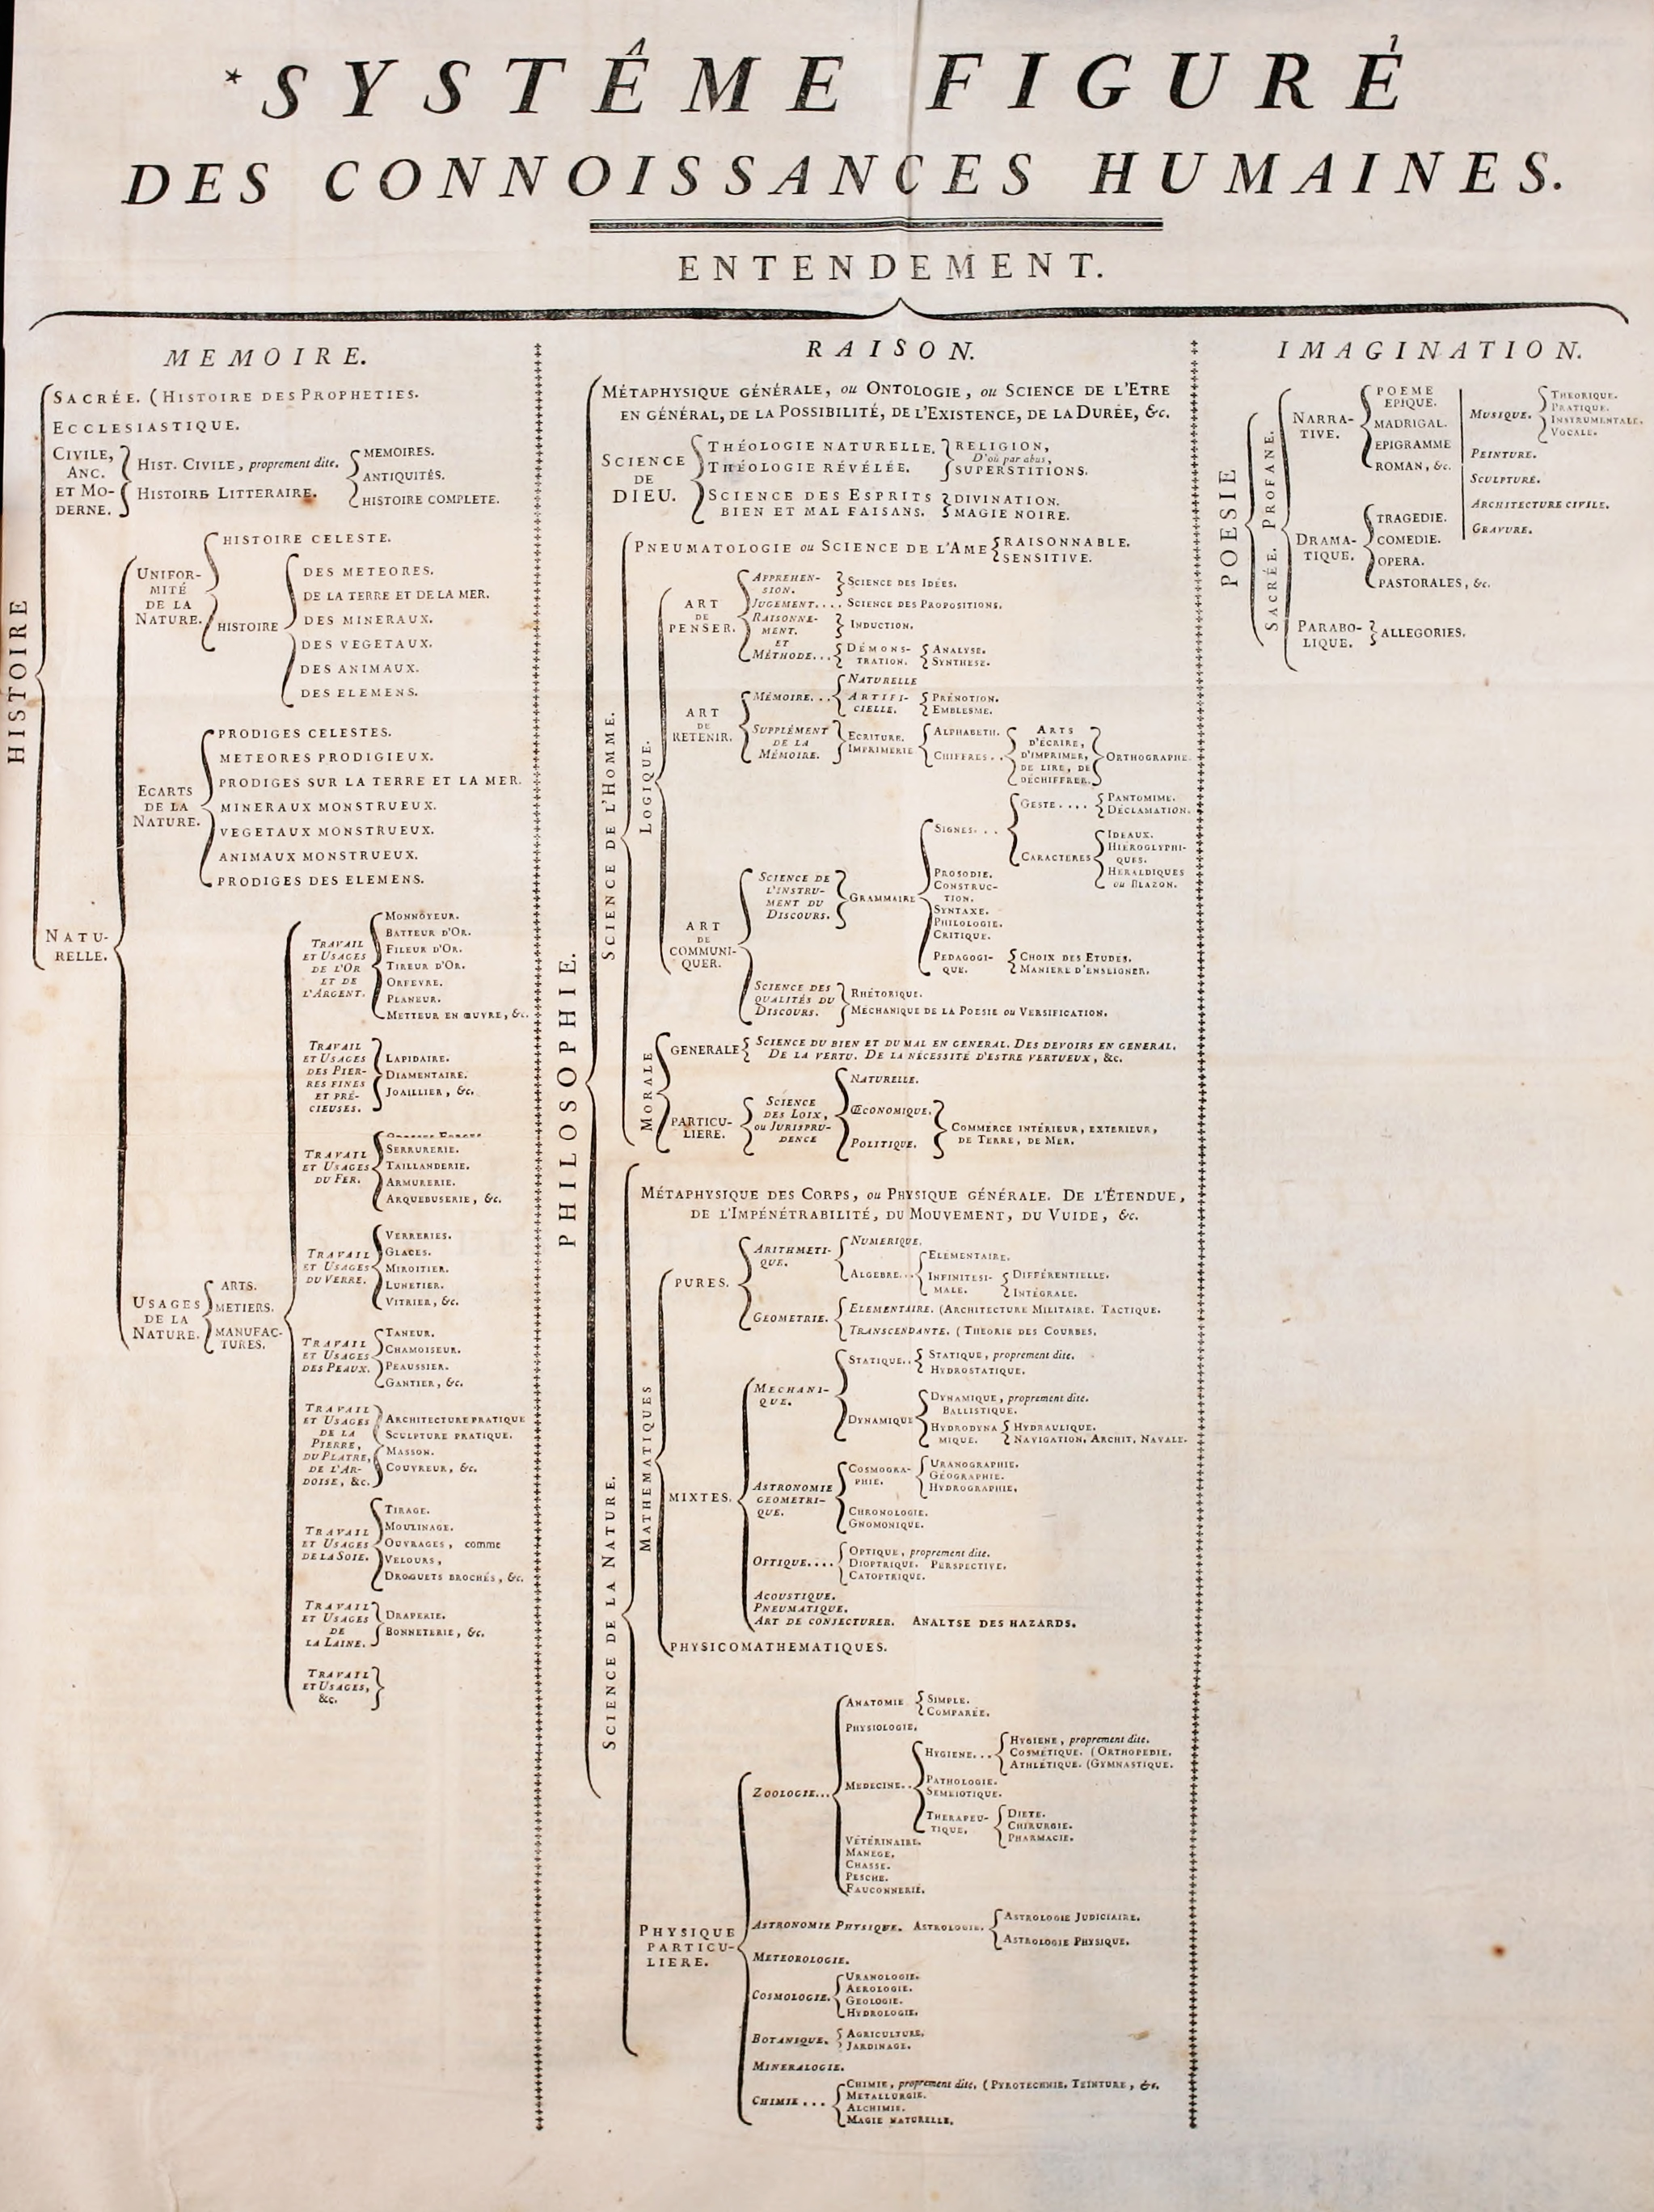
\includegraphics[width=80mm, height=110mm]{./images/introduccion/Conocimiento_humano.jpeg}}
	\end{adjustbox}
	\caption{Árbol de la ciencia de Llull y l'Encyclopédie de Diderot y d'Alembert}
	\label{fig:Introduccion_enciclopedia}
\end{figure}


% FIN imágenes de la primera enciclopedia

% Imágenes enciclopedistas
\begin{figure}[hbtp]
	\begin{adjustbox}{minipage=\linewidth, fbox}
		\centering
		\subfigure[Retrato de Denis Diderot. 1767]{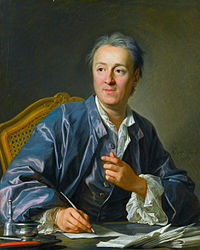
\includegraphics[width=60mm]{./images/introduccion/Diderot}}
		\hspace{20mm}
		\subfigure[Retrato de Jean Le Rond d'Alembert. 1753]{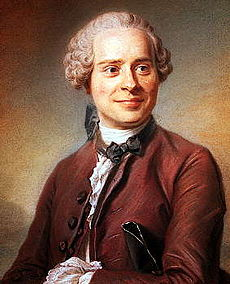
\includegraphics[width=60mm]{images/introduccion/D_Alembert.jpeg}}
		\label{fig:Introduccion_enciclopedistas}
	\end{adjustbox}
\caption{Primeros enciclopedistas}
\end{figure}
% FIN imágenes enciclopedistas

Aunque inicialmente las redes de computadores que finalmente acabarían desembocando en lo que actualmente conocemos como Internet, eran de uso militar, en el año 1983  comienza su andadura \acs{ARPANET} permitiendo el intercambio masivo de datos dando acceso de universidades y centros de investigación (figura \ref{fig:Arpanet}).%http://www.analfatecnicos.net/pregunta.php?id=77

\begin{figure}[hbtp]
\centering
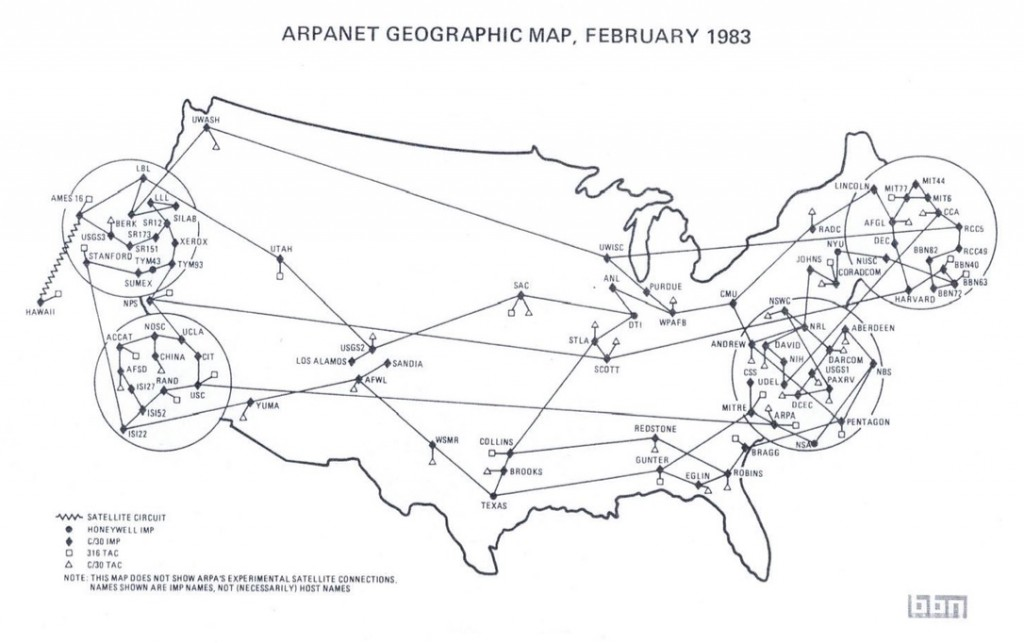
\includegraphics[width=160mm, fbox={\fboxrule} 4mm]{images/introduccion/Mapa_de_Arpanet.jpg}
\caption{Mapa de Arpanet}
\label{fig:Arpanet}
\end{figure}


En el año 2012 existían en internet 634 millones de páginas web. La enciclopedia de Diderot y d'Alembert comprendía un total de 28 volúmenes con 72.999 artículos (figura \ref{fig:Crecimiento_Internet}). %https://es.wikipedia.org/wiki/L%27Encyclop%C3%A9die http://aci.info/2013/10/24/the-history-and-evolution-of-the-internet-media-and-news-in-5-infographics/

\begin{figure}[hbtp]
\centering
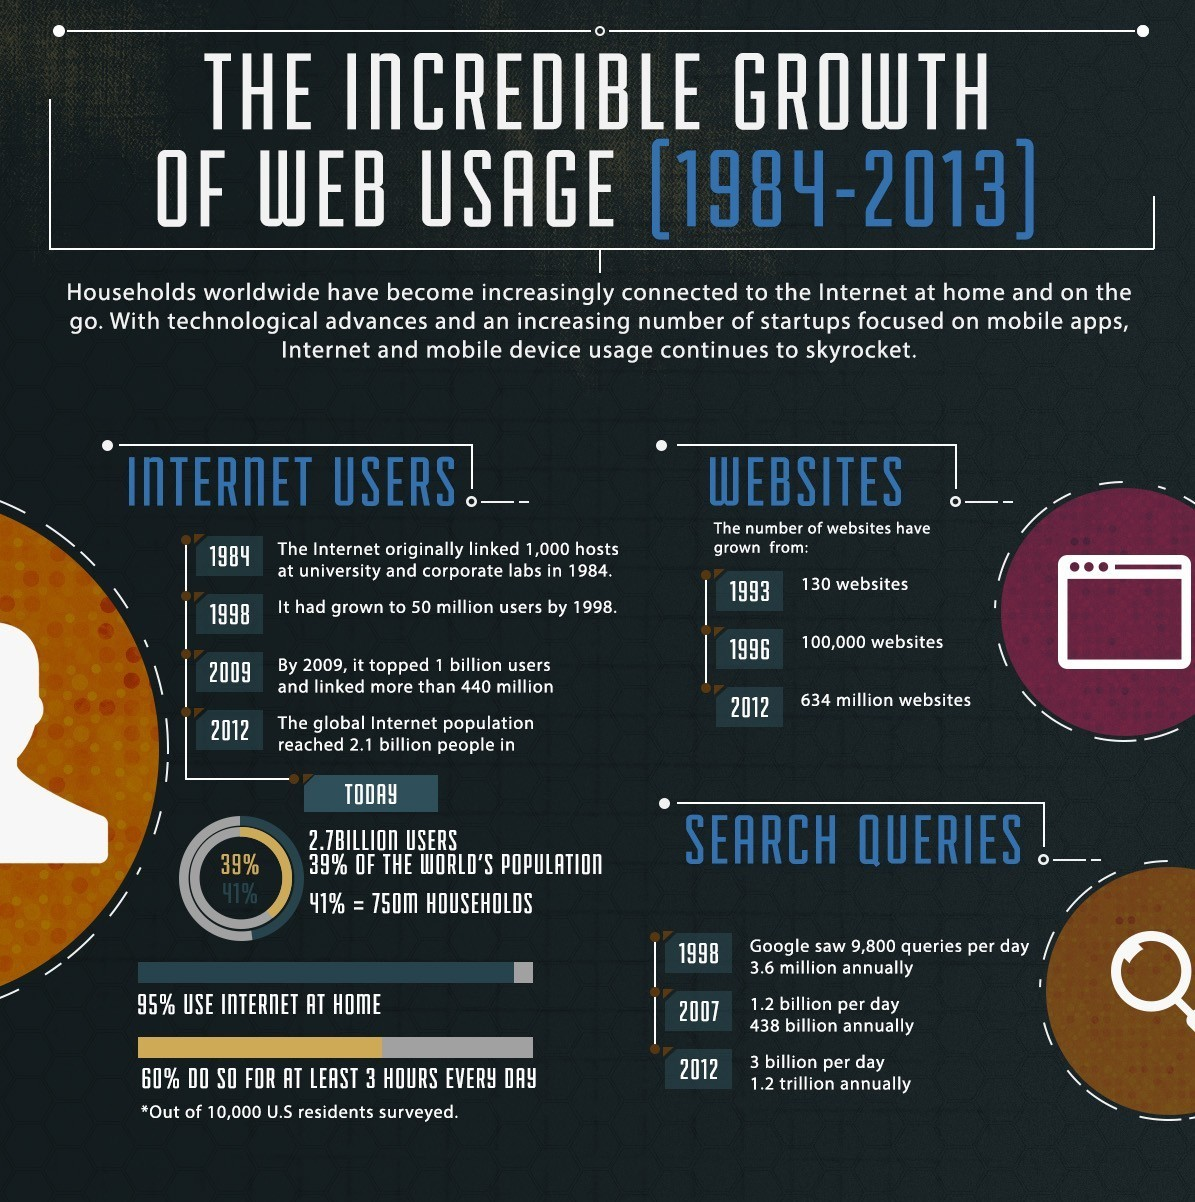
\includegraphics[width=150mm, fbox={\fboxrule} 0pt]{images/introduccion/Grafico_paginas_web.jpg}
\caption{Crecimiento Internet}
\label{fig:Crecimiento_Internet}
\end{figure}


Pero la cantidad disponible de información no es una cuantificación válida de su calidad. El acceso a la información es extremadamente sencillo, pero también lo es la creación de contenidos. De la misma manera que los grandes proyectos enciclopédicos fueron escritos por grandes científicos, matemáticos, ingenieros y filósofos de la época, actualmente cualquier persona con un ordenador puede crear contenido fácilmente y ponerlo a disposición del mundo.

% 


La geolocalización es una faceta omnipresente en la vida diaria actual, es por ello que no resulta extraño que los dispositivos móviles guarden automáticamente la posición en la que se realiza una fotografía o el lugar desde donde se escribe un comentario en una red social. Aunque existen varios proyectos de geolocalización (figura \ref{Logos_satelites}), tales como Galileo, \ac{GLONASS}, \ac{IRNSS} y Beidou, \ac{GPS} es el más conocido, y su nombre se utiliza como sinónimo de cualquier proyecto de posicionamiento por satélite.

\begin{figure}[hbtp]
\centering

\includegraphics[scale=0.75, fbox={\fboxrule} 4mm]{images/introduccion/Sistemas_posicionamiento_satelites.jpg}
\caption{Logotipos de proyectos de geolocalización}
\label{Logos_satelites}
\end{figure}


% PRESENTAR EL PROYECTO

Conociendo estos hechos y teniendo en cuenta que prácticamente todos los modelos de dispositivos móviles del mercado permiten el acceso a internet e incorporan receptores \ac{GPS}, resulta interesante abordar un trabajo dedicado a ahondar en el conocimiento de temas tan extendidos como la geolocalización, los dispositivos móviles y el desarrollo web.

Es un hecho cotidiano olvidar el lugar de aparcamiento del vehículo, la dirección exacta del alojamiento hotelero y un sinfín de ejemplos similares. Desarrollar una aplicación que permita guardar, recuperar y mostrar el camino hacia una dirección exacta, resulta una opción interesante.

La idea general, consiste en un sistema que permita al usuario almacenar de forma sencilla y rápida una posición geográfica para más tarde permitir recuperarla. Aunque los usos pueden ser variados, el desarrollo se centrará en el almacenamiento de la posición de aparcamiento de vehículos.Se permitirá que varios usuarios accedan a una misma posición almacenada, bien para mostrarla, bien para modificarla, ateniéndonos a la posibilidad de que varios usuarios pueden compartir el uso o propiedad de un mismo vehículo.

\section{Estructura del documento}

\begin{definitionlist}
	\item[Capítulo \ref{chap:introduccion}: \nameref{chap:introduccion}.] Breve introducción acerca del tema a tratar durante el desarrollo del \ac{TFG} y presentación superficial de la herramienta.
	\item[Capítulo \ref{chap:objetivos}: \nameref{chap:objetivos}.] Objetivos principal y parciales que se deben cumplirse para dar por finalizado el desarrollo.
	\item[Capítulo \ref{chap:antecedentes}: \nameref{chap:antecedentes}.] Presentación de los temas circundantes a la herramienta a desarrollar, estado del arte y aplicaciones con similitudes a la herramienta presentada en el \ac{TFG}.
	\item[Capítulo \ref{chap:metodo}: \nameref{chap:metodo}.] Explicación de la metodología utilizada para la consecución de los objetivos expuestos en el capítulo 2. Presentación de las herramientas utilizadas a lo lardo del desarrollo.
	\item[Capítulo \ref{chap:resultados}: \nameref{chap:resultados}.] Exposición detallada de los resultados obtenidos durante el desarrollo.
	\item[Capítulo \ref{chap:conclusiones}: \nameref{chap:conclusiones}.] Propuestas de mejora para la herramienta, conclusión final y valoración personal.
	\item[Anexo \ref{chap:manual}: \nameref{chap:manual}.] Manual de usuario.
	\item[Anexo \ref{chap:acronimos}: \nameref{chap:acronimos}.] Listado de los acrónimos utilizados en la presente memoria.
	\item[Anexo \ref{chap:source}: \nameref{chap:source}.] Localización donde encontrar el código fuente relativo al presente \ac{TFG}.

	
%	\item[Capítulo \ref{chap:antecedentes}: \nameref{chap:antecedentes}] Explica herramientas y aspectos básicos de edición con \LaTeX.
%	\item[Capítulo \ref{chap:objetivos}: \nameref{chap:objetivos}] Finalidad y justificación (con todo detalle) del presente documento.

\end{definitionlist}



% Local Variables:
%  coding: utf-8
%  mode: latex
%  mode: flyspell
%  ispell-local-dictionary: "castellano8"
% End:

\chapter{Objetivos}
\label{chap:objetivos}

\noindent
Para este capítulo, la normativa indica:

«Concretar y exponer el problema a resolver describiendo el entorno de trabajo,
la situación y detalladamente qué se pretende obtener. Limitaciones y
condicionantes a considerar para la resolución del problema (lenguaje de
construcción, equipo físico, equipo lógico de base y de apoyo, etc.). Si se
considera necesario, esta sección puede titularse ``Objetivos e hipótesis de
trabajo''. En este caso, se añadirán las hipótesis de trabajo que el alumno, con
su TFG, pretende demostrar».

\section{Objetivo general}

El hito final que se pretende lograr, destacando el problema específico que
resuelve o la funcionalidad que aporta la aplicación o sistema desarrollado.


\section{Objetivos específicos}

Los objetivos específicos son las partes independientes del proyecto que tienen
valor por si mismas.

Por ejemplo, si el objetivo general fuera destruir una flota enemiga, los
objetivos específicos podrían ser: hundir el portaaviones, inutilizar las
torretas de los destructores, eliminar los cazas enemigos, etc.

Los objetivos específicos no son tareas; análisis, diseño, etc. no tienen valor
intrínseco para el cliente, si por ejemplo el proyecto se cancela en la fase de
diseño no se le entrega nada de valor al cliente, luego no se cubre ningún
objetivo.

No se deben confundir los objetivos del proyecto con los objetivos del
alumno. Indicar como objetivo que el alumno va a aprender o a estudiar
determinada disciplina o herramienta no aporta nada al cliente. Deben ser
entregables que el cliente puede valorar y por los que estaría dispuesto
a pagar. Resumiendo, son \textbf{objetivos}, no subjetivos.

\subsection{Objetivo 1}

\subsection{Objetivo 2}

\subsection{Objetivo 3}


% Local Variables:
%  coding: utf-8
%  mode: latex
%  mode: flyspell
%  ispell-local-dictionary: "castellano8"
% End:

\chapter{Antecedentes}
\label{chap:antecedentes}

\drop{E}{n} este capítulo se muestra el trabajo de documentación e investigación previa a la realización del presente \ac{TFG}. En primer lugar se abordarán los sistemas de posicionamiento, su historia y el desarrollo del gps\footnote{Debido al extendido uso de la denominación \textit{GPS} como sinónimo de los \ac{GNSS}, se usará de este modo. Para referirse al sistema de posicionamiento propiedad del gobierno de los Estados Unidos \acf{GPS} se utilizará el acrónimo en mayúsculas} 

y los antecedentes de los \ac{SIG}, más tarde se comentarán algunos aspectos relevantes de la web y de las tecnologías móviles. Para terminar, se enumerarán algunas aplicaciones similares que podemos encontrar actualmente en el mercado.

\section{Localización geográfica y \acf{SIG}}

%HISTORIA DEL GPS
Los \ac{GNSS} permiten conocer en tiempo real la posición de un objeto cualquiera en la superficie terrestre.

Según Scott Gleason y Demoz Gebre-Egziabher \cite{Glea09} podríamos definir la navegación como:

	\vspace{5mm}
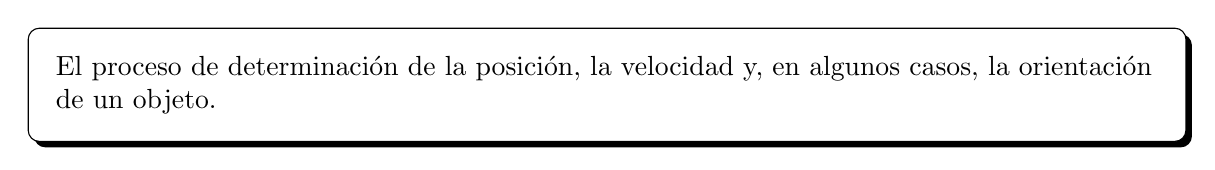
\begin{tikzpicture}
	\node[shadowBox] {El proceso de determinación de la posición, la velocidad y, en algunos casos, la orientación de un objeto.};
\end{tikzpicture}
	\vspace{5mm}

Por tanto, un \ac{GNSS} consiste en una constelación de satélites que permiten determinar con precisión las coordenadas geográficas y la altitud de un punto dado en cualquier punto de la superficie terrestre.

El inicio de este tipo de sistemas podríamos encontrarlo en los primeros marinos. La decisión de alejarse de las rutas que transcurrían a lo largo de la línea de visión de la costa, con la intención de reducir el tiempo, los costes derivados de los viajes y la posibilidad de encontrar nuevos mercados, planteó un nuevo reto tecnológico consistente en conocer con exactitud la localización en la que se encontraban.
La primera solución vino de la mano de un gran conocimiento de la bóveda celeste y la posición de las estrellas. Usando instrumentos como el astrolabio y el sextante (ver figura \ref{fig:sextante_astrolabio}), se podía calcular con asombrosa exactitud la posición.

\begin{figure}[h!btp]
	\begin{adjustbox}{minipage=\linewidth, fbox}
		\centering
		\subfigure[Sextante]{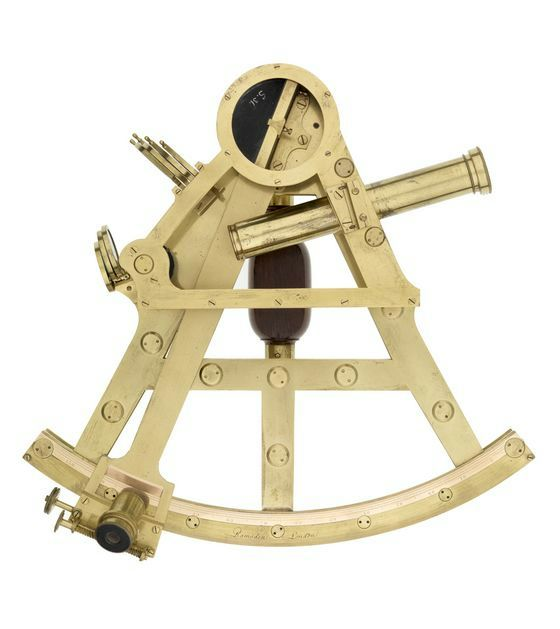
\includegraphics[width=60mm, height=80mm]{./images/03-antecedentes/04-sextante.png}}
		\hspace{10mm}
		\subfigure[Astrolabio]{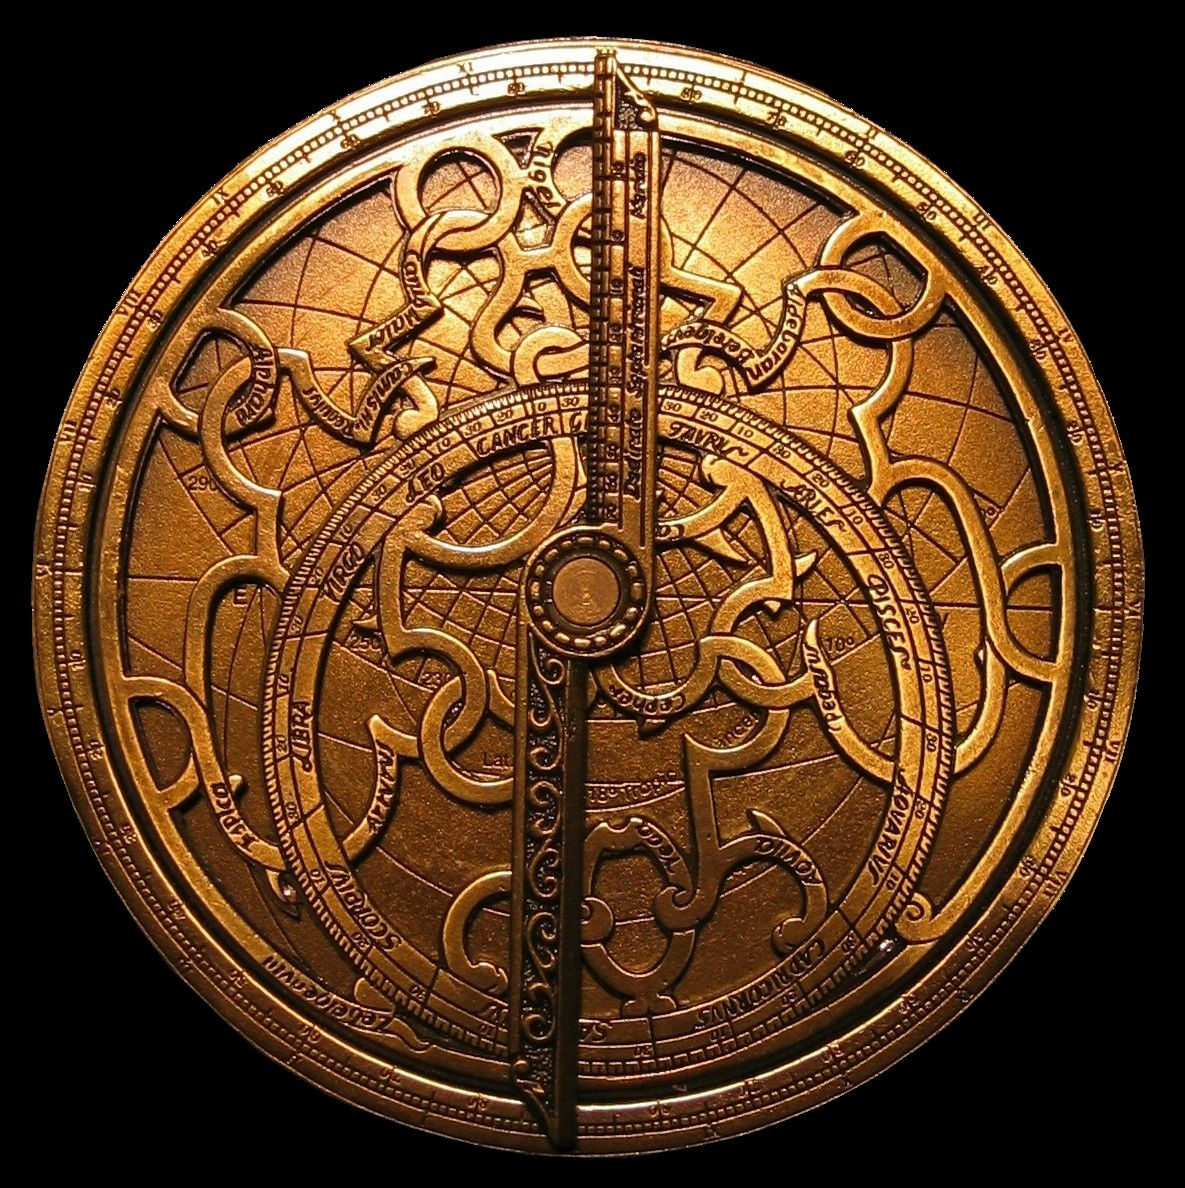
\includegraphics[height=80mm]{./images/03-antecedentes/05-astrolabio.png}}
	\end{adjustbox}
	\caption{Primeros instrumentos de navegación}
	\label{fig:sextante_astrolabio}
\end{figure}

Hasta tiempos recientes (segunda mitad del S. XX), con la irrupción del posicionamiento satelital, este era el método usado para conocer la ubicación en la que se encontraban.
Los primeros prototipos del gps se desarrollan a principios del S. XX, coincidiendo con los comienzos de la automoción, aspecto este último que ha dado la gran fama a esta tecnología.
El primer gps data de 1909, que consistía en un odómetro que giraba un mapa indicando los hitos más importantes que se podían encontrar en el punto kilométrico en el que estabas.
Este primer prototipo se llamaba \textit{Jones Live Map} (ver figura \ref{fig:jones_live_map}), cada mapa era válido para unos 160 km y después había que cambiarlo por el siguiente mapa. Este primer intento dejó de fabricarse en los años 20, cuando las carreteras estaban correctamente señalizadas \cite{GPS12}.

\begin{figure}[h!btp]
\centering
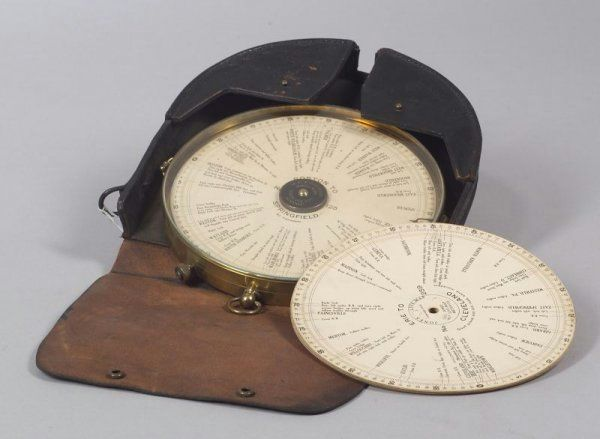
\includegraphics[scale=0.5, fbox={\fboxrule} 4mm]{images/03-antecedentes/06-jones_live_map.png}
\caption{Jones Live Map}
\label{fig:jones_live_map}
\end{figure}

También en la década de los veinte, hizo su aparición el \textit{Plus Fours Routefinder} (ver figura \ref{fig:plus_fours_routefinder}), consistente en un pequeño reloj de muñeca con una serie de papiros con la información de la ruta que debían ir desenrollándose de forma manual para ir viendo las indicaciones \cite{Plus14}.

\begin{figure}[h!btp]
\centering
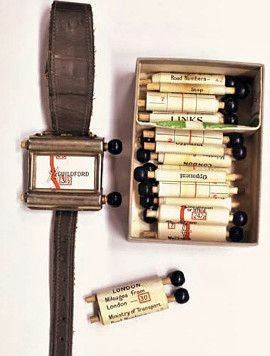
\includegraphics[scale=0.5, fbox={\fboxrule} 4mm]{images/03-antecedentes/07-plus_fours_routefinder.png}
\caption{Plus Fours Routefinder}
\label{fig:plus_fours_routefinder}
\end{figure}

Otro de los padres del gps moderno es el llamado \textit{Iter Avto} (ver figura \ref{fig:iter_avto}), consistente en un mapa enrollado conectado al velocímetro del coche para sincronizarlo. La dos grandes ventajas con respecto al \textit{Plus Fours Routefinder}, consistía en que se instalaba sobre el salpicadero del coche y mostraba de forma gráfica la posición. Su inconveniente, cualquier desviación de la ruta era completamente indetectable \cite{Parra13}.

\begin{figure}[h!btp]
\centering
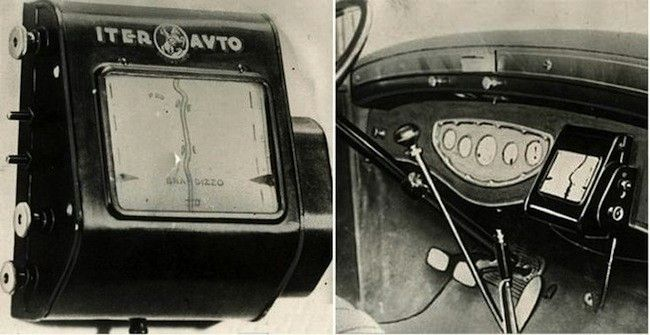
\includegraphics[scale=0.5, fbox={\fboxrule} 4mm]{images/03-antecedentes/08-iter_avto.png}
\caption{Iter Avto}
\label{fig:iter_avto}
\end{figure}

Durante la segunda guerra mundial, la \ac{RAF} desarrolló un sistema de
posicionamiento para sus bombarderos consistente en tres estaciones de radar que localizaban
con precisión al avión \cite{Ori13}.
Los verdaderos orígenes de los gps como sistema de navegación satelital se remontan a 1957 con
el programa \textit{TRANSIT}. Por un lado la marina de los estados unidos inicia el programa \textit{Polaris},
que consiste en el despliegue de misiles transcontinentales suboceánicos. Alcanzar los objetivos
con los misiles dependía de la capacidad de determinar con precisión la posición de los
submarinos en cualquier punto de la superficie terrestre. Por otro lado, la universidad Johns
Hopking de Maryland, consigue determinar con precisión la órbita del \textit{Sputnik 1} a partir del
desplazamiento Doppler sufrido por la señal que emitía y el conocimiento preciso de la posición
del receptor. Con estos elementos, invertir los términos del problema resultó relativamente
sencillo, esto es, conociendo la posición de un satélite de forma precisa, es posible determinar
la de un receptor situado en el submarino de posición desconocida midiendo el desplazamiento
Doppler sufrido por la señal emitida del satélite.

El sistema \textit{TRANSIT} entró en funcionamiento en 1964 con el lanzamiento de 10 satélites y se mantuvo en servicio
hasta 1996. En 1967 se permitió su uso civil. El error típico de este sistema era de unos 250
metros, por lo que resultaba muy útil para la navegación de aviones, barcos y submarinos, pero
por razones obvias (precisión y tamaño de los receptores) aún estaban lejos de los sistemas de
navegación personal actuales.

La Unión Soviética había desarrollado casi al mismo tiempo, un sistema muy parecido con
idénticas prestaciones, el \textit{TSICADA}, lo que resultaba inadmisible para los norteamericanos en el
contexto de la guerra fría, por lo que comenzó a desarrollarse lo que posteriormente sería el
\ac{GPS} \cite{Pala10}.
El \textit{NAVSTAR-GPS} nació en 1973 para uso exclusivamente militar, con una constelación de 24
satélites en órbitas inclinadas de 12 horas, lo que se traducía en que cualquier receptor en el
mundo tendría en su horizonte visible al menos 5 satélites disponibles en todo momento. El
TRANSIT, no sólo no podía garantizar esto, debido a que sus satélites eran de órbita baja, si no
que con sus 6 satélites, algunos receptores podían estar varias horas esperando señal. El primer
satélite se puso en órbita en 1978. La precisión de este nuevo sistema era de 1 metro y podía
ser incorporado en misiles, bombas inteligentes, vehículos, etc. Debido a su consideración de
recurso de gran valor estratégico, su uso estaba limitado al ámbito estrictamente militar.
El 31 de agosto de 1983 tuvo lugar uno de los incidentes internacionales más graves de la
guerra fría, que a la postre resultaría decisivo para el uso actual del \ac{GPS}, el derribo del vuelo de
\textit{Korean Airlines KAL007} por parte de la \ac{URSS} \cite{Kore15}.

El citado vuelo, usando los sistemas de navegación tradicionales disponibles en aquella época, y
usando el piloto automático, invadió en dos ocasiones el espacio aéreo de la Unión Soviética,
que acabó interceptándolo mediante dos cazas militares y derribándole con un ataque con
misiles, matando al pasaje y la tripulación completa, con un resultado de 269 fallecidos.
La respuesta internacional no se hizo esperar, y el entonces presidente de \ac{USA}, Ronald Reagan,
anunció que el sistema \ac{GPS} estaría disponible para propósitos civiles una vez finalizase el
proyecto, con la intención de que no se volvieran a repetir incidentes similares.
Para evitar que sus enemigos pudieran hacer uso de esta nueva tecnología para construir
misiles de precisión con los que atacarlos, el Departamento de Defensa de \ac{EE.UU.} impuso una
serie de restricciones en la precisión de los receptores, de manera que el error en el
posicionamiento fuera mayor que el de los disponibles para uso militar. Por ello los receptores de gps de uso
civil eran incapaces de mostrar una resolución menor de 20 metros.
Durante la primera guerra del golfo, en 1991, se desarrolló una mejora en la precisión del \ac{GPS}
llamada, \ac{GPS} Diferencial, que conseguía precisiones de entre 1 y 3 metros de exactitud.

\subsection{Funcionamiento de los gps}

La base sobre la que se asienta el funcionamiento del posicionamiento mediante satélites consiste en que sea cual sea nuestra localización en la corteza terrestre, siempre estaremos a la vista de al menos cuatro satélites distintos.

Cada uno de estos satélites transmite información acerca de su localización que será utilizada por nuestro receptor para calcular la distancia a la que se encuentran, en función del tiempo que tardan las señales en llegar.
Conociendo la distancia a la que se encuentran, como mínimo, tres satélites, es posible conocer con un cierto grado de aproximación la zona en la cual debemos estar posicionados. Este proceso de localizacion se conoce como triangulación.

Si estamos al alcance de un único satélite, la posible zona en la que nos encontraremos será todo el área de influencia del mismo. En el caso de utilizar dos satélites, la zona en la que podríamos encontrarnos sería la superficie de la intersección de las dos esferas imaginarias creadas con centro cada uno de los satélites y radio la distancia a nuestra posición.

En el caso de utilizar tres satélites, que como hemos comentado anteriormente es el mínimo necesario, la posible localización se ve reducida a dos puntos. Para conocer con precisión cual de esos dos puntos es el correcto haría falta un cuarto satélite, pero en términos generales, uno de ellos no estará ubicado en la corteza terrestre, por lo que podrá descartase y conocer de esta manera nuestra localización (ver figura \ref{fig:triangulacion-satelital}).

\begin{figure}[h!btp]
\centering
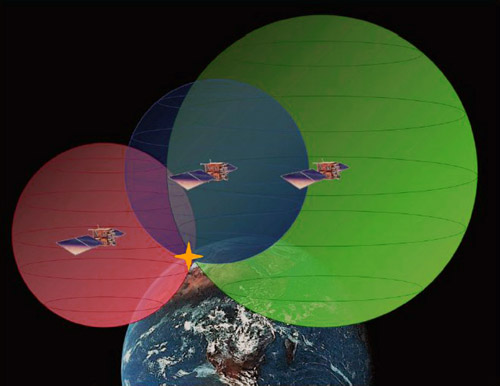
\includegraphics[scale=0.5, fbox={\fboxrule} 0mm]{images/03-antecedentes/31-funcionamiento_gps.jpg}
\caption{Triangulacion satelital}
\label{fig:triangulacion-satelital}
\end{figure}

Debido a razones de obvias de estrategia militar, la precisión dada por los satélites \ac{GPS} incluía un cierto grado de error aleatorio llamado \textit{disponibilidad selectiva}. Este error fue eliminado el 2 de mayo del año 2000. Habitualmente la precisión para usos civiles se veía limitada a 100 metros \cite{Corr00}.

\subsection{Cartografía y \acs{SIG} \protect\footnote{La labor de documentación está basada en: \cite{Diaz15}.} }

Antes de la aparición de la historia, esto es, antes de la constatación escrita de los acontecimientos, se produjo la aparición de los mapas. Estos estaban realizados con la intención de establecer distancias, recorridos y localizaciones de elementos de cierta importacia.

El mapa más antiguo del que se tiene noticia proviene de la antigua Babilonia y está fechado alrededor de 4500 años a.C. Actualmente está conservado en Museo Británico (ver figura \ref{fig:mapa-babilonio}).

\begin{figure}[h!btp]
\centering
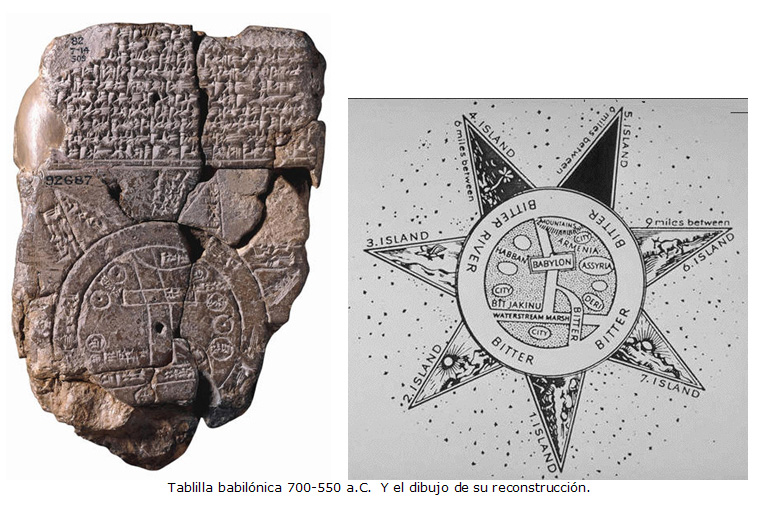
\includegraphics[scale=0.5, fbox={\fboxrule} 0mm]{images/03-antecedentes/32-mapa_babilonio.jpg}
\caption{Tablilla babilónica y reconstrucción}
\label{fig:mapa-babilonio}
\end{figure}

La antigua Grecia fue quien colocó las bases para la cartografía actual, aportando grandes conocimientos geométricos, matemático geográficos y  astronómicos. Los cartógrafos griegos, que admitían la forma esférica de la tierra, fueron los iniciadores del sistema de localización geográfica, es decir, las latitudes y longitudes, hicieron las primeras proyecciones \cite{Schl07} y dieron una cifra bastante aproximada del tamaño de nuestro planeta \cite{Aup09}.

Prácticamente todo lo que conocemos de la cartografía de este tiempo se debe a los escritos de Herodoto y Estrabón que mencionan a Anaximándro de Mileto como el realizador de un mapa completo de la tierra incorporando mares y ríos \cite{Kap10}. Pero de entre todos los personajes de la antigua gracia, fue Claudio Ptolomeo el más importante para el campo de la cartografía con su obra \textit{Geographia} en la que se puede apreciar un mapamundo que abarca desde las islas Canarias por el oeste hasta China por el este (ver figura \ref{fig:mapa-ptolomeo}). Debido a que en este mapa aparecen las latitudes, el ecuador la escala y está orientado al norte, es posible apreciar las bases de las cartas de navegación modernas.

\begin{figure}[h!btp]
\centering
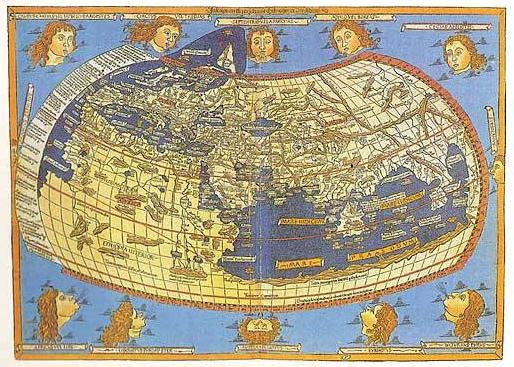
\includegraphics[width=120mm, fbox={\fboxrule} 0mm]{images/03-antecedentes/33-mapa_ptolomeo.jpg}
\caption{Mapa Ptolemáico}
\label{fig:mapa-ptolomeo}
\end{figure}

Durante la era romana se sufrió un retroceso en la cartografía, que no volvería a los niveles griegos hasta el siglo XVI, ya que estaban más interesados en la realización de mapas prácticos de fines militares, administrativos y comerciales que en plasmar la realidad sobre el papel.

Durante la edad media, se pierde el concepto de esfera en los mapas y se representa el mundo ateniéndose más a conceptos místicos y religiosos que a la propia realidad. Normalmente aparece Jerusalén en el centro del mapa, como ejemplo en la figura \ref{fig:mapa-beato-liebana} se puede observar el mapamundi incluido de Beato de Liébana.

\begin{figure}[h!btp]
\centering
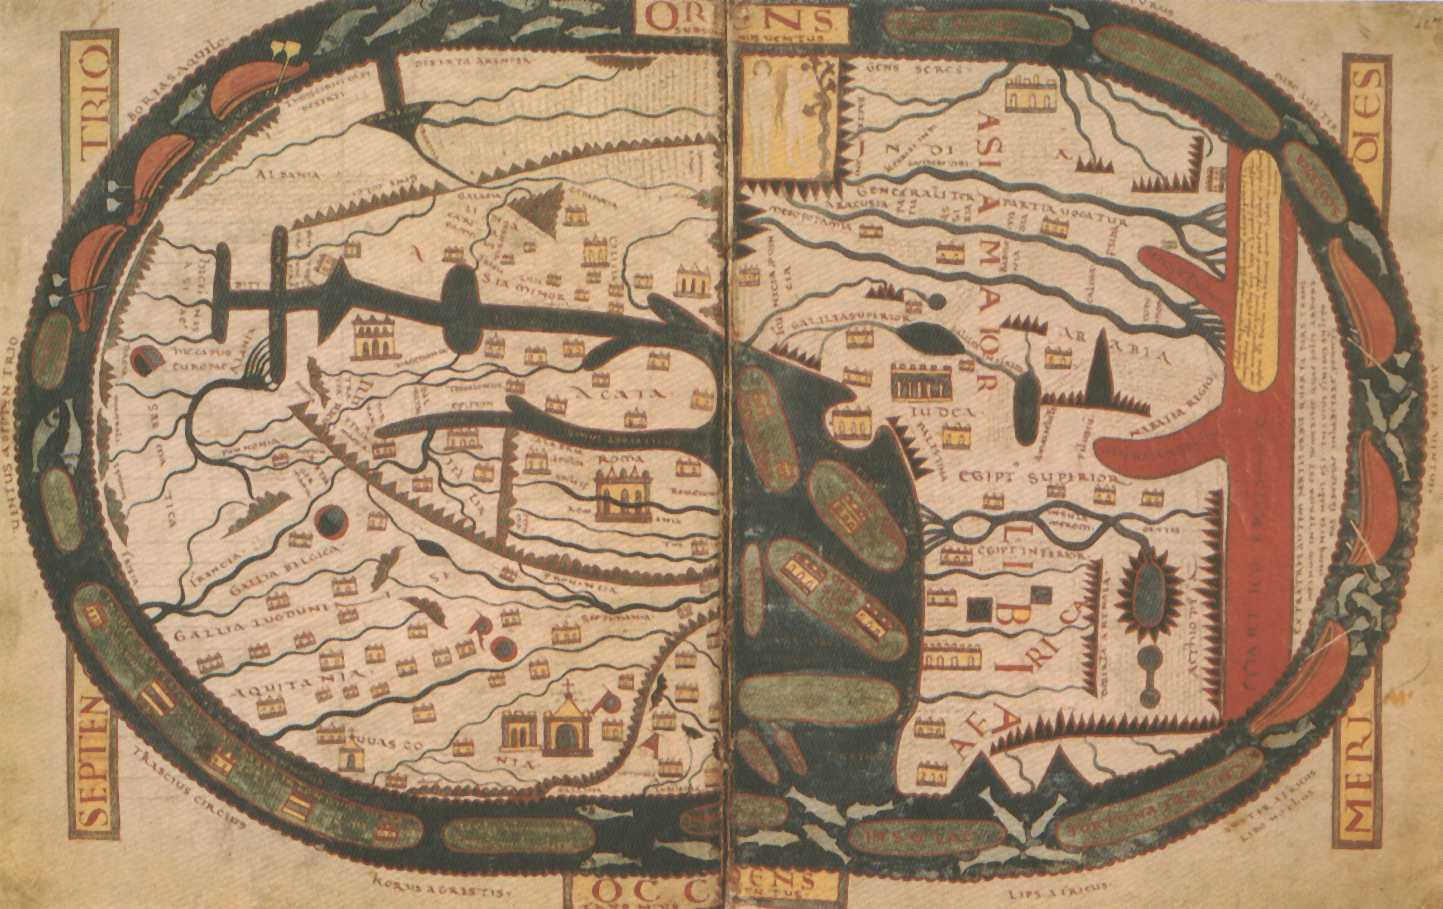
\includegraphics[width=160mm, fbox={\fboxrule} 0mm]{images/03-antecedentes/34-mapa_beato_liebana.jpg}
\caption{Mapamundi de Beato de Liébana}
\label{fig:mapa-beato-liebana}
\end{figure}

En el año 1154, Al Idrisi, cartógrafo ceutí, presenta un mapa alejado de las convenciones europeas existentes en la época y más cercanos a los planteamientos griegos. En su mapa se puede observar con gran detalle los perfiles de Europa, norte de Africa y gran parte de Asia, aunque está orientado hacia el sur, en lugar de la orientación norte a la que estamos acostumbrados (ver figura \ref{fig:mapa-al-idrisi}).

\begin{figure}[h!btp]
\centering
\includegraphics[width=160mm, fbox={\fboxrule} 0mm]{images/03-antecedentes/35-mapa_al_idrisi.jpg}
\caption{Mapamundi de Abu Abd Allah Muhammad al-Idrisi.1154}
\label{fig:mapa-al-idrisi}
\end{figure}

A mediados del siglo XV da comienzo la cartografía moderna como consecuencia de la recuperación de los escritos de Ptolomeo, la invención de la imprenta y la posibilidad de divulgar los mapas con facilidad y los grandes avances técnicos respecto a la brújula y las embarcaciones, que permitían hacer viajes más largos, para lo que necesitaban mejores cartas de navegación.

En el año 1500 aparece el mapa de Juan de la Cosa, y aunque no existe consenso al respecto, la mayor parte de los autores consideran que este es el primer mapa en que aparece América \cite{Verl06}, aunque hay que esperar al año 1507 para poder ver el nuevo continente con su nombre, propuesto por Américo Vespucio, en el mapa de Martin Waldseemüller (ver figura \ref{fig:mapas-america}).

\begin{figure}[h!btp]
	\begin{adjustbox}{minipage=\linewidth, fbox}
		\centering
		\subfigure[Mapamundi de Juan de la Cosa. 1500]{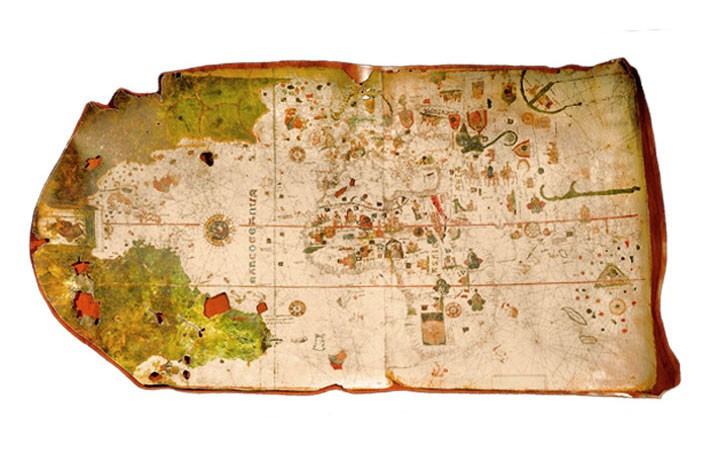
\includegraphics[scale=0.5]{./images/03-antecedentes/36-mapa_juan_de_la_cosa.jpg}}
		\hspace{10mm}
		\subfigure[Mapamundi de Martin Waldseemüller. 1507]{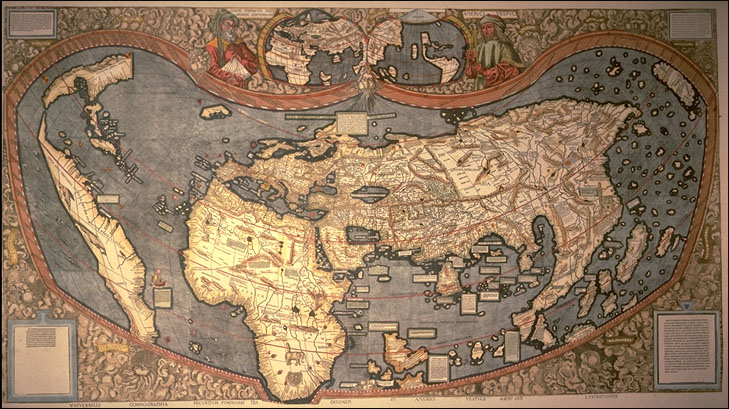
\includegraphics[height=80mm]{./images/03-antecedentes/37-mapa_martin_waldseemuller.jpg}}
	\end{adjustbox}
	\caption{Primeros mapas de América}
	\label{fig:mapas-america}
\end{figure}

Ya en el siglo XX, el desarrollo de la fotografía y la aviación, en el contexto de la Gran Guerra y sobre todo durante la Segunda Guerra Mundial, permitió una gran revolución cartográfica. Siendo conscientes de la gran ventaja militar que suponía el profundo conocimiento del terreno, empiezan a desarrollarse grandes proyectos en este sentido, que culminarán durante la segunda mitad del siglo, en la cartografia de precisión mediante satélites \cite{Lind06}.

Debido a que el término \ac{SIG} engloba la integración de muy diversas áreas,no existe una única definición totalmente consensuada \cite{Chr97}. La definición aportada por el \ac{NCGIA} resulta ampliamente aceptada:

\vspace{5mm}
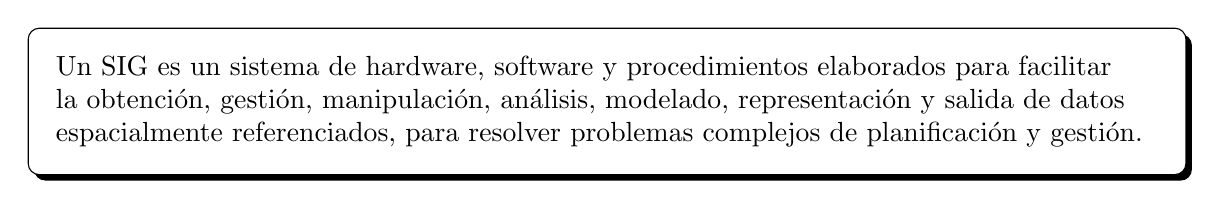
\begin{tikzpicture}
	\node[shadowBox] {
	Un SIG es un sistema de hardware, software y procedimientos elaborados para facilitar la obtención, gestión, manipulación, análisis, modelado, representación y salida de datos espacialmente referenciados, para resolver problemas complejos de planificación y gestión.};
\end{tikzpicture}
\vspace{5mm}

Uno de los elementos relevantes de los \ac{SIG} son la asociación de información a una imagen concreta y una de las primeras muestras de esto lo podemos encontrar en el Londres victoriano de mediados del siglo XIX. En el año 1854, el doctor John Snow (ver figura \ref{fig:john_snow}) utilizó un mapa del Soho londinense para ubicar los casos de un brote de cólera (ver figura \ref{fig:cholera_map}). Con la ayuda de los registros del hospital de Middlesex y de Henry Whitehead, párroco local, recogió las defunciones producidas mediante una fina línea de color negro que se apilaban unas sobre otras a medida que se producían las muertes, consiguiendo el efecto de asociación de información a imagen comentado en el párrafo anterior \cite{Cai11}.

Este ejemplo temprano, combinado con la geolocalización nos permite identificar las líneas base de representación de lo que será el presente \ac{TFG}.

\begin{figure}[h!btp]
\centering
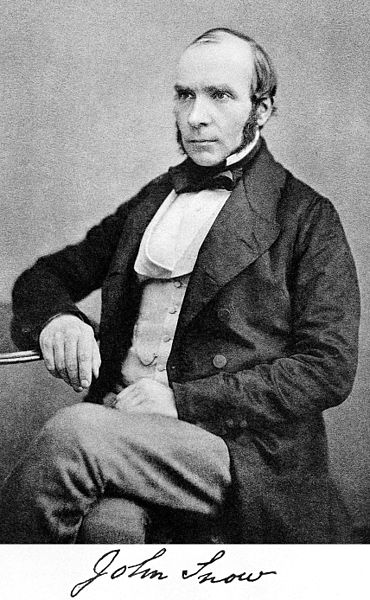
\includegraphics[scale=1, fbox={\fboxrule} 0mm]{images/03-antecedentes/02-john_snow.jpg}
\caption{Doctor Sir John Snow}
\label{fig:john_snow}
\end{figure}

\begin{figure}[h!btp]
\centering
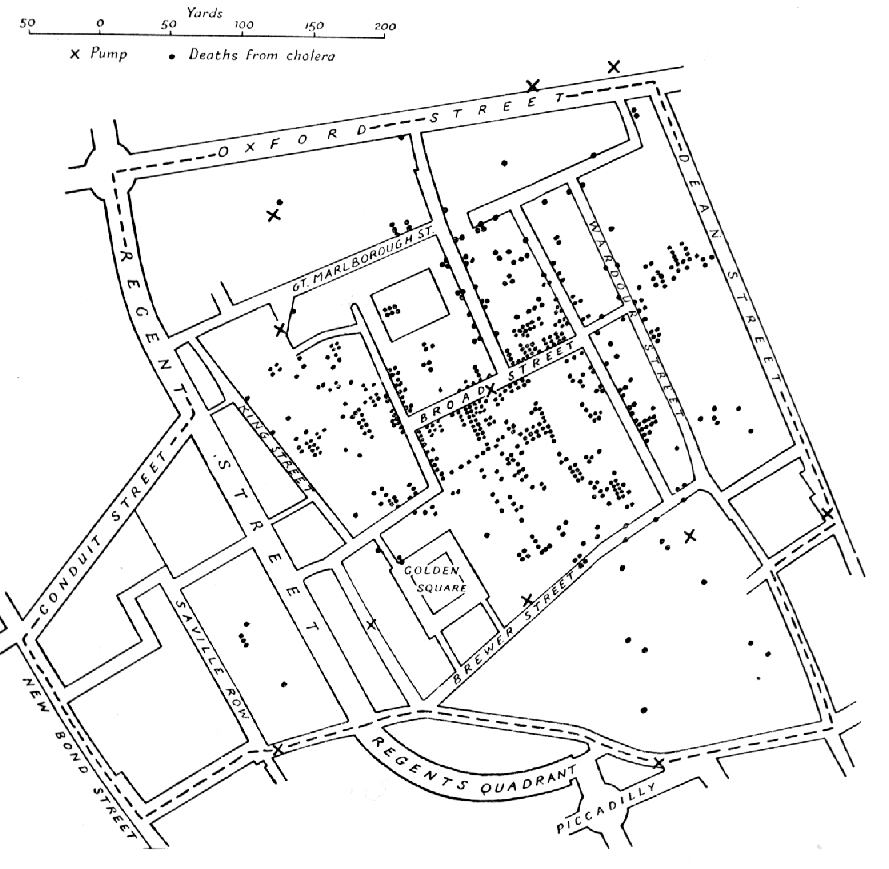
\includegraphics[scale=0.5, fbox={\fboxrule} 4mm]{images/03-antecedentes/01-cholera_map.jpg}
\caption{Mapa del Soho con los casos de fallecimiento por cólera}
\label{fig:cholera_map}
\end{figure}

Gracias a ello y referenciando en el mapa la posición de los pozos de agua, pudo comprobar como una gran cantidad de víctimas se encontraban dentro de la zona de influencia de una bomba de agua en Broad Street (ver figura \ref{fig:cholera_map_detail}), que a la postre resultó estar contaminada con heces. Recomendando la clausura de la misma consiguió acabar con la epidemia      \cite{Gunn07}. Debido a estos logros se le considera el padre de la epidemiología moderna y podemos ilustrar uno de los primeros ejemplos del uso de los \ac{SIG}.

\begin{figure}[h!btp]
\centering
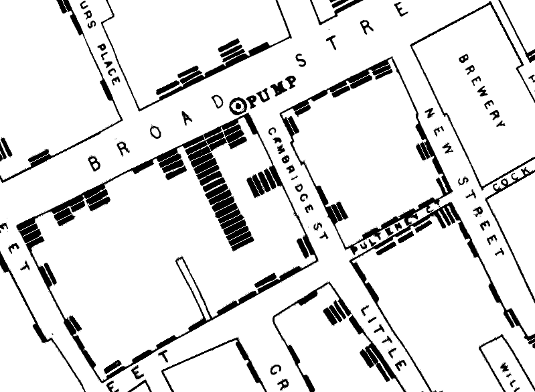
\includegraphics[scale=0.5, fbox={\fboxrule} 4mm]{images/03-antecedentes/03-cholera_map_detail.png}
\caption{Detalle del mapa del Doctor Snow}
\label{fig:cholera_map_detail}
\end{figure}

\section{Internet y la \ac{www}}

%Historia de Internet
Internet puede considerarse como una de las tecnologías que más ha cambiado el mundo y la que más rápidamente lo ha hecho. Gracias a este nuevo concepto, se puede acceder rápidamente a la mayor cantidad de información nunca antes recopilada en la historia de la humanidad.\\

La gran biblioteca de Alejandría, la mayor de las bibliotecas del mundo antiguo, contenía, según Flavio Josefo, antes de su destrucción unos 200.000 volúmenes y consideraban que todo el conocimiento de la humanidad ocuparía un total de 500.000 volúmenes  \cite{Jos94}. Autores modernos han recalculado el posible número de volúmenes, aportando una cifra de unos 50.000 rollos, que podría equivaler a unos 12.500 libros actuales \cite{Esco01}.\\

Los Archivos Secretos Vaticanos contienen un total de 1.600.000 volúmenes \cite{Bav15}, la biblioteca nacional de España 28 millones \cite{Sanz15} y la biblioteca del congreso de los \ac{EE.UU.} 160 millones de documentos \cite{Libr15}. Comparando las cifras de algunas de las mayores bibliotecas del mundo con el número de documentos existentes en Internet, podemos hacernos una idea de lo que esta tecnología a supuesto para la humanidad, no solamente en el volumen de información existente, si no en la facilidad de acceso a los mismos. En el año 2012, en Internet existían un total de 8.310 millones de documentos accesibles.

Aunque no es lícito comparar estas cifras en bruto, ya que tal la cantidad no siempre está relacionada con la calidad, como dijo el escritor Neil Gaiman \cite{Gaim10}:

\vspace{5mm}
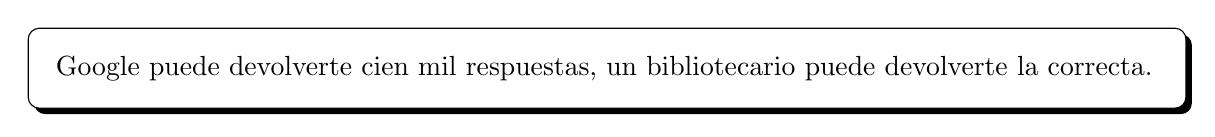
\begin{tikzpicture}
	\node[shadowBox] {
	Google puede devolverte cien mil respuestas, un bibliotecario puede devolverte la correcta.};
\end{tikzpicture}
\vspace{5mm}

En el año 1958 la compañía Bell crea el primer módem, un dispositivo capaz de transmitir datos binarios utilizando una línea telefónica (ver figura \ref{fig:bell_modem}). En el año 1962 J.C.R Licklider describe su concepto de \textit{Red galáctica}, consistente en una red interconectada globalmente que permitiera acceder a todo tipo de datos y programas desde cualquier sitio. Un año antes, en 1961, Leonard Kleinrock publicó su tesis doctoral acerca de la teoría de colas, que sería publicado como libro en el año 1964 (\cite{Klei64}) y que sirvió de fundamento a la teoría de conmutación de paquetes. Los datos se troceaban en partes, llamadas \textit{paquetes}, a los que se les asignaba un número de secuencia antes de enviarlos. De esta manera, no importaba en orden en que llegasen al receptor, puesto que podría recomponer el mensaje original.
En el año 1967 en una conferencia, se presentaba el proyecto inicial de \ac{ARPANET}. Durante las discusiones iniciales del proyecto se llegó a la conclusión de desligar la comunicación de la máquina principal, crean pequeños computadores que fuesen quienes cargasen con la responsabilidad de lidiar con las líneas telefónicas. El 29 de Octubre de 1969 se transmite el primer mensaje a través de \ac{ARPANET} y el 21 de Noviembre de ese mismo año se establece la primera conexión entre las computadoras de la universidad de Stanford y \ac{UCLA}. 

\begin{figure}[h!btp]
\centering
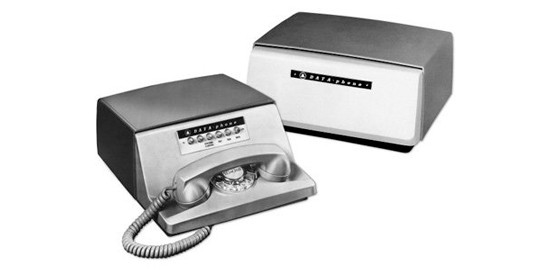
\includegraphics[scale=0.5, fbox={\fboxrule} 4mm]{images/03-antecedentes/09-modem_bell.jpg}
\caption{Módem Bell. 1958}
\label{fig:bell_modem}
\end{figure}

En el año 1972 al calor de una grande y exitosa demostración de \ac{ARPANET}, se introduce la primera gran aplicación de esta nueva tecnología, el correo electrónico. Ray Tomlinson, había desarrollado para \ac{ARPANET} unos años antes un programa llamado SNDMSG para enviar mensajes entre las distintas terminales de una computadora, por lo que adaptó este programa para permitir el envío dentro de una red más amplia.

Con el crecimiento de la red, se desarrollaron tres protocolos que actualmente siguen en uso, \ac{TCP}, \ac{IP} y \ac{DNS}. El año 1983, \ac{ARPANET} se abre definitivamente a la vida civil permitiendo el intercambio masivo de datos entre universidades y centros de investigación. Este es el motivo último por el que se celebra ese año como el nacimiento de Internet.

La \textit{web} (\ac{www}) es probablemente el punto más visible de Internet. Fue desarrollado entre 1989 y 1990 por Tim Berners-Lee y Robert Cailiau mientras trabajaban en el \ac{CERN}.

En la web, es utilizado \ac{HTTP} como protocolo de comunicación, que define la sintaxis y la semántica necesarias para el correcto funcionamiento de los distintos componentes de la comunicación web, consiguiendo una abstracción que permite unificar la forma de comunicación en la red. En las comunicaciones en red el modelo de arquitectura más extendido es el paradigma Cliente - Servidor (ver figura \ref{fig:cliente-servidor}), mediante el cual se define una máquina \textit{servidor} encargada de generar la corriente datos y una serie de máquinas conocidas como \textit{clientes}, que realizan peticiones para consumir estos datos. El funcionamiento básico de este modelo podría verse como una farmacia abierta 24 horas (servidor), que está permanentemente a la espera de que alguna persona decida entrar a comprar algún medicamento, momento en el cual busca la droga pedida y se la facilita.

\begin{figure}[h!btp]
\centering
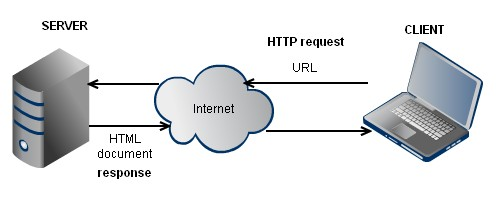
\includegraphics[scale=0.5, fbox={\fboxrule} 4mm]{images/03-antecedentes/10-client_server.png}
\caption{Modelo cliente-servidor}
\label{fig:cliente-servidor}
\end{figure}

Para que estas transacciones puedan darse, los computadores deben poder conocer como comunicarse, lo que en este caso se logra mediante las direcciones\ac{IP}, una serie de 32 bits que designan unívocamente un elemento de una red, y unos pocos pasos intermedios, y transparentes, para el usuario. El cliente, normalmente mediante un navegador web, es decir, mediante un programa creado específicamente para la navegación y visualización de páginas web, introduce el nombre de la página web con la que quiere comunicarse. Este nombre, por ejemplo, \textit{www.usipv6.com}, es enviado automáticamente a unos servidores llamados \ac{DNS}, que son capaces de buscar la dirección \ac{IP} asociada al nombre de la página tecleada y devolver su dirección \ac{IP}, que en este caso podría ser \textit{123.45.67.89} (ver figura \ref{fig:dns-server}). Es fácil ver el porque se utiliza este paso intermedio, debido a que al usuario le resultará mucho más sencillo recordar una página web que una serie de números. Una vez realizada la traducción, el computador se comunica con el servidor a través de la dirección \ac{IP} obtenida y este le responde enviándole la información solicitada.

\begin{figure}[h!btp]
\centering
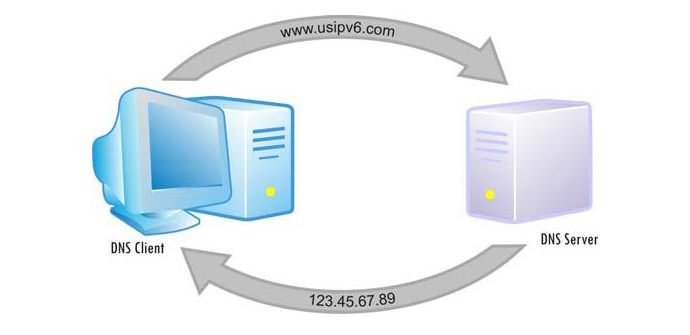
\includegraphics[scale=0.5, fbox={\fboxrule} 4mm]{images/03-antecedentes/11-dns_server.png}
\caption{Comunicación con servidor DNS}
\label{fig:dns-server}
\end{figure}

Aunque en sus orígenes,la web se desarrolló para transmitir únicamente texto, actualmente, como es fácil ver, se permite la emisión de todo tipo de contenidos multimedia, como audio, vídeo o imágenes. La tarea del cliente, consiste en recibir los datos enviados por el emisor y reinterpretarlos y mostrarlos de manera coherente para el usuario.

Todo esto nos lleva a poder diferenciar claramente dos trabajos distintos dentro de la comunicación web, el trabajo llevado a cabo por el cliente y el trabajo llevado a cabo por el servidor. Para poder desarrollar cada una de estas tareas, existen una serie de tecnologías específicas para el lado del cliente y para el lado del servidor.

\subsection{Tecnologías del lado del servidor}
Como se ha explicado en la sección anterior, el servidor es el encargado de atender las peticiones que los clientes le envían y responderlas adecuadamente. 
En los comienzos de la web los servidores eran meras estaciones de \textit{almacenaje}, que devolvía al cliente peticionario una página web estática (ver figura \ref{fig:static-server}) mientras que en la actualidad, los servidores son capaces de generar el contenido a enviar de forma dinámica (ver figura \ref{fig:dynamic-server}).

\begin{figure}[h!btp]
\centering
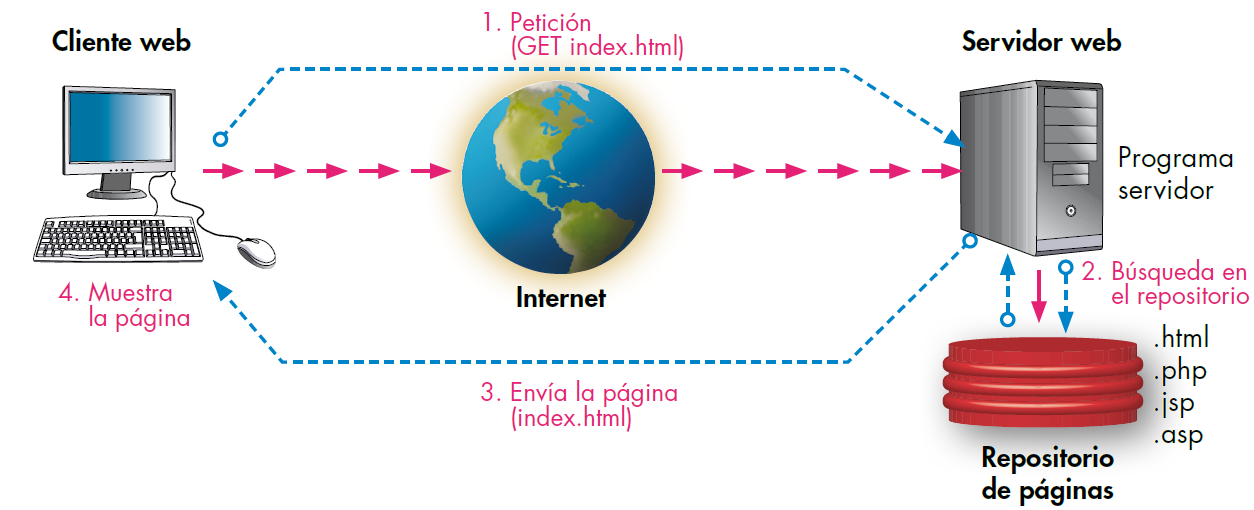
\includegraphics[scale=0.4, fbox={\fboxrule} 4mm]{images/03-antecedentes/12-html_request.png}
\caption{Petición a servidor estático}
\label{fig:static-server}
\end{figure}

\begin{figure}[h!btp]
\centering
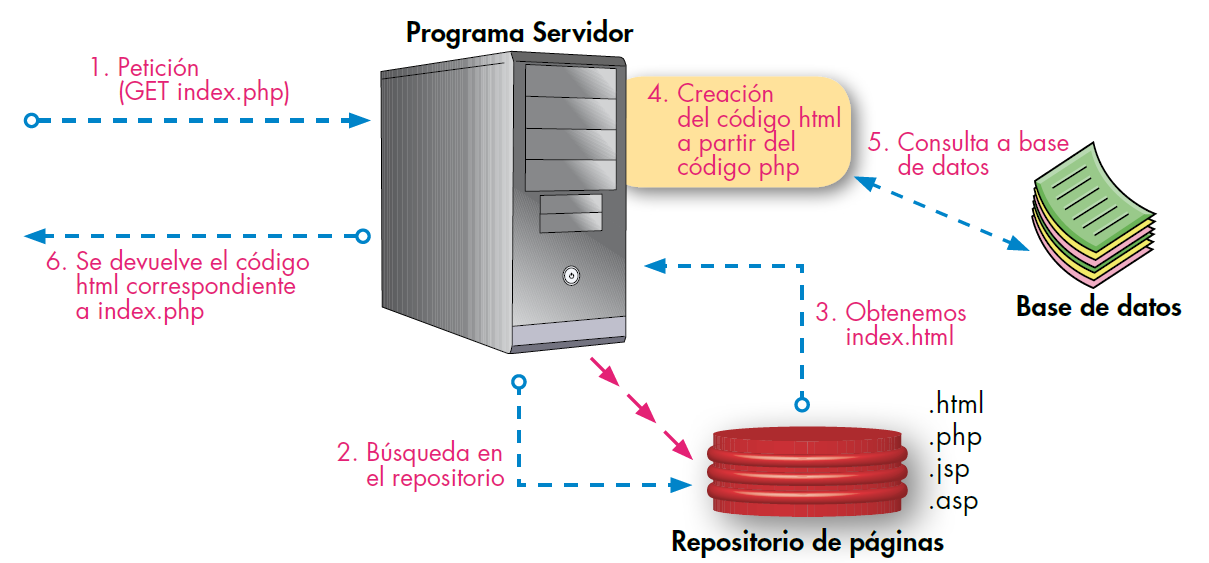
\includegraphics[scale=0.5, fbox={\fboxrule} 4mm]{images/03-antecedentes/13-html_dynamic_request.png}
\caption{Petición a servidor dinámico}
\label{fig:dynamic-server}
\end{figure}

Algunas de las tecnologías más utilizadas en el lado del cliente son Apache, PHP y MySQL.

Apache es un software que permite a un computador realizar un comportamiento de servidor, esto es, atender a las peticiones de los clientes, ofrecerles servicios y enviarles la información pedida. Esta desarrollado en C y es de código abierto \cite{Apac15}.

PHP es uno de los lenguaje de programación del lado del servidor más extendido y fue uno de los primeros en poder ser incorporado directamente en el código \ac{HTTP}. Fue creado por Rasmus Lerdorf en 1994 y actualmente se encuentra en su versión 5.6.14 \cite{Hist15}.

MySql es un sistema de gestión de bases de datos relacionales desarrollado por MySQL AB (actualmente parte de Sun Microsystems) en 1995 por Michael Widenius, David Axmark and Allan Larsson \cite{Data14}.

\begin{figure}[h!btp]
	\begin{adjustbox}{minipage=\linewidth, fbox}
		\centering
		\subfigure[MySQL]{
\includegraphics[scale=0.5]{./images/03-antecedentes/14-mysql.png}}
		\hspace{10mm}
		\subfigure[PHP]{
\includegraphics[scale=0.5]{./images/03-antecedentes/15-php.png}}
		\vspace{10mm}
		\subfigure[Apache]{
\includegraphics[scale=0.5]{./images/03-antecedentes/16-apache.png}}
	\end{adjustbox}
	\caption{Tecnologías utilizadas en servidores}
	\label{fig:mysql_php_apache}
\end{figure}

\subsection{Tecnologías del lado del cliente}
Dejando de lado la necesidad de contar con un navegador web que permita mostrar e interactuar con las páginas web mostradas, el cliente debe interpretar los datos recibidos por el servidor de manera que pueda traducirlos convirtiéndolos en el concepto de \textit{página web} que conocemos. Tres de los lenguajes más utilizados en este intercambio de datos son \ac{HTML}, \ac{CSS}, JavaScript y \ac{AJAX}.

\ac{HTML} es un lenguaje de marcado que se utiliza para la representación visual de una página web. Está considerado el lenguaje de programación más importante y está a cargo de la W3C \cite{Worl15}. Aunque permite dar formato al texto, actualmente esto suele ser responsabilidad de las hojas \ac{CSS}.

La última versión, \ac{HTML}5, publicada en octubre de 2014 \cite{Adam14} incorpora novedades como etiquetas con codecs, para manejar grandes conjuntos de datos o mejoras en los formularios.

\ac{CSS} es usado para definir el formato de una página web escrita en \ac{HTML}.

\begin{lstlisting}[
  float=ht,
  language = HTML,
  caption  = {«Hola mundo» en HTML y CSS},
  label    = code:hello]
	<!DOCTYPE html>
	<html>
	<head>
	    <title>Hola Mundo en HTML</title>
		<style>
		body {background-color:lightgrey}
		h1   {color:blue}
		p    {color:green}
		</style>
	</head>
	<body>
		<h1>Hola Mundo</h1>
		<p>Mi primera web en HTML y CSS.</p>
	</body>
	</html>
\end{lstlisting}

Javascript es un lenguaje interpretado orientado a objetos implementado normalmente como parte del navegador web.
\ac{AJAX} es utilizado para poder realizar peticiones a un servidor modificando partes concretas de una página, eliminando de esta forma la necesidad de recargar la página completa.

% Desarrollo web (frameworks)


\section{Dispositivos móviles}
Lo teléfonos móviles han cambiado nuestra manera de relacionarnos tanto con el mundo como entre las personas. No hace más de diez años era imposible pensar en poder acceder a Internet desde cualquier lugar o tener la posibilidad de enviar mensajes a través de 
las aplicaciones de mensajería instantánea. Hace veinte o treinta años nadie imaginaba que los teléfonos móviles serían un elemento imprescindible y omnipresente de nuestras vidas ya que en aquella época era símbolo de estatus y gran lujo.

Podríamos comenzar a explicar los intentos de comunicarse a través de grandes distancias con el telégrafo, primer gran antecedente del teléfono, y es que este invento fue algo revolucionario cuando se presentó. Por primera vez se podían comunicar dos puntos distantes de manera instantánea.

Los orígenes del telégrafo se remontan al S. XVIII cuando Claude Chappe desarrolló para el ejército Francés su precursor inmediato, el telégrafo óptico. Este invento consistía en un sistema de comunicación que emitía una señal visual que podía repetirse en la distancia, aunque solo tenía utilidad en las distancias a las que el ojo pudiera abarcar (ver figura \ref{fig:telegrafo_optico}) \cite{Holz94}.

\begin{figure}[h!btp]
	\begin{adjustbox}{minipage=\linewidth, fbox}
		\centering
		\subfigure[Telégrafo óptico de Claude Chappe]{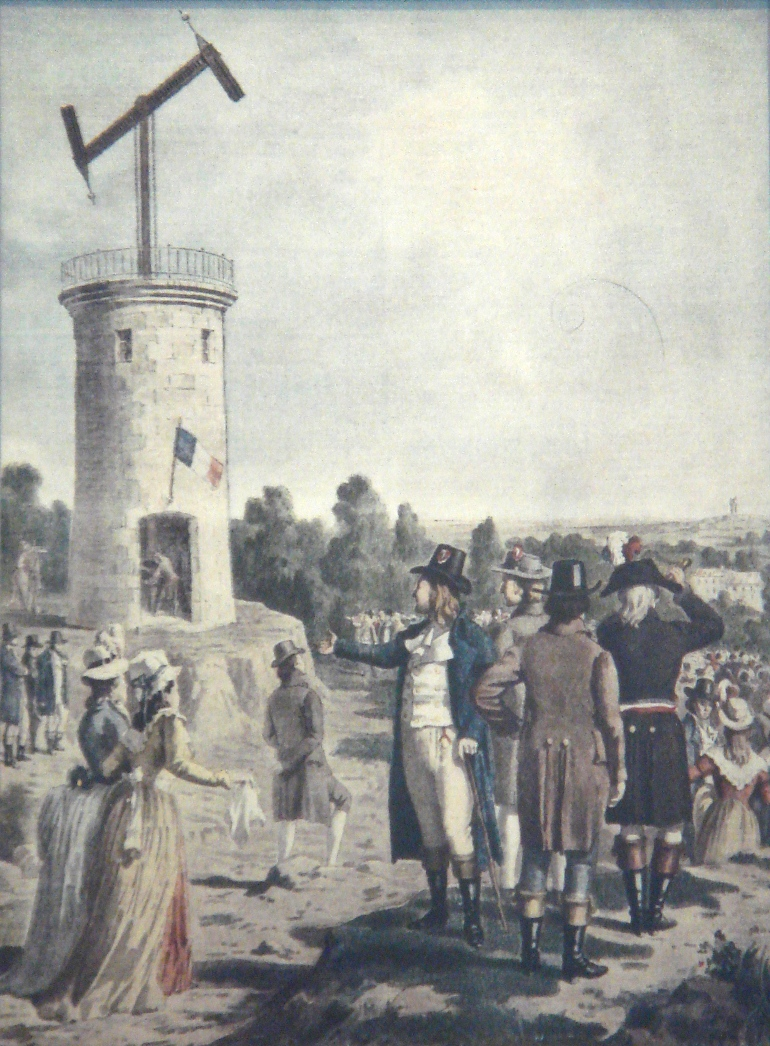
\includegraphics[height=80mm]{./images/03-antecedentes/17-telegrafo_optico.jpg}}
		\hspace{10mm}
		\subfigure[Claude Chappe]{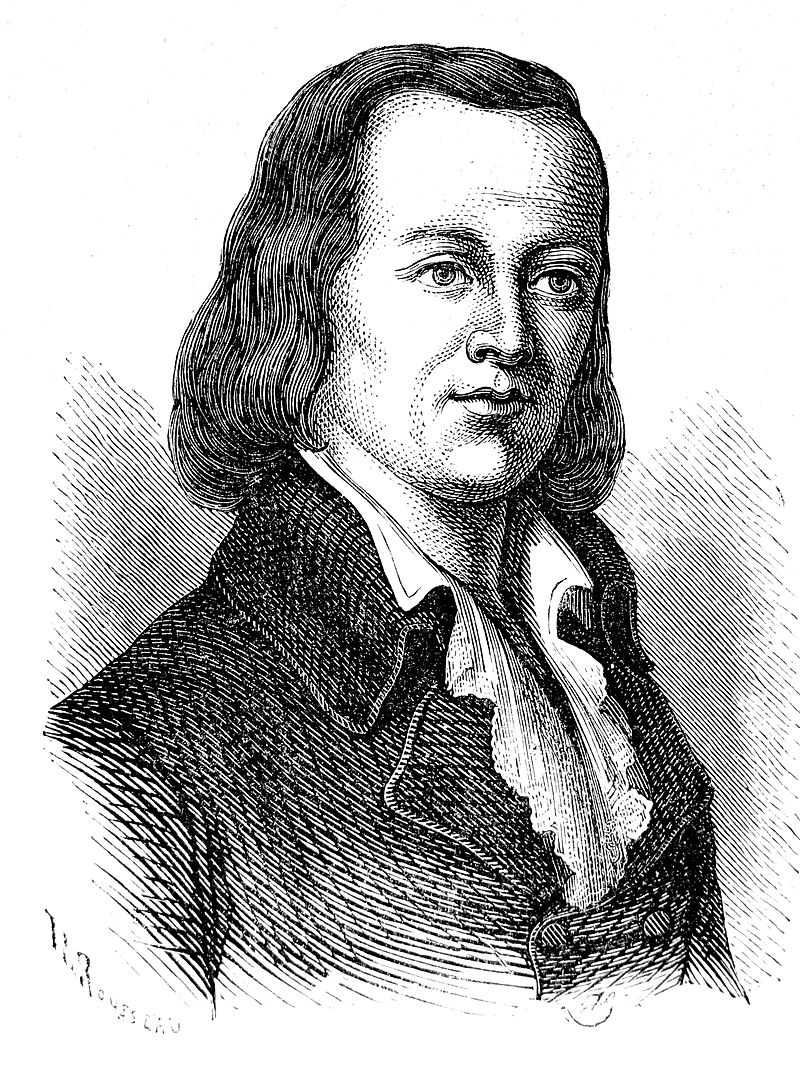
\includegraphics[height=80mm]{./images/03-antecedentes/18-claude_chappe.jpg}}
	\end{adjustbox}
\caption{Telégrafo óptico}
	\label{fig:telegrafo_optico}
\end{figure}

Con la intención de mejorar el alcance de la comunicación y aprovechando los estudios de electromagnetismo de Michael Faraday y las innovaciones de William Sturgeon y Joseph Henry sobre el electroimán, Samuel Morse (ver figura \ref{fig:telegrafo}) ideó una manera de enviar señales entre dos puntos aprovechando las corrientes eléctricas. En un primer momento, el telégrafo consistía en un péndulo que ante la existencia de corriente movía un lápiz que dibujaba de esa manera una línea sobre un papel. Mejorando el prototipo se llego a inventar el famoso código morse, que consta de los consabidos dos elementos: el punto y la raya.

\begin{figure}[h!btp]
	\begin{adjustbox}{minipage=\linewidth, fbox}
		\centering
		\subfigure[Samuel Morse]{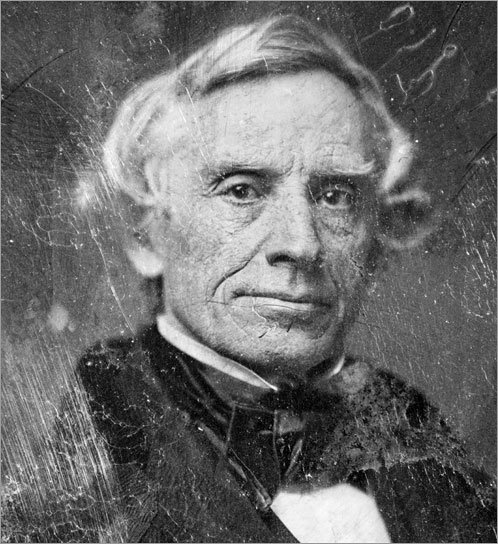
\includegraphics[height=80mm]{./images/03-antecedentes/20-samuel_morse.jpg}}
		\hspace{10mm}
		\subfigure[Código morse]{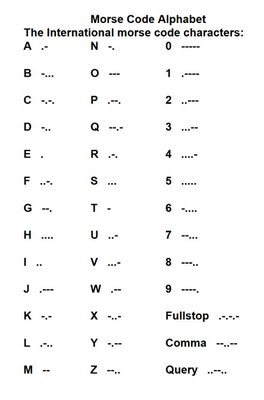
\includegraphics[height=80mm]{./images/03-antecedentes/21-codigo_morse.jpg}}
	\end{adjustbox}
\caption{Telégrafo}
	\label{fig:telegrafo}
\end{figure}

En 1837 Samuel Morse hizo la primera demostración pública del telégrafo en un áula de la universidad de Nueva York. La gran aportación de Morse.

El 24 de mayo de 1844, se terminó la línea que unía Baltimore y Washington, enviando un mensaje desde la Cámara de Corte Suprema de en el Capitolio de \ac{EE.UU.} en Washington hasta el ferrocarril B \& O en Baltimore con la frase \textit{What hath God wrought?} perteneciente al libro de los Números (ver figura \ref{fig:telegrama}).

\begin{figure}[h!btp]
\centering
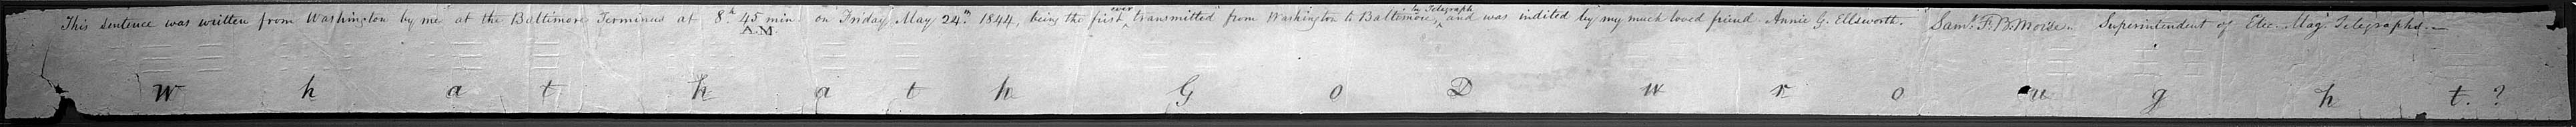
\includegraphics[width=100mm, fbox={\fboxrule} 4mm]{images/03-antecedentes/19-primer_telegrama.jpg}
\caption{Primer telegrama}
\label{fig:telegrama}
\end{figure}

El siguiente gran paso en las comunicaciones viene de la mano de un dispositivo capaz de retransmitir, a través de cables, las señales acústicas derivadas de la voz humana. El teléfono.

Históricamente, la invención del teléfono se atribuyó a Alexander Graham Bell \cite{Cab79}, aunque el 11 de junio de 2002 fue reconocido el italiano Antonio Meucci (ver figura \ref{fig:teléfono}) como el verdader inventor de este aparato por el Congreso de los Estados Unidos \cite{Uni03}.

\begin{figure}[h!btp]
	\begin{adjustbox}{minipage=\linewidth, fbox}
		\centering
		\subfigure[Antonio Meucci]{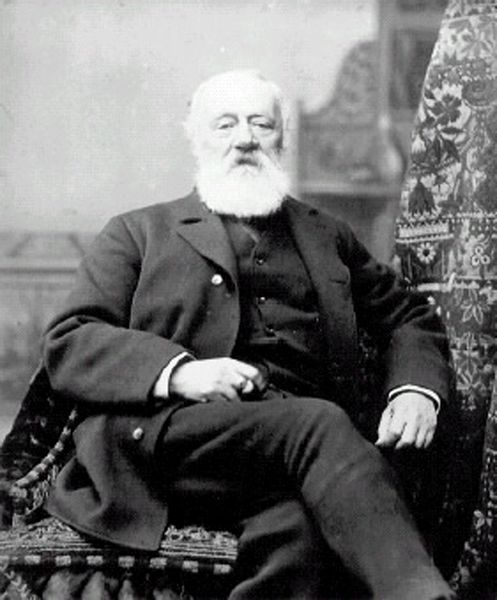
\includegraphics[height=80mm]{./images/03-antecedentes/22-antonio_meucci.jpg}}
		\hspace{10mm}
		\subfigure[Alexander Graham Bell]{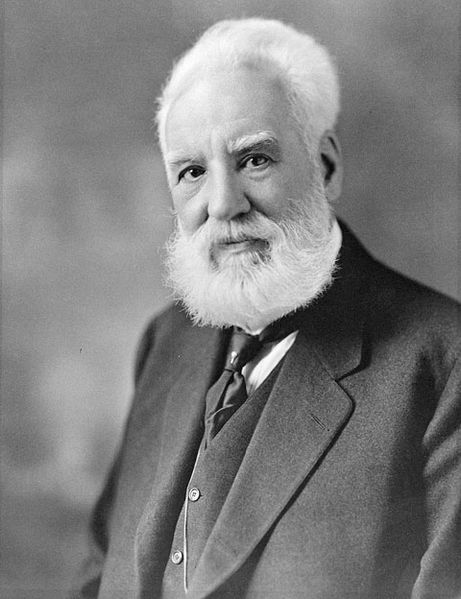
\includegraphics[height=80mm]{./images/03-antecedentes/23-alexander_graham_bell.jpg}}
	\end{adjustbox}
\caption{Inventores del teléfono}
	\label{fig:teléfono}
\end{figure}

Antonio Meucci, nacido en Florencia, emigró junto a su esposa Ester Mochi primero a Cuba en octubre de 1835 y después a Staten Island, Nueva York \ac{EE.UU.} en 1850.

Ya que vivían en una casadevarios pisos y debido al reumatismo de su esposa, Meucci construyó el primer teléfono alrededor de 1857, que consistía en un aparato que permitía comunicar su despacho con el  dormitorio donde se encontraba su esposa debido a la enfermedad \cite{Meuc10}. El 28 de diciembre de 1871 presentó la documentación previa a la patente, pero solo consiguió el dinero para renovarla en 1872 y 1873. Meucci ofreció una demostración de su \textit{teletrófono} a la \textit{Western Union Telegraph Company} pero viendo la falta de interés de la empresa en su desarrollo, pidió que la devolución de los materiales presentados, a lo que contestaron diciendo que habían sido perdidos.

Aunque este hecho no está probado, parece ser que estos materiales cayeron en manos de Alexander Graham Bell, que en aquella época trabajaba en los laboratorios de la compañía utilizándolos más tarde para desarrollar su propio teléfono. En 1876, Bell presentó, unas horas antes que su compatriota Elisha Gray, la patente de su teléfono. 

Ante las reclamaciones de Meucci de la autoría del invento, y gracias a la intervención de un amigo, se pudo saber que las patentes relacionadas con el \textit{telégrafo parlante}, se habían extraviado. En investigaciones posteriores se descubrieron pagos a funcionarios por parte de Bell para hacer desaparecer estos documentos. Debido a las pruebas de prevaricación, en 1886 el Secreatrio de Estado llegó a confirmar que existían suficientes pruebas para otorgar la autoría del invento a Antonio Meucci. La demanda cesó como consecuencia de la muerte del demandante en octubre de 1889, después de que los abogados de Bell consiguieran dilatar el proceso mediante recursos judiciales. Como curiosidad, Thomas Alva Edison enviaría una carta al juez posicionándose a favor de Meucci en sus reivindicaciones \cite{Carb07}.

\begin{figure}[h!btp]
	\begin{adjustbox}{minipage=\linewidth, fbox}
		\centering
		\subfigure[Teléfono de Meucci]{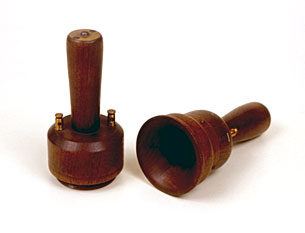
\includegraphics[scale=0.5]{./images/03-antecedentes/24-telefono_meucci.jpg}}
		\hspace{10mm}
		\subfigure[Teléfono de Bell]{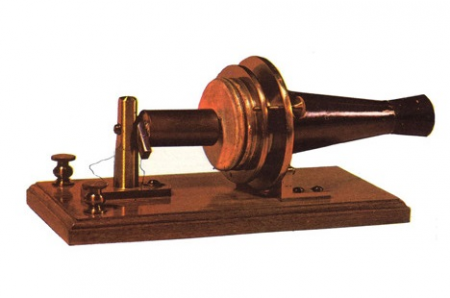
\includegraphics[scale=0.5]{./images/03-antecedentes/25-telefono_bell.png}}
	\end{adjustbox}
\caption{Primeros teléfonos}
	\label{fig:primeros-teléfonos}
\end{figure}


El 9 de octubre de 1876 se realizó una demostración en la Bell y su ayudante Thomas Watson mantuvieron una conversación telefónica entre Cambridge y Boston. La primera frase pronunciada durante este evento fue \textit{"Mr. Watson, come here. I want to see you."} \cite{Even01}.

Dejando de lado los primeros intentos de readiotelefonía, el primer teléfono móvil fue desarrollado por Motorola en 1983. El modelo \ac{DynaTAC} 8000x que tenía una autonomía de 1 hora y permitía treinta minutos de conversación. El precio de venta al público se estableción en casi 4.000 dólares.

Aunque la comercialización se llevo a cabo en la  mencionada fecha, la primera llamada se realizó diez años antes, en abril de 1973 por Martin Cooper, director de Motorola al teléfono fijo de Joel Engel, investigador de los laboratorios Bell, su principal competidora. En una entrevista para la BBC, Cooper comentaba cómo se desarrolló esa primera conversación: "Joel it's Martin and i'm calling you from a cell phone but a real cell phone" \cite{BBC13}\footnote{Cómo curiosidad se incluye el enlace al vídeo promocional del DynaTAC 8000X \url{https://www.youtube.com/watch?v=0WUF3yjgGf4}}.

\begin{figure}[h!btp]
	\begin{adjustbox}{minipage=\linewidth, fbox}
		\centering
		\subfigure[Motorola DynaTAC 8000X]{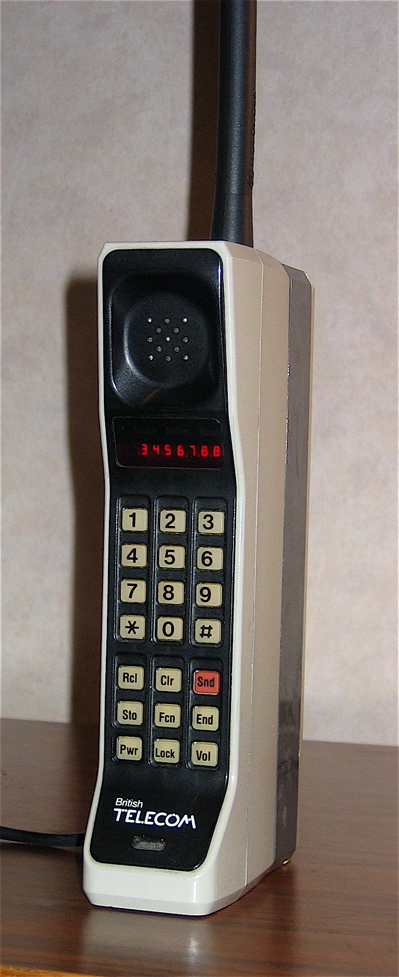
\includegraphics[height=45mm]{./images/03-antecedentes/27-motorola-dynatac_8000x.jpg}}
		\hspace{10mm}
		\subfigure[Martin Cooper]{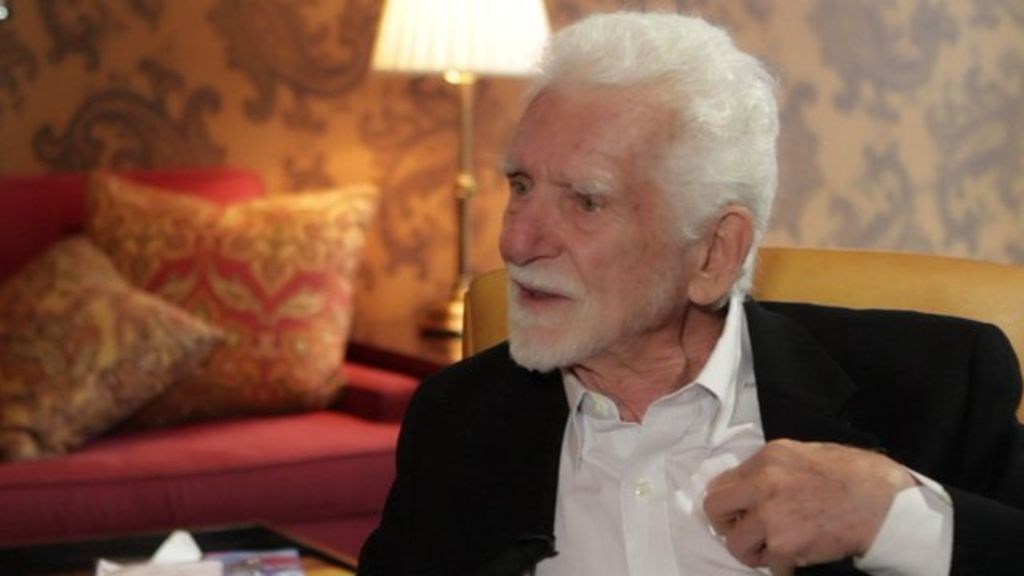
\includegraphics[width=80mm]{./images/03-antecedentes/28-martin_cooper.jpg}}
	\end{adjustbox}
\caption{Primeros teléfonos}
	\label{fig:primeros-teléfonos}
\end{figure}

La gran novedad de estos primeros modelos sobre los aparatos de radiotelefonía es que podían ser trasladados y manejados por una sola persona.

La primera generación de teléfonos móviles se desarrolló hasta finales de los años 80. Estos primeros modelos únicamente permitían el intercambio de voz.

La segunda generación llego en los años 90, poniendo el acento en la digitalización de las comunicaciones, ya que ofrecían un aumento sustancial de la calidad de voz y se simplificaba la fabricación reduciendo los costes. En este momento se integró un de los servicios más populares de los teléfonos móviles hasta la aparición de la mensajería instantánea, los \ac{SMS}.

\begin{figure}[h!btp]
\centering
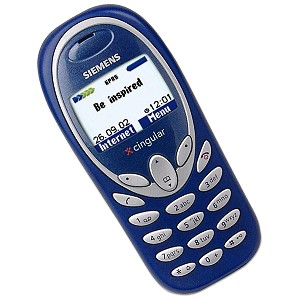
\includegraphics[height=40mm, fbox={\fboxrule} 4mm]{images/03-antecedentes/29-siemens_a56.jpg}
\caption{Teléfono de segunda generación. Siemens A56}
\label{fig:siemens-a56}
\end{figure}

El siguiente gran salto vino de la mano de Apple y su iPhone, sacado al mercado en el año 2007. Con un diseño estudiado y una pantalla multitáctil, aprovechando la buena imagen de marca conseguida a través del iPod, Apple sacó un teléfono que revolucionó la manera en la que hasta entonces se entendían los teléfonos. Siendo una mezcla de teléfono, ordenador, reproductor de música, agenda personal y reproductor multimedia, no tardó en convertirse en un producto casi imprescindible para el consumidor y por tanto algo a imitar por las compañías rivales. Había nacido la era de los smartphones.

\begin{figure}[h!btp]
\centering
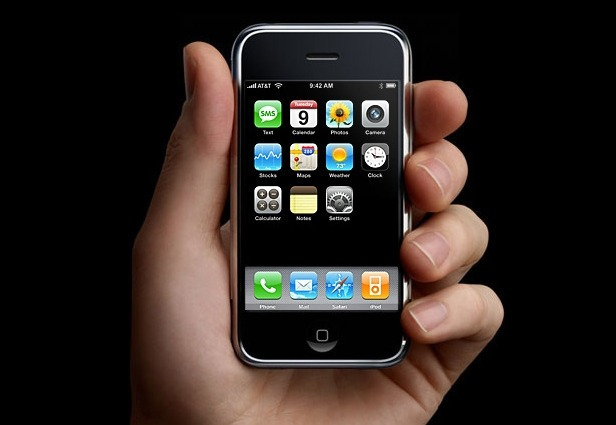
\includegraphics[width=60mm, fbox={\fboxrule} 4mm]{images/03-antecedentes/30-iphone.jpg}
\caption{iPhone de Apple}
\label{fig:iphone}
\end{figure}

\section{Aplicaciones similares}
En este apartado presentaremos aplicaciones similares a la que se pretende desarrollar. El parecido viene dado bien por el uso de la localización, bien por la compartición de la ubicación o bien por ser aplicaciones con la misma finalidad que la desarrollada en el presente \ac{TFG}.

\subsection{Foursquare}
Sin duda alguna, Foursquare (\url{https://es.foursquare.com/}) es la aplicación más conocida de las presentadas. Fue creada en 2009 por Dennis Crowley y Naveen Selvadurai. Básicamente consistía en una red social que permitía indicar el punto geográfico en el que el usuario se encuentra en ese momento\cite{Rubi13} y opinar acerca del lugar, establecimiento o comercio y mostrar los puntos de interés cercanos a su posición \cite{Cano14}. 

Esta aplicación está disponible para \href{https://play.google.com/store/apps/details?id=com.joelapenna.foursquared}{Android}, \href{https://itunes.apple.com/us/app/id306934924?mt=8}{iOS} y \href{https://www.microsoft.com/es-es/store/apps/foursquare/9wzdncrfhw3v}{Windows Mobile}.

\begin{figure}[h!btp]
	\begin{adjustbox}{minipage=\linewidth, fbox}
		\centering
		\subfigure[Aplicación Foursquare en funcionamiento]{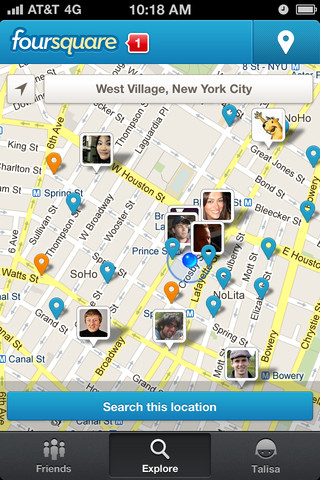
\includegraphics[scale=0.6]{./images/03-antecedentes/50-foursquare_app.jpg}}
		\hspace{10mm}
		\subfigure[Logo de Foursquare]{
\includegraphics[width=40mm, fbox={\fboxrule} 4mm]{images/03-antecedentes/38-foursquare.png}}
	\end{adjustbox}
\caption{Foursquare}
	\label{fig:foursquare}
\end{figure}

\subsection{Swarm}
En el año 2014 Foursquare lanza Swarm (\url{https://es.swarmapp.com/}), que es una escisión dedicada más a compartir la posición y permitir concertar lugares de encuentro y saber que contactos tenemos cerca dejando de lado la parte lúdica y la compartición de experiencias, que se traslada definitivamente a Foursquare \cite{Buzz14}.

Esta aplicación está disponible para \href{https://play.google.com/store/apps/details?id=com.foursquare.robin}{Android}, \href{https://itunes.apple.com/US/app/id870161082?mt=8}{iOS} y \href{https://www.microsoft.com/es-es/store/apps/swarm/9wzdncrdrsq1}{Windows Mobile}.

\begin{figure}[h!btp]
\centering

\includegraphics[scale=0.25, fbox={\fboxrule} 4mm]{images/03-antecedentes/39-swarm.png}
\caption{Logo de Swarm}
\label{fig:swarm}
\end{figure}

\subsection{Glympse}
Glympse (\url{https://www.glympse.com/}) es una aplicación que permite compartir en tiempo real la ubicación del usuario con los contactos que desee. Es una forma rápida de indicar y compartir la posición en la que te encuentras, viniendo a responder a la pregunta,"¿Dónde te encuentras en este momento?", sin necesidad de abrir el móvil. Los destinatarios de los "Glympses" no necesitan tener instalada la aplicación para acceder a nuestros recorridos \cite{Unk15}.

Esta aplicación está disponible para \href{https://play.google.com/store/apps/details?id=com.glympse.android.glympse}{Android}, \href{https://itunes.apple.com/app/glympse-share-gps-location/id330316698?mt=8}{iOS} y \href{https://www.microsoft.com/es-es/store/apps/glympse/9wzdncrdf9sj}{Windows Mobile}.

\begin{figure}[h!btp]
	\begin{adjustbox}{minipage=\linewidth, fbox}
		\centering
		\subfigure[Aplicación Glympse en funcionamiento]{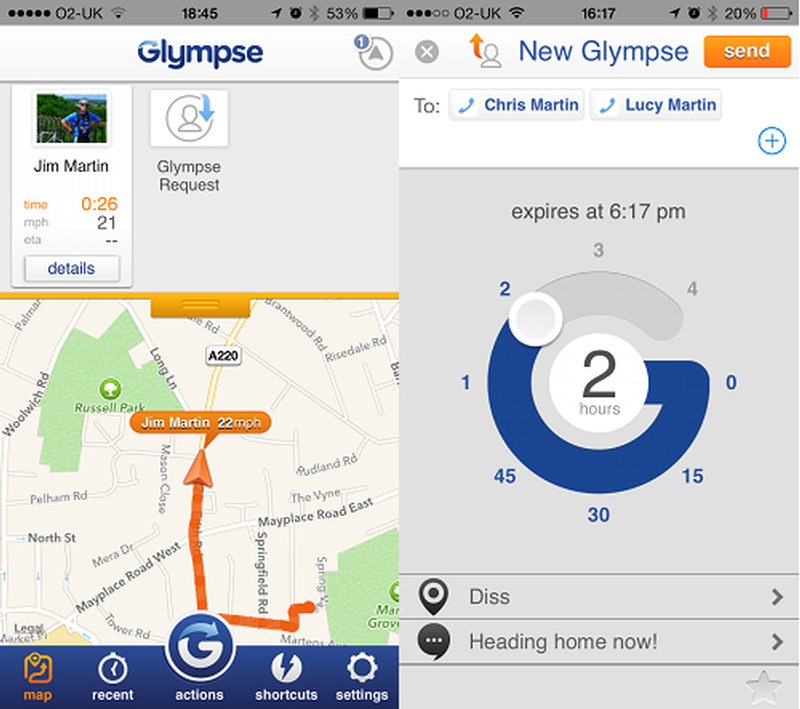
\includegraphics[scale=0.3]{./images/03-antecedentes/40-glympse_app.png}}
		\hspace{10mm}
		\subfigure[Logo Glympse]{\includegraphics[width=40mm]{./images/03-antecedentes/41-glympse_logo.png}}
	\end{adjustbox}
\caption{Glympse}
	\label{fig:glympse}
\end{figure}

\subsection{Strava}
Strava (\url{https://www.strava.com/}) es una aplicación que permite hacer un seguimiento al usuario mientras realiza actividades deportivas. Permite el seguimiento entre usuarios y genera estadísticas de rendimiento que pueden ser comparadas. Puede utilizarse a través de la página web, sin necesidad de descargarse las distintas aplicaciones \cite{Moya12}.

Esta aplicación está disponible para \href{https://play.google.com/store/apps/details?id=com.strava}{Android} y \href{https://itunes.apple.com/app/strava-cycling/id426826309?mt=8}{iOS}.

\begin{figure}[h!btp]
	\begin{adjustbox}{minipage=\linewidth, fbox}
		\centering
		\subfigure[Aplicación Strava en funcionamiento]{\includegraphics[width=120mm]{./images/03-antecedentes/42-strava_app.jpg}}
		\hspace{10mm}
		\subfigure[Logo Strava]{\includegraphics[width=40mm]{./images/03-antecedentes/43-strava_logo.png}}
	\end{adjustbox}
\caption{Strava}
	\label{fig:strava}
\end{figure}

\subsection{Waze}
Waze (\url{https://www.waze.com/es/}) es una aplicación que permite compartir en tiempo real información sobre el estado del tráfico, de manera que recibas y envíes el estado de las carreteras a todos aquellos usuarios de la comunidad conectados en ese momento. Permite adecuar las rutas de tráfico en función de los atascos detectados, informa de los precios de las gasolineras y permite avisar al resto de conductores de la posición de patrullas de tráfico o radares, último aspecto este que le ha dado gran controversia \cite{Cast13}. También permite interactuar automáticamente con Foursquare, marcando la posición de llegada justo al terminar el viaje, y con otras redes sociales como Facebook o Twitter \cite{Pen11}. A mediados de 2013 fue adquirida por Google por un total de 966 millones de dólares \cite{ABC13}.

Esta aplicación está disponible para \href{https://play.google.com/store/apps/details?id=com.waze}{Android}, \href{https://itunes.apple.com/us/app/waze-social-gps-traffic/id323229106?mt=8}{iOS} y \href{https://www.microsoft.com/es-es/store/apps/waze/9wzdncrfj2m3}{Windows Mobile}.

\begin{figure}[h!btp]
	\begin{adjustbox}{minipage=\linewidth, fbox}
		\centering
		\subfigure[Aplicación Waze en funcionamiento]{\includegraphics[scale=0.3]{./images/03-antecedentes/45-waze_app.jpg}}
		\hspace{10mm}
		\subfigure[Logo Waze]{\includegraphics[width=40mm]{./images/03-antecedentes/44-waze_logo.png}}
	\end{adjustbox}
\caption{Waze}
	\label{fig:waze}
\end{figure}

\subsection{Ingress}

Como curiosidad del uso de los gps y la comunicación social, alejándonos de lo habitual, se encuentra Ingress (\url{https://www.ingress.com/}), un juego de realidad aumentada a través de gps que permite "conquistar" zonas de interés mientras estés cerca de ellas. Estas zonas normalmente coinciden con puntos emblemáticos y conocidos de las ciudades. La interacción social se consigue debido a que existen dos bandos enfrentados por conseguir los recursos de las zonas. Este juego está desarrollado por Niantic y distribuido por Google \cite{Pen13}.

Desde diciembre de 2013 está disponible para \href{https://play.google.com/store/apps/details?id=com.nianticproject.ingress}{Android} mientras que el lanzamiento para \href{https://itunes.apple.com/us/app/ingress/id576505181?mt=8}{iOS} fue en julio de 2014.

\begin{figure}[h!btp]
	\begin{adjustbox}{minipage=\linewidth, fbox}
		\centering
		\subfigure[Aplicación Ingress en funcionamiento]{\includegraphics[height=80mm]{./images/03-antecedentes/46-ingress_app.png}}
		\hspace{10mm}
		\subfigure[Logo Ingress]{\includegraphics[width=40mm]{./images/03-antecedentes/47-ingress_logo.png}}
	\end{adjustbox}
\caption{Ingress}
	\label{fig:ingress}
\end{figure}

\subsection{Life360 Family Locator}
El concepto que subyace detrás de esta aplicación (\url{https://www.life360.com/family-locator/} es extremadamente sencillo, tener localizados en un mapa a todos los miembros de una familia mediante el gps del móvil \cite{Unk13}.

Esta aplicación está disponible para \href{https://play.google.com/store/apps/details?id=com.life360.android.safetymapd}{Android}, \href{https://itunes.apple.com/us/app/life360-locator/id384830320?mt=8}{iOS} y \href{https://www.microsoft.com/es-es/store/apps/life360-family-locator/9wzdncrfj0gw}{Windows Mobile}.

\begin{figure}[h!btp]
	\begin{adjustbox}{minipage=\linewidth, fbox}
		\centering
		\subfigure[Aplicación Life360 Family Locator en funcionamiento]{\includegraphics[height=80mm]{./images/03-antecedentes/48-life360_app.jpg}}
		\hspace{10mm}
		\subfigure[Logo Life360 Family Locator]{\includegraphics[width=40mm]{./images/03-antecedentes/49-life360_logo.png}}
	\end{adjustbox}
\caption{Life360 Family Locator}
	\label{fig:life360}
\end{figure}

\subsection{¿Dónde está mi coche?}
Esta aplicación guarda la ubicación marcada por el gps en cuanto pierda la conexión bluetooth con del coche \cite{Unk14}.

Está disponible para \href{https://play.google.com/store/apps/details?id=com.whereismycar&hl=es}{Android} e \href{https://itunes.apple.com/es/app/donde-esta-mi-coche/id504186557?mt=8}{iOs}.

\subsection{Find my car}
Aplicación que almacena la posición indicada por el gps cuando el usuario lo solicita. Permite acciones secundarias como cronometrar el tiempo que pasas desde que has aparcado, mostrar el camino de vuelta o sacar fotos del lugar de aparcamiento \cite{Unk14}.

Está disponible para \href{https://play.google.com/store/apps/details?id=com.elibera.android.findmycar&hl=es}{Android} e \href{https://itunes.apple.com/us/app/find-my-car/id349510601?mt=8}{iOs}.

% Local Variables:
%  coding: utf-8
%  mode: latex
%  mode: flyspell
%  ispell-local-dictionary: "castellano8"
% End:

\chapter{Método de Trabajo}
\label{chap:metodo}

\drop{E}{n} este capítulo se detalla la metodología utilizada para el desarrollo del presente \ac{TFG} así como las tecnologías utilizadas para llevar a término el proyecto.

Para la gestión dek proyecto se usará Scrum y como soporte del \ac{TFG} se utilizará Kanban haciendo uso del desarrollo evolutivo.

Scrum proporciona elmarco de trabajo Kanban proporciona un método productivo bien delineado en fases que garantiza que el cambio a la siguiente fase no se producirá hasta haberse completado correctamente la fase actual.

El desarrollo del producto software se realizará mediante prototipado evolutivo, ya que es una solución que permite asegurarse del correcto funcionamiento de los componentes antes de permitir el siguiente paso, también conseguiremos de esta manera ir perfilando el producto final mediante un acercamiento por fases terminadas.

Por tanto, el prototipado nos marcará la meta de cada fase, Kanban nos indicará los objetivos individuales necesarios para alcanzar el final de cada una de las fases y Scrum nos proporcionará un marco de trabajo adecuado para la consecución de los objetivos.


\section{Dispositivos empleados}
\label{section:dispositivos-empleados}
Para el desarrollo del \ac{TFG} se utilizarán los siguientes dispositivos:

	\subsection{Ordenador portátil}
	
	Para el desarrollo del TFG se ha utilizado un ordenador portátil con las características que se detallan en la tabla \ref{tab:portatil}.
	
	\begin{table}[H]
	  \centering 
	  \rowcolors{1}{gray!25}{white}
	  \begin{tabular}{p{0.4\linewidth}p{0.3\linewidth}}
	    \toprule
	    Fabricante 							& Acer 											\\
	    Modelo								& Aspire V 15 Nitro								\\
		Fabricante Procesador 				& Intel 										\\
		Modelo Procesador 					& i7-5500U 										\\
		Velocidad y Núcleos del Procesador & 2.4 GHz; 2 núcleos 							\\
		Memoria RAM 						& 16 \ac{GB} \ac{DDR}3L \ac{SDRAM} 			\\
		Disco Duro Principal y Secundario 	& 250 \ac{GB} \ac{SDD} y 1 \ac{TB} \ac{HDD}	\\
		Sistema Operativo					& Elementary \ac{OS} 							\\
	    \hline
	  \end{tabular}
	  \caption{Ordenador utilizado para el desarrollo \ac{TFG}}
	  \label{tab:portatil}
	\end{table}
	
	\subsection{Teléfono móvil}
	
	Para las pruebas del desarrollo en dispositivos móviles se ha utilizado un teléfono móvil con las características que se detallan en la tabla \ref{tab:movil}.
	
	\begin{table}[H]
	  \centering 
	  \rowcolors{1}{gray!25}{white}
	  \begin{tabular}{p{0.4\linewidth}p{0.3\linewidth}}
	    \toprule
	    Fabricante 				& LG 				\\
	    Modelo 					& D820 (Nexus 5) 	\\
		Fabricante Procesador 	& Qualcomm 			\\
		Modelo Procesador 		& Snapdragon 800 	\\
		Velocidad Procesador 	& 2.26 GHz 			\\
		Memoria RAM 			& 2 \ac{GB} 		\\
		Sistema Operativo 		& Android 6.0 		\\
		Tamaño Pantalla			& 4.95 pulgadas 	\\
	    \hline
	  \end{tabular}
	  \caption{Dispositivo móvil utilizado para el desarrollo \ac{TFG}}
	  \label{tab:movil}
	\end{table}

\section{Desarrollo evolutivo}
\label{section:desarrollo}
También conocido como prototipado evolutivo, este tipo de desarrollo se basa en exponer una implementación inicial al usuario permitiendo, a través de sus comentarios, refinar el sistema mediante versiones hasta alcanzar el producto final.
Este tipo de enfoque es más efectivo que un desarrollo en cascada debido a que satisface las necesidades inmediatas del cliente y debido a que utiliza un enfoque evolutivo, la especificación del producto se desarrolla de forma creciente en tanto en cuanto el cliente comienza a mejorar su comprensión y acercamiento al problema que pretende solucionar.
Debido a su propia naturaleza, el buen funcionamiento de este tipo de desarrollo, requiere de una gran vinculación por parte del cliente, que en este caso estará representado por el director del proyecto, ya que el elemento más importante en este prototipado, es la retroalimentación proveniente de numerosas entrevistas que ayuden a marcar el rumbo del desarrollo \cite{Somm06}.

\begin{figure}[H]
\centering
\includegraphics[width=120mm, fbox={\fboxrule} 4mm]{images/04-metodo/01-protipado_evolutivo.jpg}
\caption{Prototipado Evolutivo}
\label{fig:prototipado_evolutivo}
\end{figure}

\section{Scrum}
Scrum es un marco de trabajo de procesos usado desde principios de los años 90. Al ser un marco de trabajo no puede utilizarse para como una técnica o un proceso para construir algo, si no que nos propone una serie de métodos para alcanzar el objetivo final.
El marco de trabajo consiste en los \textit{Equipos Scrum}, \textit{roles}, \textit{eventos}, \textit{artefactos} y \textit{reglas}.
Las reglas son las que relacionan los eventos, roles y artefactos, dotando de orden las interacciones entre estos elementos.
Scrum se basa en el conocimiento empírico, esto es,el conocimiento se basa en la experiencia y la toma de decisiones debe estar basada en este precepto \cite{Sch13}.
Los tres pilares básicos de este marco de trabajo son la \textbf{transparencia}, \textbf{inspección} y \textbf{adaptación}.
La transparencia consiste en permitir que los aspectos significativos sean visibles para los responsables del resultado, que deben tener un lenguaje asociado común y la compartición de los términos importantes, por ejemplo, todos los miembros deben tener el mismo concepto de \textit{producto terminado}.
La inspección consiste en que los artefactos deben ser frecuentemente revisados en su progreso hacia el objetivo marcado, para detectar posibles problemas, errores o desviaciones. Estas inspecciones no deben entorpecer el trabajo habitual.
Cuando se detectan desviaciones durante el proceso de inspección, entra en liza la adaptación, que consiste en reconducir la situación hacia los cauces normales y aceptables de calidad marcados previamente.

\subsection{Equipo scrum}
El \textit{equipo scrum} está formado por un \textit{Product Owner}, \textit{Development Team} y un \textit{Scrum Master}. Los equipos son autoorganizados y multifuncionales, lo que significa que el propio equipo elige la forma de llevar a cabo el trabajo sin ser dirigidos por personas externas y mantienen todas las competencias necesarias para finalizar el trabajo.
Scrum obliga a realizar entregas de forma iterativa e incremental, de manera que la retroalimentación es constante y permite disponer en todo momento de una versión funcional y potencialmente útil del producto.

El \textit{Product Owner} es el encargado de gestionar el \textit{Product Backlog}, consistente en una lista ordenada de los elementos necesarios para la realización del producto terminado. El \textit{Product Owner} es una única persona física, que en el caso particular del presente trabajo corresponde al director del proyecto.

El \textit{Development Team} es el equipo de profesionales encargado de desarrollar el trabajo que desemboque en el producto \textit{terminado}. En el caso particular del presente trabajo, este rol corresponde al autor del mismo.

El \textit{Scrum Master} es el responsable de que el \textit{Equipo Scrum} entiende y aplica la teoría, prácticas y reglas de Scrum.

\subsection{Eventos de scrum. El sprint}
Los eventos en Scrum están predefinidos para evitar las reuniones no definidas por el marco. El centro de Scrum son los sprints, un bloque de tiempo improrrogable e inacortable que finaliza con un incremento de producto \textit{Terminado}. Este evento mantiene varios subeventos que lo dotan de alcance: \textit{Sprint Planning Meeting}, \textit{Daily Scrums}, trabajo de desarrollo, \textit{Sprint Review} y \textit{Sprint Retrospective}.

Las reglas aplicables al Sprint no permiten realizar cambios que afecten al objetivo del mismo, ni disminuir los objetivos de calidad, aunque en cambio si permite aclarar y renegociar el alcance del proyecto entre el \textit{Product Owner} y el \textit{Development Team} a medida que van conociéndose con más detalle los objetivos finales.

Los Sprint están limitados temporalmente a un máximo de un mes de trabajo, no pudiéndose alargar este plazo bajo ningún concepto. Pueden ser cancelados únicamente por el \textit{Product Owner} en caso de quedar el objetivo planificado obsoleto.

El \textit{Sprint Planning Meeting} crea un plan de trabajo para el sprint que va a desarrollarse. Al igual que con el sprint, también existe una regla de duración máxima, que lo fija en un total de ocho horas para un sprint de un mes.
En esta reunión se deben responder a las siguientes cuestiones:
\begin{itemize}[label={$\bullet$},labelindent=\parindent,leftmargin=2cm]
	\item ¿Qué se entregará al finalizar el incremento del sprint?
	\item ¿Qué acciones son necesarias para llevarlo a cabo?
\end{itemize}
En este momento se deciden que elementos del \textit{Product Backlog} van a ser tomados para su desarrollo y se traza un plan para conseguirlo.

Durante el \textit{Daily Scrums}, una reunión realizada a diario con un bloque de tiempo máximo de quince minutos, el \textit{Development Team} explica su contribución al objetivo del sprint desde la reunión anterior, cual es la contribución que espera aportar hasta la siguiente reunión e informa sobre posibles razones que puedan impedir alcanzar el objetivo marcado.

Durante el \textit{Sprint Review} se entrega el resultado del sprint terminado y colabora para facilitar la retroalimentación acerca de como optimizar el valor. Durante esta reunión, el\textit{Product Owner} explica que elementos del \textit{Product Backlog} han sido terminados y cuales no, mientras el \textit{Development Team} comenta los problemas aparecidos durante el sprint y contesta a las preguntas acerca del incremento.


\section{Kanban}
Kanban es una palabra japonesa que se deriva de \textit{kan} (visual) y \textit{ban} tarjeta. Se desarrolló como parte de una estrategia industrial japonesa para conseguir adecuar la producción a la demanda. Consiste en un sistema de visualización por medio de tarjetas de los recursos en procesos de producción.

Según Scrum Manager, una comunidad profesional para la difusión de Scrum, podríamos definir Kanban \cite{Pal15} de la siguiente manera:

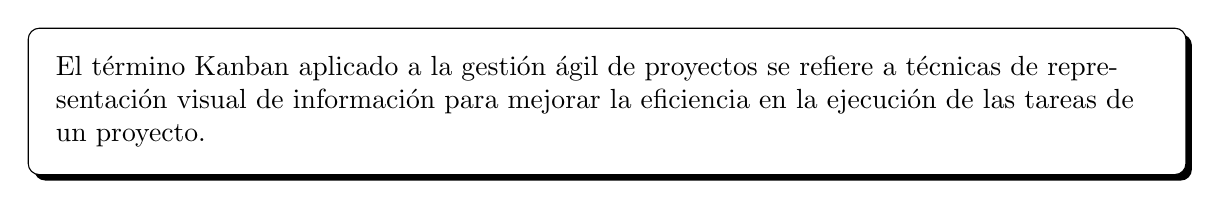
\begin{tikzpicture}
	\node[shadowBox] {
	El término Kanban aplicado a la gestión ágil de proyectos se refiere a técnicas de representación visual de información para mejorar la eficiencia en la ejecución de las tareas de un proyecto.};
\end{tikzpicture}

Kanban se basa en un sistema de producción que dispara el trabajo sólo cuando existe capacidad real para procesarlo \cite{Bahi11}. Este disparador está representado por las tarjetas Kanban, que están limitadas en número. Cada tarjeta representa un trabajo a realizar durante todo el proceso de desarrollo. Al llegar a la última fase, la tarjeta queda liberada para representar un nuevo trabajo.

Kanban mantiene únicamente tres reglas de funcionamiento, mostrar el proceso, limitar el trabajo en curso y optimizar el flujo de trabajo.

	\subsection{Mostrar el proceso}
	Consiste en la visualización de todo el proceso de desarrollo mediante un tablero físico o un tablero virtual accesible por todas las partes, como es el caso de \href{https://trello.com/}{Trello}. El objetivo de este tablero es mejorar el entendimiento del proceso de trabajo actual, anticipar los posibles problemas y ayudar a la toma de decisiones resolutivas.
	Los tableros Kanban están formados por tres secciones, tal y como podemos ver en la figura \ref{fig:kanban_table_1}, \textit{To Do}, \textit{Doing} y \textit{Done}, que corresponden a la pila de entrada, el \ac{WIP} y la salida. Estas secciones se dividen en columnas representativas de los procesos de trabajo. En la figura \ref{fig:kanban_table_2} podemos ver un tablero típico con la pila de entrada (pending) y el \ac{WIP} (analysis, development, test y deploy).
	
	\begin{figure}[H]
	\centering
	\includegraphics[width=120mm, fbox={\fboxrule} 4mm]{images/04-metodo/02-kanban_table_1.png}
	\caption{Secciones tablero Kanban}
	\label{fig:kanban_table_1}
	\end{figure}
	
	\begin{figure}[H]
	\centering
	\includegraphics[width=120mm, fbox={\fboxrule} 4mm]{images/04-metodo/03-kanban_table_2.png}
	\caption{Columnas tablero Kanban}
	\label{fig:kanban_table_2}
	\end{figure}
	
	\subsection{Limitar el trabajo}
	Consiste en limitar la cantidad de ítems o tarjetas que pueden abordarse al mismo tiempo para un proceso definido, es decir, las columnas del tablero. Esta cantidad puede ser visualizada añadiendo el número máximo de tarjetas permitidas a cada columna como un número entre paréntesis al lado del nombre del proceso.
	Esta regla es muy útil para detectar rápidamente los posibles cuellos de botella que puedan producirse. En la imagen \ref{fig:kanban_table_3} podemos observar un desarrollo con un cuello de botella en el proceso \textit{Pruebas}.
	
	\begin{figure}[H]
	\centering
	\includegraphics[width=120mm, fbox={\fboxrule} 4mm]{images/04-metodo/04-kanban_table_3.jpg}
	\caption{Cuello de botella en Kanban}
	\label{fig:kanban_table_3}
	\end{figure}



\section{Marco tecnológico}
En esta sección se incluyen las herramientas y tecnologías utilizadas para el desarrollo del \ac{TFG}.

	\subsection{Sistema Operativo}
		\subsubsection{Elementary OS}
			El sistema operativo utilizado para el desarrollo del proyecto es \textit{\href{https://elementary.io/}{Elementary OS}}. Elementary	es un sistema operativo basado en Ubuntu, a su vez basado en Debian que usa como entorno de escritorio \ac{GNOME}. Al estar basada en Ubuntu es completamente compatible con los repositorios y paquetes de este sistema hasta el punto de usar el \textit{Centro de Software de Ubuntu}.
			Uno de los puntos más fuertes de esta distribución es su gran estabilidad y la interfaz amigable y visualmente atractiva que presenta. Actualmente, este sistema operativo ha sido descargado cinco millones de veces \cite{Garc15}, lo que supone una quinta parte de las descargas totales de la distribución madre (Ubuntu) y existen unos 400.000 usuarios activos \cite{Agud15}.	
	
	\begin{figure}[H]
	\centering
	\includegraphics[width=120mm, fbox={\fboxrule} 4mm]{images/04-metodo/11-elementary_preview.png}
	\caption{Previsualización de Elementary OS}
	\label{fig:elementary-preview}
	\end{figure}
	
	\begin{figure}[H]
	\centering
	\includegraphics[width=40mm, fbox={\fboxrule} 4mm]{images/04-metodo/12-elementary_logo.jpg}
	\caption{Logo Elementary OS}
	\label{fig:elementary-logo}
	\end{figure}
	
			\subsubsection{Microsoft Windows 10}
			Este sistema operativo se utilizará de manera auxiliar debido a que algunas de las herramientas software utilizadas únicamente están disponibles para sistemas operativos Windows.
			La versión 10 del sistema operativo de Microsoft devuelve el protagonismo a los teclados y ratones, perdido en la versión 8 y recuperado parcialmente en la versión 8.1. También destacable es la vuelta del menú inicio a través del conocido botón en la esquina inferior derecha.
			
			\begin{figure}[H]
			\centering
			\includegraphics[width=40mm, fbox={\fboxrule} 4mm]{images/04-metodo/13-windows_logo.png}
			\caption{Logo Microsoft Windows 10}
			\label{fig:windows-logo}
			\end{figure}
			

	\subsection{Herramientas de diseño}
		\subsubsection{Visual Paradigm}
		Visual Paradigm es una herramienta \ac{UML} \ac{Case} para el modelado de sistemas con soporte para \ac{UML} 2.
		Esta herramienta se utilizará para el modelado de los diagramas \ac{UML} necesarios para la consecución del \ac{TFG}.
		Las principales características de esta aplicación son la creación de modelos \ac{UML} con compatibilidad con la versión 2.1 del lenguaje de modelado, el modelado de bases de datos, la interoperabilidad con intercambio de modelos con otras herramientas, el modelado de requerimientos y la generación automática de código y documentación.
		
		\begin{figure}[H]
		\centering
		\includegraphics[width=40mm, fbox={\fboxrule} 4mm]{images/04-metodo/14-visual_paradigm_logo.jpg}
		\caption{Logo Visual Paradigm}
		\label{fig:visual-paradigm-logo}
		\end{figure}
		
		\subsubsection{Gantt Project}
		Es una herramienta utilizada para la creación de diagramas de Gantt, lo que permitirá planificar y organizar el trabajo necesario para la consecución del \ac{TFG}.
		Sus principales características son la posibilidad de importar y exportar archivos de Microsoft Project, la creación de diagramas PERT y la exportación a archivos \ac{PNG}, \ac{PDF} y \ac{HTML},
		
		\begin{figure}[H]
		\centering
		\includegraphics[width=40mm, fbox={\fboxrule} 4mm]{images/04-metodo/15-gantt_project_logo.png}
		\caption{Logo Gantt Project}
		\label{fig:gantt-project-logo}
		\end{figure}
		
		\subsubsection{Moqups}		
		\href{https://moqups.com}{Moqups} es una herramienta online utilizada para la realización de bocetos, maquetación y prototipados rápidos. Su gran ventaja es la cantidad de herramientas que dispone así como el número de plantillas y formas predeterminadas.
			
		\begin{figure}[H]
		\centering
		\includegraphics[width=40mm, fbox={\fboxrule} 4mm]{images/04-metodo/16-moqups_logo.png}
		\caption{Logo Moqups}
		\label{fig:moqups-logo}
		\end{figure}
		
		\begin{figure}[H]
		\centering
		\includegraphics[width=120mm, fbox={\fboxrule} 4mm]{images/04-metodo/17-moqups_preview.jpg}
		\caption{Previsualización Moqups}
		\label{fig:moqups-preview}
		\end{figure}
		
	\subsection{Herramientas de gestión del proyecto}
		\subsubsection{Git}
		Git es un software de control de versiones diseñado por el también creador de Linux, Linus Torvalds. El control de versiones consiste en la gestión y administración de los cambios realizados sobre los archivos involucrados en el desarrollo del presente \ac{TFG}. Permite conocer el estado del proyecto, los cambios que se han realizado, quién los realizó y en qué momento lo hizo y hacer una regresión completa a cualquier estado anterior entre otras características.
		Git es uno de los gestores de control de versiones más conocidos y utilizados, junto con \textit{\ac{SVN}} y \textit{Mercurial}.
		
		\begin{figure}[H]
		\centering
		\includegraphics[width=40mm, fbox={\fboxrule} 4mm]{images/04-metodo/18-git_logo.png}
		\caption{Logo Git}
		\label{fig:git-logo}
		\end{figure}
		
		\subsubsection{Github}
		\label{subsubsection:github}
		Github es un servicio de alojamiento gratuito de repositorios git. En la versión gratuita todos los proyectos son públicos y se hace necesario el contrato de un plan de pago para poder configurar un acceso privado.
		Git y Github son utilizados en el presente \ac{TFG} para establecer un control de versiones en línea, de manera que la comunicación en cuanto a código operativo entre el director y el autor del \ac{TFG}, sea lo más fluida posible.
		
		\begin{figure}[H]
		\centering
		\includegraphics[width=40mm, fbox={\fboxrule} 4mm]{images/04-metodo/19-github_logo.jpg}
		\caption{Logo Github}
		\label{fig:github-logo}
		\end{figure}
	
		\subsubsection{Trello}
		\label{subsubsection:trello}
		Trello es una herramienta colaborativa utilizada para organizar proyectos mediante tableros. Es ampliamente utilizada en el ámbito empresarial para organizar el trabajo a realizar. Debido a sus particularidades, Trello se sincroniza perfectamente con el método Kanban. En el presente \ac{TFG} se utilizará para la ordenación de trabajo y el seguimiento necesario por parte del director hacia el autor.
		
		\begin{figure}[H]
		\centering
		\includegraphics[width=120mm, fbox={\fboxrule} 4mm]{images/04-metodo/20-trello_preview.png}
		\caption{Previsualización de Trello}
		\label{fig:trello-preview}
		\end{figure}
		
		\begin{figure}[H]
		\centering
		\includegraphics[width=40mm, fbox={\fboxrule} 4mm]{images/04-metodo/21-trello_logo.jpg}
		\caption{Logo Trello}
		\label{fig:trello-logo}
		\end{figure}
		
	\subsection{Herramientas, tecnologías y frameworks para el desarrollo}
		\subsubsection{Ruby}
		Ruby es un lenguaje de programación orientado a objetos creado por Yukihiro Matsumoto, también conocido como \textit{Matz}. La principal característica que posee es que absolutamente todo es un objeto, incluso aquello que en otros lenguajes se define como \textit{tipos primitivos}. Al crear el lenguaje, \textit{Matz} se inspiró en Python y Perl intentando que el protagonismo sea la diversión y la productividad del desarrollador \cite{Yuki20}, enfatizando el hecho de que el diseño de sistemas debe prestar más atención a las necesidades humanas que a las necesidades de las máquinas.
		
		\begin{figure}[H]
		\centering
		\includegraphics[width=40mm, fbox={\fboxrule} 4mm]{images/04-metodo/06-ruby_logo.png}
		\caption{Logo Ruby}
		\label{fig:ruby-logo}
		\end{figure}
		
		\subsubsection{Rails}
		Rails es un framework de desarrollo web escrito en Ruby siguiendo el paradigma \ac{MVC} (ver figura \ref{fig:mvc}). Se basa en dos principios fundamentales, \textit{\ac{DRY}} (no te repitas), esto es, escribir el mismo código una y otra vez es una mala praxis y \textit{Convención sobre Configuración} que permite que Rails suponga que quieres hacer y como quieres hacerlo en función de las prácticas habituales de programación. Se utilizará para el desarrollo de la herramienta web.
		
		\begin{figure}[h!btp]
		\centering
		\includegraphics[width=120mm, fbox={\fboxrule} 4mm]{images/04-metodo/07-mvc.jpg}
		\caption{Modelo Vista Controlador}
		\label{fig:mvc}
		\end{figure}
		
		\begin{figure}[H]
		\centering
		\includegraphics[width=40mm, fbox={\fboxrule} 4mm]{images/04-metodo/08-rails_logo.png}
		\caption{Logo Rails}
		\label{fig:rails-logo}
		\end{figure}
		
		\subsubsection{Android}
		Android es un sistema operativo desarrollado inicialmente para móviles que utiliza los kernel de Linux como núcleo del mismo. Durante el año 2014 alcanzó una cuota de mercado del 63 \% (ver figura \ref{fig:os-mobile}. Fuente \cite{Are15})por lo que puede considerarse el más importante de los sistemas operativos móviles. 
		La aplicación móvil se desarrollará para este sistema operativo, utilizando para ello el lenguaje Java.
		
		\begin{figure}[h!btp]
		\centering
		\includegraphics[width=60mm, fbox={\fboxrule} 4mm]{images/04-metodo/09-os_mobile.png}
		\caption{Cuota de mercado de los sistemas operativos móviles}
		\label{fig:os-mobile}
		\end{figure}
		
		\begin{figure}[H]
		\centering
		\includegraphics[width=40mm, fbox={\fboxrule} 4mm]{images/04-metodo/10-android_java.jpg}
		\caption{Logo Android y Java}
		\label{fig:android-java-logo}
		\end{figure}

		\subsubsection{Bootstrap}
		Bootstrap es un framework \ac{CSS} desarrollado en el año 2011 por Twitter. El código fue liberado y actualmente está accesible en Github. Permite la creación de interfaces limpias y funcionales y mantiene un diseño \textit{responsive} o adaptativo, esto es, adopta automáticamente el tamaño adecuado al dispositivo en el que debe mostrarse la vista.
		
		\begin{figure}[H]
		\centering
		\includegraphics[width=40mm, fbox={\fboxrule} 4mm]{images/04-metodo/23-bootstrap_logo.png}
		\caption{Logo Bootstrap}
		\label{fig:bootstrap-logo}
		\end{figure}
		
		\begin{figure}[H]
		\centering
		\includegraphics[width=120mm, fbox={\fboxrule} 4mm]{images/04-metodo/24-bootstrap_preview.jpg}
		\caption{Previsualización de Bootstrap}
		\label{fig:bootstrap-preview}
		\end{figure}
		
		\subsubsection{Rspec}
		Rspec es una librería para Ruby diseñada para la realización de pruebas. Actualmente es una de las herramientas más populares para este cometido en Ruby. Su diseño está enfocado tanto a la productividad como a la comodidad y diversión del desarrollador.

		\begin{figure}[H]
		\centering
		\includegraphics[width=40mm, fbox={\fboxrule} 4mm]{images/04-metodo/25-rspec_logo.png}
		\caption{Logo Rspec}
		\label{fig:rspec-logo}
		\end{figure}
		
		\subsubsection{\ac{HTML}}
		\ac{HTML} es un lenguaje de marcado utilizado para la creación y diseño de páginas web. Es un estándar a cargo de \ac{W3C}. La interpretación del código corre a cargo del navegador web. En octubre de 2014 se publicó la versión definitiva de la nueva revisión, \ac{HTML}5.
		
		\begin{figure}[H]
		\centering
		\includegraphics[width=40mm, fbox={\fboxrule} 4mm]{images/04-metodo/26-html_logo.png}
		\caption{Logo HTML5}
		\label{fig:html5-logo}
		\end{figure}
		
		\subsubsection{\ac{CSS}}
		Es un mecanismo para describir cómo va a mostrarse un documento, ofreciendo a los desarrolladores el control sobre el formato de los documentos. Se utiliza para concretar el estilo de los documentos \ac{HTML}. Actualmente está en su tercera versión, \ac{CSS}3.

		\begin{figure}[H]
		\centering
		\includegraphics[width=40mm, fbox={\fboxrule} 4mm]{images/04-metodo/27-css3_logo.png}
		\caption{Logo CSS3}
		\label{fig:css3-logo}
		\end{figure}	
		
		\subsubsection{\ac{JSON}}
		\ac{JSON} es un formato para el intercambio de datos nacido como alternativa a \ac{XML}. Una de sus mayores ventajas es que puede leerse con cualquier lenguaje de programación, por lo que es usado para el intercambio de información entre distintos sistemas. El funcionamiento básico para formar estructuras de datos válidas, es mediante pares clave-valor.
		
		\begin{figure}[H]
		\centering
		\includegraphics[width=40mm, fbox={\fboxrule} 4mm]{images/04-metodo/28-json_logo.png}
		\caption{Logo JSON}
		\label{fig:json-logo}
		\end{figure}	
		
		\subsubsection{Sublime Text 3}
		\textit{Sublime Text 3} es un editor de texto y código fuente escrito en \textit{C++}. Originalmente era una extensión de \textit{Vim}, que a su vez es una versión mejorada de \textit{Vi}, un editor de texto presente en los sistemas UNIX.
		Este programa será el utilizado para la escritura del código necesario durante la elaboración del \ac{TFG}.
		
		\begin{figure}[H]
		\centering
		\includegraphics[width=40mm, fbox={\fboxrule} 4mm]{images/04-metodo/29-sublime_text_logo.png}
		\caption{Logo Sublime Text 3}
		\label{fig:sublime-text-logo}
		\end{figure}
		
		\subsubsection{Midori}
		Es el navegador web por defecto de Elementary OS con un motor principal basado en Webkit, conocido por la estabilidad de los navegadores Safati, Chrome y Opera. Se utilizará para el acceso a la aplicación web. Debido a que usa \ac{GTK} como interfaz gráfica puede ejecutarse sin errores en escritorios basados en \ac{GNOME} o Xfce.
		Ofrece compatibilidad con HTML5 y CSS3.
		
		\begin{figure}[H]
		\centering
		\includegraphics[width=40mm, fbox={\fboxrule} 4mm]{images/04-metodo/30-midori_logo.png}
		\caption{Logo Midori}
		\label{fig:midori-logo}
		\end{figure}
		
		\subsubsection{Chromium}
		Es un navegador web de código abierto basado en Google Chrome.
		Tiene un diseño minimalista y su motor principal está basado en Webkit. La mayor parte de este proyecto está bajo licencia BSD, lo que permite el uso parcial o total de su código fuente. Su punto fuerte consiste en su estabilidad, debido a que usa un proceso para cada pestaña, el bloqueo de uno de ellos no afecta al funcionamiento general del programa.
		Ofrece compatibilidad con HTML5 y CSS3.
		
		\begin{figure}[H]
		\centering
		\includegraphics[width=40mm, fbox={\fboxrule} 4mm]{images/04-metodo/39-chromium_logo.png}
		\caption{Logo Chromium}
		\label{fig:chromium-logo}
		\end{figure}
		
		\subsubsection{Mozilla Firefox}		
		Es uno de los navegadores más conocidos y usados, junto con Internet Explorer y Google Chrome, está desarrollado mediante una licencia de código abierto.
		Es compatible con los principales lenguajes de programación web y destaca su velocidad y estabilidad.

		\begin{figure}[H]
		\centering
		\includegraphics[width=40mm, fbox={\fboxrule} 4mm]{images/04-metodo/38-firefox_logo}
		\caption{Logo Mozilla Firefox}
		\label{fig:firefox-logo}
		\end{figure}
		
	\subsection{Herramientas para la gestión de bases de datos}
		\subsubsection{MongoDB}
		Es una base de datos NoSQL orientada a documentos, esto es, en vez de guardar los datos en registros los guarda en documentos en una representación binaria de \ac{JSON} conocida como \ac{BSON}. La principal diferencia con las bases de datos relacionales, es que no resulta necesario seguir un mismo esquema para una misma colección (concepto similar a las tablas de las bases de datos relacionales).
		
		\begin{figure}[H]
		\centering
		\includegraphics[width=40mm, fbox={\fboxrule} 4mm]{images/04-metodo/31-mongodb_logo.png}
		\caption{Logo MongoDB}
		\label{fig:mongodb-logo}
		\end{figure}	
		
		\subsubsection{MongoLab}
		MongoLab nos permite el uso de una base de datos como servicio \ac{SaaS}, usando para ello la infraestructura proporcionada por distintos proveedores como Google, Amazon o Microsoft.
				
		\begin{figure}[H]
		\centering
		\includegraphics[width=40mm, fbox={\fboxrule} 4mm]{images/04-metodo/33-mongolab-logo.png}
		\caption{Logo MongoLab}
		\label{fig:mongolab-logo}
		\end{figure}
		
		\subsubsection{MongoChef}
		MongoChef es un administrador gráfico de bases de datos MongoDB que permite mantener múltiples conexiones a las bases de datos, bien a través del servidor local, bien a través de MongoLab.
		
		\begin{figure}[H]
		\centering
		\includegraphics[width=40mm, fbox={\fboxrule} 4mm]{images/04-metodo/32-mongochef_logo.png}
		\caption{Logo MongoChef}
		\label{fig:mongochef-logo}
		\end{figure}
	
	\subsection{Herramientas documentales}
		\subsubsection{TexMaker}
		TexMaker es un editor gráfico para lenguaje LaTex distribuido bajo licencia \textit{\ac{GPL}}. Existen versiones disponibles para Microsoft Windows, Linux / Unix y Mas OsX. Permite la edición de texto automático mediante asistentes configurables y la detección y manejo de los errores de manera rápida y sencilla.
				
		\begin{figure}[H]
		\centering
		\includegraphics[width=40mm, fbox={\fboxrule} 4mm]{images/04-metodo/34-texmaker_logo.png}
		\caption{Logo Texmaker}
		\label{fig:texmaker-logo}
		\end{figure}
		
		\subsubsection{\ac{GIMP}}
		\ac{GIMP} es un editor de imágenes tanto en mapa de bits como en dibujos y fotografías, libre y gratuito. Forma parte del proyecto \ac{GNU} y se publica bajo la misma licencia. Es uno de los programas de manipulación de gráficos más utilizado y probablemente el más usado en entornos GNU / Linux. Se utilizará para la modificación, edición y creación de imágenes para el presente \ac{TFG}.
		
		\begin{figure}[H]
		\centering
		\includegraphics[width=40mm, fbox={\fboxrule} 4mm]{images/04-metodo/35-gimp_logo.png}
		\caption{Logo \ac{GIMP}}
		\label{fig:gimp-logo}
		\end{figure}
		
		\subsubsection{Microsoft Visio}
		Es un software de dibujo vectorial para el sistema operativo Windows que permite la realización de diversos tipos de diagramas. 
		
		\begin{figure}[H]
		\centering
		\includegraphics[width=40mm, fbox={\fboxrule} 4mm]{images/04-metodo/36-visio_logo.jpg}
		\caption{Logo Microsoft Visio}
		\label{fig:visio-logo}
		\end{figure}
	
	\subsection{Herramientas de implantación}
		\subsubsection{Heroku}
		\label{subsubsection:heroku}
		Heroku es un servicio \ac{PaaS} utilizado para el despliegue de aplicaciones en línea desarrolladas, entre otros lenguajes, en Ruby.
				
		\begin{figure}[H]
		\centering
		\includegraphics[width=40mm, fbox={\fboxrule} 4mm]{images/04-metodo/37-heroku_logo.png}
		\caption{Logo Heroku}
		\label{fig:heroku-logo}
		\end{figure}
	

% Local Variables:
%  coding: utf-8
%  mode: latex
%  mode: flyspell
%  ispell-local-dictionary: "castellano8"
% End:

\chapter{Resultados}
\label{chap:resultados}

% Referencias a documentos externos
\externaldocument{metodo}

\drop{E}{n} este capítulo se muestran los resultados obtenidos para la consecución del presente \ac{TFG}. La estructura del capítulo se basa en las iteraciones propias de la metodología elegida y definida en la sección 4 (ver sección \ref{section:desarrollo}). Es necesario llevar a cabo un sprint 0 que servirá para detallar los apartados principales de la gestión del mismo, como los requisitos y el alcance del proyecto, las historias de usuario, la gestión temporal, gestión de usuarios y riesgos y otras acciones necesarias.

Debido al carácter académico del proyecto, los recursos y la gestión de los mismos estarán alejados de los parámetros habituales del mercado laboral, ya que todos los roles necesarios serán desarrollados por dos personas, el autor y el director del proyecto.

\section{Sprint 0}
Esta primera iteración tiene como objetivo definir el alcance del proyecto y su realizar la planificación del mismo, de manera que quede definida una sólida base sobre la que comenzar el desarrollo del mismo. Se estimará el coste temporal y económico, y se abordará la planificación de los recursos que se consideran necesarios para la correcta consecución de los objetivos planteados, tanto técnicos como humanos, y la gestión de los mismos que se pretende llevar a cabo.

	\subsection{Gestión de recursos humanos}
	Tal y como se comentó en la introducción al capítulo, las personas involucradas en el desarrollo del proyecto son el autor y el director del mismo, que coparán todos los roles disponibles, quedando estos de la siguiente manera:
	
	\begin{itemize}[label={$\bullet$},labelindent=\parindent,leftmargin=2cm]
		\item Autor del \ac{TFG}: Equipo de desarrollo, análisis y pruebas del producto.
		\item Director del \ac{TFG}: Propietario, usuario y cliente final del producto.
	\end{itemize}
	
	\subsection{Alcance del proyecto}
		\subsubsection{Descripción del alcance}
		\label{subsubsection:descripcion-alcance}
		El proyecto consistirá en la elaboración de una herramienta accesible a través de una página web, asimismo se proporcionará una aplicación móvil para sistemas operativos Android que facilitará el acceso a la mencionada página.
		\\La página constará de dos secciones delimitadas por los privilegios necesarios de acceso. 
		
		Una primera sección de acceso libre en la que se encuadran las páginas \textit{Inicio}, \textit{Acerca de}, \textit{Contacto} y aquellas páginas auxiliares necesarias para permitir el registro y autenticación a los usuarios que deseen acceder a la segunda sección.
		\\Para ganar acceso a la segunda sección será necesario autentificarse mediante un usuario y una contraseña adquiridos mediante un formulario de registro. Esta sección englobará las páginas de gestión de los datos personales del usuario y el acceso a las posiciones geográficas guardadas para este usuario.
		\\La herramienta permitirá al usuario definir una localización geográfica como posición de aparcamiento de su vehículo seleccionando la ubicación mediante un mapa interactivo.
		La herramienta mostrará al usuario la localización actual de los elementos guardados previamente mediante un mapa interactivo.
		\\Los usuarios podrán permitir la compartición de la localización de un elemento con otros usuarios legítimos de la herramienta, llamados \textit{usuarios secundarios}.
		\\Los \textit{usuarios secundarios} podrán modificar los elementos compartidos bajo las mismas condiciones que el \textit{usuario primario} o usuario propietario del elemento.
		\\El \textit{usuario primario} podrá revocar los derechos de acceso y edición a los \textit{usuarios secundarios}.
		La herramienta estará diseñada para facilitar el acceso a través de dispositivos móviles mediante los navegadores incorporados.
		\\Se pondrá a disposición de los usuarios con sistemas operativos Android una aplicación que permitirá el acceso rápido a la herramienta web.
	
		\subsubsection{Criterios de aceptación}
		\label{subsubsection:criterios-aceptacion}
		La herramienta se considerará conforme a criterio siempre que cumpla los puntos detallados a continuación.
		
		\begin{itemize}[label={$\bullet$},labelindent=\parindent,leftmargin=2cm]
			\item La herramienta web debe visualizarse correctamente en los navegadores Midori, Chromium,Chrome y Mozilla Firefox.
			\item La aplicación debe dar acceso a la herramienta web y permitir una correcta visualización de la misma.
			\item La herramienta web debe garantizar el acceso mediante autenticación a los usuarios legítimos, impidiendo el acceso a la sección restringida a los usuarios no identificados.
			\item La herramienta web debe contener mecanismos para el alta de nuevos usuarios y contendrá mecanismos para la recuperación de los datos de entrada por parte de los usuarios legítimos.
			\item La herramienta mostrará un mapa interactivo en el que estarán señalados los elementos guardados por el usuario y permitirá la adición de nuevos elementos o la modificación de los existentes.
			\item La herramienta incorporará mecanismos para permitir la compartición de elementos entre usuarios legítimos y para revocar está compartición.
			\item La herramienta permitirá a los \textit{usuarios secundarios} modificar los elementos compartidos con ellos por los \textit{usuarios primarios}.
			\item La herramienta permitirá a los \textit{usuarios primarios} revocar los derechos de visión y edición de los \textit{usuarios secundarios} a los elementos previamente compartidos.
		\end{itemize}

		\subsubsection{Entregables del proyecto}
		Al finalizar cada una de las iteraciones se entregará al cliente un artefacto en forma de página de web con las características añadidas a la herramienta durante la iteración así como la documentación generada durante esta fase.
		
	Al termino de las iteraciones se entregará la herramienta completa según lo descrito en la descripción del alcance (ver descripción del alcance \ref{subsubsection:descripcion-alcance}) conforme a criterios (ver criterios \ref{subsubsection:criterios-aceptacion}), un manual de usuario de la herramienta, un manual de instalación y una memoria con los documentos generados durante el proceso de desarrollo.
	
		\subsubsection{Suposiciones y restricciones del proyecto}
		Para asegurar el correcto funcionamiento de la herramienta debe tenerse en cuenta los puntos descritos a continuación:
		
		\begin{itemize}[label={$\bullet$},labelindent=\parindent,leftmargin=2cm]
			\item Se asegura el correcto funcionamiento al acceder desde los siguientes navegadores: Midori, Chromium, Chrome y Mozilla Firefox.
			\item La aplicación móvil será compatible con versiones Android 4.1 y posteriores.
		\end{itemize}

	\subsection{Plan del proyecto}
	En función de los requisitos del proyecto, definidos en la sección \textit{Objetivos} \ref{chap:objetivos} y teniendo en cuenta el alcance del proyecto (ver subsección \ref{subsubsection:descripcion-alcance}) y los criterios de aceptación del mismo (ver subsección \ref{subsubsection:criterios-aceptacion}) se puede crear la pila de producto, que consistirá en una colección de \textit{historias de usuario} del sistema, su valor de negocio y la estimación temporal para llevarlo a cabo. Tanto el valor de negocio como la estimación han sido llevadas a cabo contando con la ayuda del propietario del producto.
	En la tabla \ref{tab:historia_usuario} podemos observar las historias de usuario retratadas en una pila de producto priorizada en la que se incluye una estimación temporal y el valor de negocio considerado para la misma.


	\begin{longtable}{p{2cm} p{6cm} p{4cm} p{3cm}}
	  	\hline
  	    \multicolumn{1}{p{2cm}}{\cellcolor{black!30}\textbf{Id}} &
	    \multicolumn{1}{p{6cm}}{\cellcolor{black!30}\textbf{Historia de Usuario}} & 
	 	\multicolumn{1}{p{4cm}}{\cellcolor{black!30}\textbf{Estimación temporal}} &
 	 	\multicolumn{1}{p{3cm}}{\cellcolor{black!30}\textbf{Valor de negocio}}
	 	\\
	 	\toprule 
	   % \toprule
	   	\endfirsthead
	     
	    \hline
  	    \multicolumn{1}{p{2cm}}{\cellcolor{black!30}\textbf{Id}} &
	    \multicolumn{1}{p{6cm}}{\cellcolor{black!30}\textbf{Historia de Usuario}} & 
	 	\multicolumn{1}{p{4cm}}{\cellcolor{black!30}\textbf{Estimación temporal}} &
 	 	\multicolumn{1}{p{3cm}}{\cellcolor{black!30}\textbf{Valor de negocio}}
	 	\\	 
	 	\toprule
	 	\endhead	

		\rowcolor{gray!25}
		HdU 1	&	Como cliente quiero que los usuarios se registren antes de acceder a la aplicación y a sus datos	
				&	20 horas		&	Alto	\\
		HdU 2	&	Como usuario quiero acceder mediante un nombre y una contraseña para que sólo yo pueda entrar a mi cuenta							&	10 horas	&	Alto	\\
		\rowcolor{gray!25}
		HdU 3	&	Como usuario quiero modificar mis datos guardados	o eliminar mi cuenta												
				&	12 horas	&	Alto	\\ 
		HdU 4	& 	Como usuario quiero guardar mis ubicaciones mediante un mapa para poder acceder a ellas más tarde	
				&	30 horas	&	Alto	\\
		\rowcolor{gray!25}
		HdU 5	&	Como usuario quiero recuperar todas mis ubicaciones guardadas, verlas dibujadas en un mapa y ver el nombre y el número de la calle donde están aparcados
				&	12 horas	&	Alto	\\
		HdU 6	&	Como usuario quiero recuperar y ver en el mapa una de mis ubicaciones guardadas, también quiero ver la dirección postal completa
				&	10 horas	&	Alto	\\
		\rowcolor{gray!25}
		HdU 7	&	Como usuario quiero poder añadir mis coches para poder guardar su ubicación															&	12 horas	&	Alto	\\
		HdU 8	&	Como usuario quiero poder borrar o editar los datos guardados de mis coches
				&	12 horas	&	Medio	\\	
		\rowcolor{gray!25}
		HdU 9	&	Como usuario quiero compartir mis ubicaciones guardadas con otros usuarios de mi elección para que puedan modificarlas			
				&	30 horas&	Medio	\\
		HdU 10	&	Como usuario quiero dejar de compartir mis ubicaciones guardadas con otros usuarios de mi elección para que puedan modificarlas			
				&	10 horas&	Medio	\\
		\rowcolor{gray!25}
		HdU 11	&	Como usuario quiero que la aplicación me muestre la ruta a pie desde mi posición actual hasta la ubicación seleccionada
				&	6 horas	&	Bajo	\\
	    \hline
	  \caption{Objetivos parciales del \ac{TFG}}
	  \label{tab:historia_usuario}
	\end{longtable}

Una vez tenemos la lista de producto priorizada podemos dividir el trabajo en los distintos sprint que generarán como resultado la consecución de los objetivos marcados. En las tablas \ref{tab:plan_proyecto} y \ref{tab:validaciones_HdU} podemos observar la división realizada, los artefactos resultantes y la validación necesaria para lograr el objetivo marcado.

\begin{longtable}{p{1cm} p{4cm} p{4cm} p{6cm}}
  	\hline  	    
  	\multicolumn{1}{p{1cm}}{\cellcolor{black!30}\textbf{Sprint}} &
    \multicolumn{1}{p{4cm}}{\cellcolor{black!30}\textbf{Historia de Usuario}} & 
 	\multicolumn{1}{p{4cm}}{\cellcolor{black!30}\textbf{Estimación temporal}} &
 	\multicolumn{1}{p{6cm}}{\cellcolor{black!30}\textbf{Artefactos}}
 	\\
 	\toprule 
   % \toprule
   	\endfirsthead
     
    \hline
  	\multicolumn{1}{p{1cm}}{\cellcolor{black!30}\textbf{Sprint}} &
    \multicolumn{1}{p{4cm}}{\cellcolor{black!30}\textbf{Historia de Usuario}} & 
 	\multicolumn{1}{p{4cm}}{\cellcolor{black!30}\textbf{Estimación temporal}} &
 	\multicolumn{1}{p{6cm}}{\cellcolor{black!30}\textbf{Artefactos}}
 	\\	 
 	\toprule
 	\endhead

	\rowcolor{gray!25}
	1	& HdU 1, HdU 2 y HdU 3	&	42 horas	&	Prototipo de página web con autenticación, edición y administración de usuarios \\ 
	2	& HdU 5					&	12 horas	&	Prototipo que muestre en un mapa una serie de ubicaciones geográficas guardadas previamente y sus correspondientes direcciones postales mediante un texto \\
	\rowcolor{gray!25}
	3	& HdU 4				&	30 horas	&	Prototipo que guarde una ubicación geográfica elegida por el usuario mediante la interacción con un mapa \\
	4	& HdU 7					&	12 horas	&	Prototipo que permite crear nuevos elementos para almacenar la ubicación geográfica del mismo y muestra la ubicación de un elemento seleccionado \\
	\rowcolor{gray!25}
	5	& HdU 6					& 	10 horas	& 	Prototipo que muestra en un mapa la posición de un elemento seleccionado y su correspondiente dirección postal mediante texto\\
	6	& HdU 8					&	12 horas	&	Prototipo que permite modificar o borrar los datos almacenados de los elementos a mostrar \\
	\rowcolor{gray!25}
	7	& HdU 9 y HdU 10		&	40 horas	&	Prototipo que permite compartir la ubicación de los elementos almacenados con otros usuarios válidos del sistema y revocar este permiso \\
	8	& HdU 11				&	6 horas		&	Prototipo que muestra la ruta a pie desde la posición actual del usuario hasta el elemento seleccionado \\

	\hline
	\caption{Plan de proyecto detallado}
	\label{tab:plan_proyecto}
\end{longtable}

\begin{longtable}{p{1cm} p{4cm} p{4cm} p{6cm}}
  	\hline  	    
  	\multicolumn{1}{p{1cm}}{\cellcolor{black!30}\textbf{Sprint}} &
    \multicolumn{1}{p{4cm}}{\cellcolor{black!30}\textbf{Historia de Usuario}} & 
 	\multicolumn{1}{p{4cm}}{\cellcolor{black!30}\textbf{Estimación temporal}} &
 	\multicolumn{1}{p{6cm}}{\cellcolor{black!30}\textbf{Validación}}
 	\\
 	\toprule 
   	\endfirsthead
	%\multirow{3}{4cm}{multifila 1-3} &
	     
    \hline
  	\multicolumn{1}{p{1cm}}{\cellcolor{black!30}\textbf{Sprint}} &
    \multicolumn{1}{p{4cm}}{\cellcolor{black!30}\textbf{Historia de Usuario}} & 
 	\multicolumn{1}{p{4cm}}{\cellcolor{black!30}\textbf{Estimación temporal}} &
 	\multicolumn{1}{p{6cm}}{\cellcolor{black!30}\textbf{Validación}}
 	\\	 
 	\toprule
 	\endhead

	\rowcolor{gray!25}
	\multirow{3}{*}{1}	& HdU 1	&	20 horas	&	Los usuarios anónimos pueden darse de alta en el sistema. \\ 
	\rowcolor{gray!25}	& HdU 2	&	10 horas	&	Los usuarios anónimos no pueden acceder a la aplicación. Los usuarios registrados 														pueden acceder a la aplicación. \\ 
	\rowcolor{gray!25}	& HdU 3	&	12 horas	&	Los usuarios registrados pueden modificar los datos de su cuenta o darse de baja en 														la aplicación.  \\                      
	
	2	& HdU 5		&	12 horas	&	Los usuarios registrados podrán ver en un mapa las ubicaciones guardadas y en un cuadro de 												texto la dirección postal de la misma.\\
	\rowcolor{gray!25}
	3	& HdU 4		&	30 horas	&	Los usuarios registrados podrán guardar en la base de datos ubicaciones 																	interactuando con el mapa. \\
	
	4	& HdU 7		&	12 horas	&	Los usuarios registrados podrán crear nuevos elementos sobre los que guardar ubicaciones 													geográficas. \\
	\rowcolor{gray!25}
	5	& HdU 6		&	10 horas	&	Los usuarios registrados podrán seleccionar uno de los elementos 																			guardados para mostrar únicamente su ubicación en el mapa. \\

	6	& HdU 8		&	12 horas	&	Los usuarios registrados podrán modificar las propiedades de los elementos que hayan creado o 											borrarlos del sistema. \\
	\rowcolor{gray!25}
	\multirow{2}{*}{7}	& HdU 9		&	30 horas	&	Los usuarios registrados podrán ver y modificar las ubicaciones de los elementos 															previamente compartidos con ellos por otros usuarios registrados. \\
	\rowcolor{gray!25}	& HdU 10	&	10 horas	&	Los usuarios registrados no podrán ver ni modificar las ubicaciones de los 																elementos que hayan dejado de compartirse con ellos por otros usuarios 																	registrados. \\

	8	& HdU 11	&	6 horas		&	Los usuarios registrados podrán ver una ruta a pie desde su ubicación actual hasta la ubicación 											almacenada del elemento seleccionado. \\

	\hline
	\caption{Historias de Usuario y validaciones}
	\label{tab:validaciones_HdU}
\end{longtable}

	\subsection{Gestión temporal del proyecto}
	Una vez definido el alcance del proyecto mediante las historias de usuario y su división en sprint, se realizará un diagrama de Gantt con la estimación temporal del proyecto.
	Como fecha de inicio para el desarrollo, esto es, para el sprint 0 se elige la fecha de 15 de septiembre de 2015 y para la consecución del mismo se estima una duración aproximada de veinticuatro días. La duración de la jornada laboral se fija en 6 horas diarias de lunes a viernes, observando las fechas marcadas como festivo en el calendario laboral general.
	Debido a que el equipo de desarrollo está formado por una única persona, la posibilidad de paralelizar trabajo se ve limitada a la elaboración de la presente memoria al tiempo que se realiza el desarrollo de la aplicación, pero no al desarrollo de historias de usuario simultáneamente.
	Se estima que la realización, revisión y corrección de la memoria necesitará un tiempo total de trabajo de quince días aproximadamente.
	En la figura \ref{fig:gantt} puede observarse el correspondiente diagrama de Gantt de la planificación.

\begin{sidewaysfigure}[h!t]
	\includegraphics[height=80mm, fbox={\fboxrule} 4mm]{./images/05-resultados/01-gantt.png}
	\caption{Diagrama de Gantt del \ac{TFG}}
	\label{fig:gantt}
\end{sidewaysfigure}
	
	\subsection{Gestión de las comunicaciones}
	La comunicación entre el autor del presente \ac{TFG} y el director del proyecto se realizará para la información puntual del estado del desarrollo y abordar las posibles dudas generadas durante el desarrollo. Generalmente las reuniones se realizarán semanalmente y se concretarán, preferentemente, mediante correo electrónico.
	Se utilizarán también otro tipo de herramientas para comunicar en todo momento el estado del proyecto y facilitar la comunicación entre los dos actores principales del desarrollo, a saber, el autor y el director. Estas herramientas serán \textit{Trello}, \textit{Github} y \textit{Heroku}.\\
	Trello, tal y como se explicó anteriormente (ver subsección \ref{subsubsection:trello}) es un tablero Kanban virtual que permitirá al director estar informado en todo momento de las tareas que el autor está llevando a cabo en cada momento, así como la modificación de la lista de tareas si así lo considerase necesario. Para ello se crea y permite el acceso al director a un nuevo tablero Kanban iniciado para el presente proyecto. En la figura \ref{fig:trello} puede observarse una captura de pantalla del panel Kanban en Trello.

\begin{figure}[H]
\centering
\includegraphics[width=17cm, fbox={\fboxrule} 4mm]{images/05-resultados/03-trello.jpg}
\caption{Panel Kamban de Trello}
\label{fig:trello}
\end{figure}
	
	
	Github, tal y como se explicó anteriormente (ver subsección \ref{subsubsection:github}) es un servidor para repositorios \textit{Git} que se utilizará para el almacenaje en línea tanto del código del proyecto como de la memoria del mismo. Debido a las restricciones existentes en el servicio gratuito, el repositorio es público, por lo que únicamente se procederá a informar al director del proyecto de la dirección donde se encuentra almacenado. Mediante estos actos, se conseguirá que el director tenga acceso completo a toda la documentación generada para la consecución del proyecto pudiendo revisarla cuando así lo que creyera necesario. Esto mismo es aplicable al código fuente del presente proyecto. En la figura \ref{fig:github} puede verse una captura de pantalla de algunos commit subidos al repositorio.
	
\begin{figure}[H]
\centering
\includegraphics[width=15cm, fbox={\fboxrule} 4mm]{images/05-resultados/02-git.jpg}
\caption{Commits en repositorio en GitHub}
\label{fig:github}
\end{figure}
	
	Heroku, tal y como se explicó anteriormente (ver subsección \ref{subsubsection:heroku}) es el servidor usado para la implantación del presente proyecto, por lo que se utilizará para comprobar los avances en el proyecto mediante la visita a través de un navegador web.
	
	\subsection{Gestión de recursos}
	Tal y como se comentó anteriormente (ver sección \ref{section:dispositivos-empleados}), para el desarrollo del proyecto se utilizará un equipo con las características detalladas en la tabla \ref{tab:portatil2}. 
	
	\begin{table}[H]
	  \centering 
	  \rowcolors{1}{gray!25}{white}
	  \begin{tabular}{p{0.4\linewidth}p{0.3\linewidth}}
	    \toprule
		Procesador 							& Intel i7-5500U								\\
		Velocidad y Núcleos del Procesador & 2.4 GHz; 2 núcleos 							\\
		Memoria RAM 						& 16 \ac{GB} \ac{DDR}3L \ac{SDRAM} 			\\
		Sistema Operativo					& Elementary \ac{OS} 							\\
	    \hline
	  \end{tabular}
	  \caption{Equipo usado para el desarrollo \ac{TFG}}
	  \label{tab:portatil2}
	\end{table}
	
	Para las pruebas con dispositivos móviles se utilizará un equipo con las características mostradas en la tabla \ref{tab:movil2}.
	\begin{table}[H]
	  \centering 
	  \rowcolors{1}{gray!25}{white}
	  \begin{tabular}{p{0.3\linewidth}p{0.4\linewidth}}
	    \toprule
		Procesador 	& Qualcomm Snapdragon 800		\\
		Velocidad Procesador 	& 2.26 GHz 			\\
		Memoria RAM 			& 2 \ac{GB} 		\\
		Sistema Operativo 		& Android 6.0 		\\
	    \hline
	  \end{tabular}
	  \caption{Equipo usado para las pruebas en dispositivos móviles \ac{TFG}}
	  \label{tab:movil2}
	\end{table}
	
	\subsection{Gestión de riesgos}
	Para la gestión de riesgos del presente proyecto se utiliza una modificación de la lista proporcionada por McConnell en \cite{Mcc97} presentado en la tabla \ref{tab:riesgos}	los riesgos a los que se podría enfrentar el autor durante el desarrollo, mostrando la probabilidad de que sucedan y el retraso producido en caso de ocurrencia.
	
	\begin{longtable}{p{1cm} p{8cm} p{3cm} p{2cm}}
	  	\hline
  	    \multicolumn{1}{p{1cm}}{\cellcolor{black!30}\textbf{Id}} &
	    \multicolumn{1}{p{8cm}}{\cellcolor{black!30}\textbf{Riesgo}} & 
	 	\multicolumn{1}{p{3cm}}{\cellcolor{black!30}\textbf{Probabilidad}} &
 	 	\multicolumn{1}{p{2cm}}{\cellcolor{black!30}\textbf{Retraso}}
	 	\\
	 	\toprule 
	   % \toprule
	   	\endfirsthead
	     
	    \hline
  	    \multicolumn{1}{p{1cm}}{\cellcolor{black!30}\textbf{Id}} &
	    \multicolumn{1}{p{8cm}}{\cellcolor{black!30}\textbf{Riesgo}} & 
	 	\multicolumn{1}{p{3cm}}{\cellcolor{black!30}\textbf{Probabilidad}} &
 	 	\multicolumn{1}{p{2cm}}{\cellcolor{black!30}\textbf{Retraso}}
	 	\\	 
	 	\toprule
	 	\endhead
   	    
		\multicolumn{4}{l}{\cellcolor{gray!25}\textbf{A. Creación de la planificación}}\\
		A.1. &El esfuerzo es mayor que el estimado.											&	40\%	&	7 días	\\
		A.2. &Un retraso en una tarea produce retrasos en cascada en las tareas dependientes 	&	40\%	&	7 días	\\
		
		\multicolumn{4}{l}{\cellcolor{gray!25}\textbf{B. Organización y gestión}}\\
		B.3. &Afectación por el \textit{Síndrome de la hoja en blanco}							&	20\%	&	2 días	\\
		
%		\multicolumn{1}{r}{\cellcolor{black!30}\textbf{C. }} &
		\multicolumn{4}{l}{\cellcolor{gray!25}\textbf{C. Entorno de desarrollo}}\\
		C.4. &Los espacios no están disponibles en el momento necesario						&	60\%	&	24 horas\\
		C.5. &Los espacios están disponibles pero no son adecuados								&	35\%	&	24 horas\\
		C.6. &Los espacios están sobreutilizados, son ruidosos o distraen						&	60\%	&	24 horas\\
		C.7. &La curva de aprendizaje para la nueva herramienta de desarrollo es más larga de lo esperado	&	20\%	&	2 días	\\
		
%%		\multicolumn{1}{r}{\cellcolor{black!30}\textbf{D. }} &
		\multicolumn{4}{l}{\cellcolor{gray!25}\textbf{D. Usuarios finales}}\\
		&No aplicable&&\\
		
%		\multicolumn{1}{r}{\cellcolor{black!30}\textbf{E. }} &
		\multicolumn{4}{l}{\cellcolor{gray!25}\textbf{E. Cliente}}\\
		D.8. &El tiempo de comunicación con el cliente es más lento de lo esperado			&	10\%	&	6 horas\\
		
%		\multicolumn{1}{r}{\cellcolor{black!30}\textbf{F. }} &
		\multicolumn{4}{l}{\cellcolor{gray!25}\textbf{F. Personal Contratado}}\\
		&No aplicable&&\\
		
%		\multicolumn{1}{r}{\cellcolor{black!30}\textbf{G. }} &
		\multicolumn{4}{l}{\cellcolor{gray!25}\textbf{G. Requisitos}}\\
		G.9. &Los requisitos se han adaptado pero continúan cambiando							&	10\%	& 8 horas\\
		G.10. &Se añaden requisitos extra														&	40\%	& 18 horas\\
		
%		\multicolumn{1}{r}{\cellcolor{black!30}\textbf{H. }} &
		\multicolumn{4}{l}{\cellcolor{gray!25}\textbf{H. Producto}}\\ 
		H.11. &El requisito de trabajar con varios sistemas operativos necesita más tiempo del esperado	&	35\%	& 5 horas\\
		H.12. &El trabajo con un entorno software desconocido causa problemas no previstos	&	40\%	& 10 horas\\
	
%		\multicolumn{1}{r}{\cellcolor{black!30}\textbf{I. }} &
		\multicolumn{4}{l}{\cellcolor{gray!25}\textbf{I. Fuerzas mayores}}\\
		&No aplicable&&\\	
		
%		\multicolumn{1}{r}{\cellcolor{black!30}\textbf{J. }} &
		\multicolumn{4}{l}{\cellcolor{gray!25}\textbf{J. Personal}}\\
		J.13. &La falta de motivación y de moral reduce la productividad						&	5\%		& 15 horas\\
		J.14. &El personal necesita un tiempo extra para acostumbrarse a trabajar con herramientas o entornos nuevos	&	30\%	&	20 horas\\
		J.15. &El personal necesita un tiempo extra para aprender un lenguaje de programación nuevo	&	40\%	&	40 horas\\
		J.16. &El personal trabaja más lento de lo esperado									&	15\%	&	25 horas\\
		
%		\multicolumn{1}{r}{\cellcolor{black!30}\textbf{K. }} &
		\multicolumn{4}{l}{\cellcolor{gray!25}\textbf{K. Diseño e implementación}}\\
		K.17. &Un mal diseño implica volver a diseñar e implementar							&	5\%		&	40 horas\\
		K.18. &La utilización de metodologías desconocidas deriva en un periodo extra de formación y tener que volver atrás para corregir los errores iniciales cometidos en la metodología										&	10\%	&	15 horas\\
		
%		\multicolumn{1}{r}{\cellcolor{black!30}\textbf{L. }} &
		\multicolumn{4}{l}{\cellcolor{gray!25}\textbf{L. Proceso}}\\	
		&No aplicable&&\\
	    \hline
%	  \end{tabular}
		
		
	  \caption{Análisis de riesgos \ac{TFG}}
	  \label{tab:riesgos}
	\end{longtable}
	
	
	Debido a las características particulares del proyecto, ya que sólo consta de dos actores principales, la mayoría de los riesgos pueden ser omitidos y los que deben fijarse se ven limitados temporalmente a la reacción necesaria para su encauzamiento por parte del autor.
	
	\subsection{Gestión de costes}
	El estudio de los costes derivados del desarrollo del \ac{TFG} se presenta mediante una tabla con la relación económica de los elementos más importantes del mismo. Gran parte de las herramientas utilizadas son software libre, y por tanto de libre disposición y aquellas que requieren licencia bien se ha adquirido mediante la compra de una licencia académica bien venían incorporadas junto a los elementos hardware utilizados. 
	
	\begin{table}[H]
	  \centering 
	  \rowcolors{1}{gray!25}{white}
	  \begin{tabular}{p{0.5\linewidth}p{0.25\linewidth}p{0.15\linewidth}}
	  	\multicolumn{1}{l}{\cellcolor{black!30}\textbf{Concepto}} &
	    \multicolumn{1}{l}{\cellcolor{black!30}\textbf{Precio Unitario}} & 
	 	\multicolumn{1}{l}{\cellcolor{black!30}\textbf{Subtotal}}
	 	\\	 
	    \toprule
		Equipo de desarrollo 					&	15,00 \euro /hora	&	10.710,00 \euro	\\
		
		\multicolumn{3}{l}{\cellcolor{black!30}\textbf{Hardware}}						\\			
		Ordenador portátil						&	1250,00 \euro		&	1250,00 \euro	\\
		Dispositivo móvil						&	220,00 \euro		&	220,00 \euro	\\

		\multicolumn{3}{l}{\cellcolor{black!30}\textbf{Software}}						\\
		Elementary OS							&	0,00 \euro			&	0,00 \euro	\\
		Microsoft Windows 10 (\ac{OEM})		&	0,00 \euro			&	0,00	\euro	\\
		Visual Paradigm	(Licencia académica)	&	0,00 \euro			&	0,00 \euro	\\
		Gantt Project							&	0,00 \euro			&	0,00 \euro	\\
		Moqups									&	0,00 \euro			&	0,00 \euro	\\
		Github									&	0,00 \euro			&	0,00	\euro	\\
		Trello									&	0,00 \euro			&	0,00 \euro	\\
		Sublime Text 3							&	0,00 \euro			&	0,00 \euro	\\
		MongoLab								&	0,00 \euro			&	0,00 \euro	\\
		RoboMongo								&	0,00 \euro			&	0,00 \euro	\\
		TexMaker								&	0,00 \euro			&	0,00 \euro	\\
		GIMP									&	0,00 \euro			&	0,00 \euro	\\
		Microsoft Visio	(Licencia académica)	&	0,00 \euro			&	0,00 \euro	\\
		Heroku									&	0,00 \euro			&	0,00	\euro	\\

		\multicolumn{3}{l}{\cellcolor{black!30}\textbf{Servicios}}						\\			
		Electricidad							&	30,00 \euro	/mes	&	150,00	\euro	\\
		Gas										&	70,00 \euro /mes	&	350,00 \euro	\\
		Agua									&	10,00 \euro	/mes	&	50,00 \euro	\\
		Internet								&	40,00 \euro	/mes	&	200,00 \euro	\\
		Alquiler								&	270,00 \euro /mes	&	1350,00 \euro	\\
		\textbf{Total} 							&						&	14.280,00 \euro	\\
	    \hline
	  \end{tabular}
	  \caption{Gestión de costes}
	  \label{tab:costes}
	\end{table}


Los gastos etiquetados bajo la referencia \textit{Servicios}, son los gastos comunes derivados del entorno de desarrollo, que en cualquier caso seguirían existiendo aun cuando el desarrollo no se llevase a cabo.
\\Teniendo en cuenta lo comentado en el párrafo anterior y que el gasto asociado a los equipos de desarrollo y el sueldo del equipo no se harán efectivos, puesto que el equipo consta de un único componente que es el autor del presente \ac{TFG} y los equipos estaban en posesión anterior al inicio del desarrollo, el coste total para el desarrollo es de 0,00 \euro.


\section{Sprint 1}
En el presente sprint se han llevado a cabo las tareas relacionadas con la creación de una página web con un servicio básico de administración de usuarios que comprende el registro y baja de los usuarios y la edición de sus datos personales. Asimismo se implementan mecanismos que permitan o denieguen el acceso a distintas acciones y páginas en función del estado del usuario, esto es, si ha accedido mediante autenticación o es un usuario anónimo. En las tablas \ref{tab:historia_usuario} y \ref{tab:plan_proyecto} se puede observar con detalle las tareas que se llevan a cabo y las historias de usuario relacionadas.

	\subsection{Refinamiento del Product Backlog}
	En este sprint no se producen cambios en el Product Backlog.
	
	\subsection{Planificación de Sprint}
	En este sprint se llevarán a cabo las historias de usuario 1, 2 y 3. Al ser la primera iteración del sistema resultará necesario instalar y configurar Ruby on Rails, Git y Github. Para la administración de usuarios se toma la decisión de utilizar las gemas disponibles para esta funcionalidad, en este caso, \href{https://github.com/plataformatec/devise}{Devise}. Para dotar de persistencia al sistema de registro de usuarios, será necesario incorporar una base de datos, en este caso se opta por una base de datos en línea a través del servicio de MongoLab, por lo que será necesario crear y configurar una cuenta en el citado sistema. Para consultar la base de datos, se instalará MongoChef, que permite administrar bases de datos, tanto locales como en línea a través de una interfaz amigable. Existen dos grandes drivers de conexión para MongoDB en Rails, MongoId y MongoMapper. Se elige MongoId, debido a la extensa documentación existente acerca de su utilización. Para conseguir un diseño adaptable a cualquier tamaño de pantalla, se hará uso de Bootstrap, los temas predefinos en \href{https://bootswatch.com/}{bootswatch} y la gema ''bootswatch-rails''.
	
	La pila de sprint es la siguiente:
	
	\begin{table}[H]
	  \centering 
	  \begin{tabular}{p{0.4\linewidth}p{0.4\linewidth}}
	    \toprule
	    \multicolumn{2}{c}{\cellcolor{black!30}\textbf{Historia de Usuario}} 													\\
		\multicolumn{2}{l}{\cellcolor{gray!25}\textbf{Número: }1}																\\
		\multicolumn{2}{l}{\textbf{Nombre Historia: } Registro de usuarios}													\\
		\cellcolor{gray!25}\textbf{Valor de negocio: Alto}	&	\cellcolor{gray!25}\textbf{Riesgo en desarrollo: Bajo}			\\
		\textbf{Esfuerzo:} 20 horas				&	\textbf{Sprint asignado: }1 												\\
		\multicolumn{2}{l}{\cellcolor{gray!25}\textbf{Programador responsable: }Juan Bausá}									\\
		\multicolumn{2}{l}{\textbf{Descripción:}}                                                     						\\
		\multicolumn{2}{l}{	Añadir un mecanismo de registro para que los usuarios puedan darse de alta en el sistema.} 		\\
		\multicolumn{2}{l}{\cellcolor{gray!25}\textbf{Resultado:}}																\\
		\multicolumn{2}{l}{Los usuarios podrán utilizar un formulario para registrarse en el sistema.} 						\\
		\multicolumn{2}{l}{\textbf{Tareas:}}																					\\
		\multicolumn{2}{l}{
			\begin{minipage}{5in}
	    		\vskip 4pt
	    		\begin{itemize}
					\item Instalación y configuración de Ruby.
					\item Instalación y configuración de Rails.
					\item Instalación y configuración de Git.
					\item Instalación y configuración de Github.
					\item Instalación y configuración de Devise.
					\item Instalación y configuración de MongoId.
					\item Alta y configuración de MongoLab.
					\item Instalación y configuración de MongoChef.
					\item Instalación y configuración de Sublime Text 3.
					\item Implementación del sistema en forma de herramienta web.
					\item Implementación de un sistema de registro de usuarios	.
					\item Instalación y configuración de bootstrap.
				\end{itemize}
			  	\vskip 4pt
		 	\end{minipage}
		} \\																				
	    \hline
	  \end{tabular}
	  \caption{Historia de Usuario 1}
	\end{table}
	
	\begin{table}[H]
	  \centering 
	  \begin{tabular}{p{0.4\linewidth}p{0.4\linewidth}}
	    \toprule
	    \multicolumn{2}{c}{\cellcolor{black!30}\textbf{Historia de Usuario}} 													\\
		\multicolumn{2}{l}{\cellcolor{gray!25}\textbf{Número: }2}																\\
		\multicolumn{2}{l}{\textbf{Nombre Historia: } Acceso de usuarios registrados}													\\
		\cellcolor{gray!25}\textbf{Valor de negocio: Alto}	&	\cellcolor{gray!25}\textbf{Riesgo en desarrollo: Bajo}			\\
		\textbf{Esfuerzo:} 10 horas				&	\textbf{Sprint asignado: }1 												\\
		\multicolumn{2}{l}{\cellcolor{gray!25}\textbf{Programador responsable: }Juan Bausá}									\\
		\multicolumn{2}{l}{\textbf{Descripción:}}                                                     						\\
		\multicolumn{2}{l}{\parbox{15cm}{Añadir un mecanismo de acceso para que los usuarios registrados puedan acceder al sistema.}}	\\
		\multicolumn{2}{l}{\cellcolor{gray!25}\textbf{Resultado:}}																\\
		\multicolumn{2}{l}{\parbox{15cm}{Los usuarios registrados podrán acceder a las herramientas del sistema vetadas a los usuarios anónimos.}} 						\\
		\multicolumn{2}{l}{\textbf{Tareas:}}																					\\
		\multicolumn{2}{l}{
			\begin{minipage}{5in}
	    		\vskip 4pt
	    		\begin{itemize}
	    			\item Creación de las páginas contenedoras de las herramientas del sistema.
	    			\item Creación de la página de acceso para usuarios registrados.
					\item Configuración del acceso y restricciones aplicables.
				\end{itemize}
			  	\vskip 4pt
		 	\end{minipage}
		} \\																				
	    \hline
	  \end{tabular}
	  \caption{Historia de Usuario 2}
	\end{table}
	
	\begin{table}[H]
	  \centering 
	 	\begin{tabular}{p{0.4\linewidth}p{0.4\linewidth}}
	    \toprule
	    \multicolumn{2}{c}{\cellcolor{black!30}\textbf{Historia de Usuario}} 													\\
		\multicolumn{2}{l}{\cellcolor{gray!25}\textbf{Número: }3}																\\
		\multicolumn{2}{l}{\textbf{Nombre Historia: } Edición de los datos de usuarios registrados}							\\
		\cellcolor{gray!25}\textbf{Valor de negocio: Alto}	&	\cellcolor{gray!25}\textbf{Riesgo en desarrollo: Bajo}			\\
		\textbf{Esfuerzo:} 12 horas				&	\textbf{Sprint asignado: }1 												\\
		\multicolumn{2}{l}{\cellcolor{gray!25}\textbf{Programador responsable: }Juan Bausá}									\\
		\multicolumn{2}{l}{\textbf{Descripción:}}                                                     						\\
		\multicolumn{2}{l}{	Añadir un mecanismo para que los usuarios registrados puedan editar sus datos.} 					\\
		\multicolumn{2}{l}{\cellcolor{gray!25}\textbf{Resultado:}}																\\
		\multicolumn{2}{l}{Los usuarios registrados podrán modificar sus datos personales.} 									\\
		\multicolumn{2}{l}{\textbf{Tareas:}}																					\\
		\multicolumn{2}{l}{
			\begin{minipage}{5in}
	    		\vskip 4pt
	    		\begin{itemize}
	    			\item Creación de una página de edición de datos personales.
	    			\item Modificación en la base de datos de los datos del usuario.
				\end{itemize}
			  	\vskip 4pt
		 	\end{minipage}
		} \\																				
	    \hline
	  \end{tabular}
	  \caption{Historia de Usuario 3}
	\end{table}

	\subsubsection{Desarrollo de la Historia de Usuario: ''Registro de usuarios'' }
	Tal y como se ha comentado en el apartado anterior, para la realización de esta primera historia de usuario, será necesario instalar y configurar el lenguaje de programación y algunas de las herramientas secundarias que se utilizarán a lo largo del desarrollo.
	La primera tarea sería instalar y configurar el sistema operativo sobre el que se desarrollará el trabajo, pero en este caso se omite, puesto que el sistema estaba instalado y preparado previamente. También se omite la instalación y configuración de Git, Github y Sublime Text 3 puesto que se había realizado previamente estas tareas.
	La instalación de Ruby on Rails se hizo siguiendo el siguiente \href{http://railsapps.github.io/installrubyonrails-ubuntu.html}{tutorial}.
	Una vez comprobado que el lenguaje queda bien instalado y configurado correctamente, se procede a crear una cuenta en MongoLab y configurar MongoChef para acceder a la base de datos recién creada.
	
	La instalación de las gemas previstas (Devise y MongoId) se realiza añadiendo la orden correspondiente al Gemfile, archivo generado automáticamente por Rails al crear un nuevo proyecto y que es el encargado de controlar las gemas instaladas y sus versiones.
	
	\begin{lstlisting}[, frame = single, language = Ruby, caption  = {«Estracto del archivo Gemfile»}, label = code:gemfile]
		
		# Use Mongo for DB
		gem 'mongo'
		gem 'mongoid', '~> 5.0'
		gem 'bson_ext'
		
			# Use Devise and OmniAuth for autentication
		gem 'devise'
		gem 'omniauth'
		# gem 'omniauth-facebook'
		# gem 'omniauth-twitter'
		
	\end{lstlisting}
	
	La creación de la herramienta en forma de una página web se concreta en crear una estructura básica de página web en la que pueden verse los enlaces clásicos de toda página, esto es, \textit{Inicio}, \textit{Contacto}, \textit{Acerca de} y \textit{Ayuda} (ver figura \ref{fig:acceso_usuarios_01}).\\
	
	\begin{figure}[H]
		\centering
		\includegraphics[width=15cm, fbox={\fboxrule} 4mm]{images/05-resultados/04-acceso_usuarios_1.png}
		\caption{Vista previa de la página principal}
		\label{fig:acceso_usuarios_01}
	\end{figure}

	Una vez terminado este paso se comienza con la integración de bootstrap a través de la correspondiente gema y su configuración (ver listado \ref{code:gemfile2}).\\

	\begin{lstlisting}[, frame = single, language = Ruby, caption  = {«Estracto del archivo Gemfile II»}, label = code:gemfile2]
		
		# Use Bootstrap for friendly and responsive UI
		gem 'bootstrap-sass'       # should be already included
		gem 'bootswatch-rails'
		gem 'font-awesome-sass'
		gem 'bootstrap_tokenfield_rails'
		
	\end{lstlisting}
		
	Dotada ya la página de un marco básico de trabajo se procede a extraer los elementos comunes de los enlaces comentados para evitar la repetición de código (premisa básica de Rails DRY -Don't Repeat Yourself-) por lo que se generan una encabezado y pie de página que será común para todo el desarrollo (ver figuras \ref{fig:acceso_usuarios_02} y \ref{fig:acceso_usuarios_03}. Para el diseño adaptado a pantallas de dispositivos móviles ver figuras \ref{fig:acceso_usuarios_04} y \ref{fig:acceso_usuarios_05}). 
	
	\begin{figure}[H]
		\centering
		\includegraphics[width=15cm, fbox={\fboxrule} 4mm]{images/05-resultados/05-acceso_usuarios_2.png}
		\caption{Vista previa del encabezado}
		\label{fig:acceso_usuarios_02}
	\end{figure}
	
	\begin{figure}[H]
		\centering
		\includegraphics[width=15cm, fbox={\fboxrule} 4mm]{images/05-resultados/06-acceso_usuarios_3.png}
		\caption{Vista previa del pie de página}
		\label{fig:acceso_usuarios_03}
	\end{figure}

	\begin{figure}[H]
		\centering
		\includegraphics[width=15cm, fbox={\fboxrule} 4mm]{images/05-resultados/07-acceso_usuarios_4.png}
		\caption{Vista previa del encabezado adaptado}
		\label{fig:acceso_usuarios_04}
	\end{figure}
	
		\begin{figure}[H]
		\centering
		\includegraphics[width=15cm, fbox={\fboxrule} 4mm]{images/05-resultados/08-acceso_usuarios_5.png}
		\caption{Vista previa del pie de página adaptado}
		\label{fig:acceso_usuarios_05}
	\end{figure}
	
	
	A continuación se procede a configurar Devise para permitir el registro de nuevos usuarios, para lo que se creará un nuevo enlace en el encabezado que redirigirá hacia la página de registro que facilita Devise y que será convenientemente modificada (ver figura \ref{fig:acceso_usuarios_06}).
	
	
	\begin{figure}[H]
		\centering
		\includegraphics[width=15cm, fbox={\fboxrule} 4mm]{images/05-resultados/09-acceso_usuarios_6.png}
		\caption{Vista previa de la página de registro}
		\label{fig:acceso_usuarios_06}
	\end{figure}
	
	Durante la configuración de Devise resulta necesaria la creación de un modelo para almacenar la información generada (ver listado \ref{code:UserModel}) y la configuración de MongoId para permitir la comunicación con la base de datos creada en MongoLab (ver listado \ref{code:mongoid.yml}).
	
	\begin{lstlisting}[, frame = single, language = Ruby, caption  = {«Archivo de configuración de mongoid»}, label = code:mongoid.yml]
		
		development:
		  clients:
		    default:
		      uri: 'mongodb://<Username>:<Password>@ds061374.mongolab.com:61374/memento_parking'
		      options:
		  options:
		test:
		  clients:
		    default:
		      database: memento_parking_test
		      hosts:
		        - localhost:27017
		      options:
		        read:
		          mode: :primary
		        max_pool_size: 1
		
		production:
		  clients:
		    default:
		      uri: 'mongodb://<Username>:<Password>@ds061374.mongolab.com:61374/memento_parking'
		      options:
		
	\end{lstlisting}
	
	\begin{lstlisting}[, frame = single, language = Ruby, caption  = {«Model User»}, label = code:UserModel]
		
		class User
		  include Mongoid::Document
		  # Include default devise modules. Others available are:
		  # :confirmable, :lockable, :timeoutable and :omniauthable
		  devise :database_authenticatable, :registerable,
		         :recoverable, :rememberable, :timeoutable, :trackable, :validatable, :omniauthable
		
		  ## Database authenticatable
		  field :email,              type: String, default: ''''
		  field :encrypted_password, type: String, default: ''''
		
		  field :name,               type: String
		  field :surname,            type: String
		
		  ## Recoverable
		  field :reset_password_token,   type: String
		  field :reset_password_sent_at, type: Time
		
		  ## Rememberable
		  field :remember_created_at, type: Time
		
		  ## Trackable
		  field :sign_in_count,      type: Integer, default: 0
		  field :current_sign_in_at, type: Time
		  field :last_sign_in_at,    type: Time
		  field :current_sign_in_ip, type: String
		  field :last_sign_in_ip,    type: String
		  
		  embeds_many :car
		end
		
	\end{lstlisting}	
	
	Una vez realizadas estas acciones, se procede a crear un nuevo usuario y comprobar que efectivamente ha sido incorporado a la base de datos (ver figura \ref{fig:acceso_usuarios_07}).
	
	\begin{figure}[H]
		\centering
		\includegraphics[width=15cm, fbox={\fboxrule} 4mm]{images/05-resultados/10-acceso_usuarios_7.png}
		\caption{Creación nuevo usuario}
		\label{fig:acceso_usuarios_07}
	\end{figure}
	
	\subsubsection{Desarrollo de la Historia de Usuario: ''Acceso de usuarios'' }
	Para el desarrollo de esta historia de usuario es necesario contar con partes del sistema en los que el acceso va a ser restringido para los usuarios anónimos, por lo que el primer paso es crear la página que contendrá el mapa donde se mostrarán las ubicaciones guardadas por el usuario.
	Una vez realizada esta tarea se creará una página para que los usuarios que hayan completado su registro en el sistema puedan acceder al mismo. Ya que devise proporciona una página que se amolda con bastante exactitud a las necesidades del desarrollo, se hace uso de esta vista \textit{mutatis mutandis} (ver figura \ref{fig:acceso_usuarios_08}).
	
	\begin{figure}[H]
		\centering
		\includegraphics[width=15cm, fbox={\fboxrule} 4mm]{images/05-resultados/11-acceso_usuarios_8.png}
		\caption{Página de acceso a la herrramienta}
		\label{fig:acceso_usuarios_08}
	\end{figure}	
	
	Una vez realizados estos cambios, se procede a configurar devise para restringir el acceso a los usuarios anónimos a las páginas no relativas a la herramienta.
		
	\subsubsection{Desarrollo de la Historia de Usuario: ''Edición de datos de usuarios'' }
	Ya que devise también proporciona una página para la modificación de los datos de usuarios registrados, se procederá a cambiar los campos necesarios para permitir la edición de los datos personales de los usuarios (ver figura \ref{fig:edicion_usuarios}).
	
	\begin{figure}[H]
		\centering
		\includegraphics[width=15cm, fbox={\fboxrule} 4mm]{images/05-resultados/12-edicion_usuarios.png}
		\caption{Página de acceso a la herrramienta}
		\label{fig:edicion_usuarios}
	\end{figure}
	
	\subsection{Sprint Review}
	Al término del sprint se ha conseguido una página web de estructura clásica que será el marco de la herramienta, un diseño adaptable a cualquier dispositivo con el que se visite y una gestión básica de usuarios consistente en registro, edición y acceso. También se ha conseguido discriminar a los usuarios anónimos y registrados de manera que el sistema permita o no su acceso a la herramienta. Se crea un primer modelo \textit{User} para la base de datos y se configura gran parte de las herramientas secundarias utilizadas en el desarrollo.

\section{Sprint 2}
En el presente sprint se han llevado a cabo las tareas relacionadas con mostrar al usuario las ubicaciones de sus elementos. Para ello se elige hacerlo en dos formatos, gráficamente a través de un mapa interactivo en el que se mostrarán una serie de marcadores que corresponderán con los elementos del usuario y a través de una serie de cuadros de texto en el que aparecerán las direcciones postales de los elementos del usuario.
	\subsection{Refinamiento del Product Backlog}
	Se realizarán previamente algunas tareas propias de la historia de usuario 7, que se terminará de desarrollar en el sprint 4. Las tareas reubicadas son la creación de un modelo en el esquema de la base de datos para almacenar las ubicaciones geográficas.
	
	\subsection{Planificación de Sprint}
	En este sprint se llevará a cabo la historia de usuario 5. Debido a que se comenzará a trabajar con los mapas interactivos, será necesario acondicionar la página de manera que se pueda incluir este nuevo elemento. La biblioteca elegida para este cometido es la proporcionada por Google, llamada Google Maps, disponible a través de su página web (\href{https://developers.google.com/maps/?hl=es}{API Google Maps}). Esta biblioteca dispone de dos vertientes, la primera es la encargada de mostrar los mapas tal y como se verán por pantalla y la segunda la encargada de la geolocalización directa e inversa, esto es, el intercambio de la información postal a partir de los datos geoespaciales disponibles (latitud y longitud) y el intercambio de de la información geoespacial a partir de los datos postales facilitados, respectivamente. El uso de estas bibliotecas supone la aceptación de los términos y condiciones de uso de Google y la elección de un plan de pago para la utilización. El autor del presente TFG se decantó por el plan gratuito, ya que las limitaciones de uso que se imponen a este plan no afectaran al desarrollo y puesta en marcha inicial del producto. Algunas de estas condiciones son el uso gratuito hasta las 25.000 peticiones de carga de mapas diarias y 2.500 peticiones de resolución de geolocalización diarias. Debido a que el producto no alcanzará el número máximo antes citado, es la opción elegida.\\
	Puesto que en este momento del desarrollo los usuarios aún no pueden almacenar las ubicaciones, se editará la base de datos manualmente para incluir los datos necesarios para poder mostrar elementos en el mapa del usuario. Para almacenar en la base de datos los elementos que incluirán los datos geoespaciales, se procederá a crear un nuevo modelo de datos llamado ''Cars''. Este nuevo modelo quedará embebido dentro del documento ''User''. Esta decisión de diseño corresponde al incremento de velocidad en las búsquedas que se logra al incorporar el modelo ''Cars'' al modelo ''Users'' y que se considera que el número de documentos de este tipo que se incorporarán no pondrá en peligro la integridad del esquema.\\
	La pila de sprint es la siguiente:\\

	\begin{table}[H]
	  \centering 
	 	\begin{tabular}{p{0.4\linewidth}p{0.4\linewidth}}
	    \toprule
	    \multicolumn{2}{c}{\cellcolor{black!30}\textbf{Historia de Usuario}} 													\\
		\multicolumn{2}{l}{\cellcolor{gray!25}\textbf{Número: }5}																\\
		\multicolumn{2}{l}{\textbf{Nombre Historia: } Mostrar posiciones geoespaciales y direcciones postales}				\\
		\cellcolor{gray!25}\textbf{Valor de negocio: Alto}	&	\cellcolor{gray!25}\textbf{Riesgo en desarrollo: Medio}		\\
		\textbf{Esfuerzo:} 12 horas				&	\textbf{Sprint asignado: }2 												\\
		\multicolumn{2}{l}{\cellcolor{gray!25}\textbf{Programador responsable: }Juan Bausá}									\\
		\multicolumn{2}{l}{\textbf{Descripción:}}                                                     						\\
		\multicolumn{2}{l}{\parbox{15cm}{Mostrar los datos de localización geoespacial en un mapa mediante la inclusión de elementos visuales adecuados a la representación. Mostrar los datos de localización postal en un elemento de texto adecuado.}}				\\
		\multicolumn{2}{l}{\cellcolor{gray!25}\textbf{Resultado:}}																\\		
		\multicolumn{2}{l}{\parbox{15cm}{Los usuarios registrados podrán ver la ubicación de los elementos almacenados tanto en un mapa como en un cuadro de texto.}}																									\\
		\multicolumn{2}{l}{\textbf{Tareas:}}																					\\
		\multicolumn{2}{l}{
			\begin{minipage}{12cm}
	    		\vskip 4pt
	    		\begin{itemize}
	    			\item Crear una nueva página contenedora ''map'' para la nueva funcionalidad
	    			\item Creación de un nuevo modelo ''Cars'' para almacenar los datos relativos a los elementos geoespaciales.
	    			\item Edición de la base de datos para almacenar datos de nuevos elementos con posición geográfica controlada.
	    			\item Creación de un elemento contenedor para mostrar el mapa.
	    			\item Llamada a la API proporcionada por Google para mostrar el mapa.
	    			\item Centrar mapa a la posición del usuario.
	    			\item Llamada a la API proporcionada por Google para lograr la localización geoespacial y postal de los elementos.
	    			\item Tratamiento de los datos devueltos por la API proporcionada por Google para mostrarlos de manera adecuada y entendible por el usuario.
				\end{itemize}
			  	\vskip 4pt
		 	\end{minipage}
		} \\																				
	    \hline
	  \end{tabular}
	  \caption{Historia de Usuario 5}
	\end{table}
		
	\subsubsection{Desarrollo de la Historia de Usuario: ''Mostrar posiciones geoespaciales y direcciones postales''}
	Como se ha comentado en apartado anterior, para la realización de esta historia de usuario se comienza añadiendo un nuevo modelo de datos llamado ''Car'' (ver listado \ref{code:CarModel}) y editando manualmente la base de datos a través de MongoChef para incluir los datos relativos al documento ''car'' (ver listado \ref{code:mostrar_posiciones}) para un usuario existente. Se incorporan unos datos geoespaciales y postales controlados por el desarrollador como datos válidos.
	
	\begin{lstlisting}[, frame = single, language = Ruby, caption  = {«Model Car»}, label = code:CarModel]
		
		class Car
		  include Mongoid::Document
		  embedded_in :user
		  field :coordinates, type: String
		  field :description, type: String
		  field :address, type: String
		end
		
	\end{lstlisting}

	\begin{lstlisting}[, frame = single, language = JSON, caption  = {«Documento JSON relativo a un elemento \textit{coche}»}, label = code:mostrar_posiciones]
		
		{ 
		    "_id" : ObjectId("56839bb2d0c27c0003000000"), 
		    "email" : "juanbausa@gmail.com", 
		    "encrypted_password" : "$2a$10$cGKOjD9nOvLT7rlZoEzF.OdenRokm5aSxPynYyvp2tGCF1LmqCVtm", 
		    "sign_in_count" : NumberInt(12), 
		    "last_sign_in_at" : ISODate("2016-01-08T16:55:26.390+0000"), 
		    "current_sign_in_at" : ISODate("2016-01-08T18:33:10.662+0000"), 
		    "last_sign_in_ip" : "127.0.0.1", 
		    "current_sign_in_ip" : "127.0.0.1", 
		    "car" : [
		        {
		            "_id" : ObjectId("56839de073e3e125cd000000"), 
		            "description" : "TOYOTITA", 
		            "coordinates" : "(38.993038383938284, -3.921668529510498)", 
		            "address" : "Calle Carlos López Bustos, 1, 13005 Ciudad Real, Cdad. Real, España", 
		            "shared" : [
		                "janedoe@gmail.com", 
		                "johndoe@gmail.com"
		            ]
		        }
		    ]
		}
		
	\end{lstlisting}
	
	A continuación, y una vez dado de alta en la API proporcionada por Google y generadas las claves necesarias para su utilización, se crea un elemento HTML que contendrá el mapa generado y se hace una llamada al API de manera que se muestre el mapa donde se generarán los elementos de marcado (ver figura \ref{fig:mostrar_posiciones2}).\\

	\begin{figure}[H]
		\centering
		\includegraphics[width=15cm, fbox={\fboxrule} 4mm]{images/05-resultados/14-mostrar_posiciones_2.png}
		\caption{Elementos \textit{coche} y dirección postal almacenada}
		\label{fig:mostrar_posiciones2}
	\end{figure}
	
	 Para el centrado del mapa en la posición del usuario se utiliza la propiedad proporcionada por HTML5 para conocer la ubicación geográfica aproximada del usuario y se modifican las propiedades del mapa para centrarlo en la posición adquirida (ver listado \ref{code:geocodeHTML5}).
	 
	 	\begin{lstlisting}[, frame = single, language = JavaScript, caption  = {«Geolocalización HTML5»}, label = code:geocodeHTML5]
		
		function getLocation() {
 		if (navigator.geolocation) {
 			coords = null;
 			navigator.geolocation.getCurrentPosition(set_map_Location);
 		}
 	}
		
	\end{lstlisting}
	 
	Con el mapa centrado en la posición del usuario se realiza una llamada a la base de datos para recuperar los elementos previamente guardados y mediante un bucle se crean dinámicamente los elementos HTML que mostrarán los datos postales  y se hace una llamada a una función JavaScript que será la encargada de utilizar el API de Google Maps para incorporar marcadores en las coordenadas geoespaciales recuperadas de la base de datos (ver listado \ref{code:markerDB}), al término de la tarea, se modifican los elementos HTML para que incorporen los datos postales de los marcadores.
	
		\begin{lstlisting}[, frame = single, language = JavaScript, caption  = {«Añadir marcadores desde base de datos»}, label = code:markerDB]
	/* Add markers stored in DB */
	 function addMarkerDB(address, description) {

	 	if (markerUserClick) {
	 		markerUserClick.setMap(null);
	 		markerUserClick = null;
	 	}

	 	if(address){
	 		geocoder.geocode({'address': address}, function(results, status) {
	 			if (status === google.maps.GeocoderStatus.OK) {
	 				var markerDB = new google.maps.Marker({
	 					map: map,
	 					draggable: true,
	 					position: results[0].geometry.location
	 				});
	 				var infoWindowDB = new google.maps.InfoWindow({size: new google.maps.Size(150,50)});
	 				infoWindowDB.setContent(''<b>''+description+'':</b><br>''+ results[0].formatted_address);
	 				setMarkerDB(markerDB);
	 				google.maps.event.addListener(markerDB, 'click', function(){infoWindowDB.open(map,markerDB);});
	 			} else {
	 				alert('Geocode was not successful for the following reason: ' + status);
	 			}
	 		});
	 	}
	 }
	 \end{lstlisting}
	
	\subsection{Sprint Review}
	Al término de este sprint se ha logrado que el usuario registrado pueda ver un mapa interactivo en el que se muestran marcadores correspondientes a los elementos almacenados en la base de datos. De igual manera, se crean tantos elementos contenedores como ubicaciones estuvieran guardadas y se rellenan con los datos postales correspondientes. El usuario podrá ver de esta manera de forma entendible a través del mapa y los cuadros de texto la ubicación de los elementos almacenados. Ha sido necesario reubicar algunas tareas previstas en la historia de usuario 7 en el sprint 4 como condición previa para llevar a término este sprint.
	
\section{Sprint 3}
En el presente sprint se llevarán a cabo las tareas relacionadas con el almacenaje de las coordenadas geoespaciales y postales de los elementos del usuario. El objetivo completo se logrará en el sprint 5 con la consecución de la historia de usuario 6, ya que en esta primera aproximación el usuario tendrá a su disposición únicamente un elemento sobre el que guardar posiciones geográficas.

	\subsection{Refinamiento del Product Backlog}
	No se modifica el \textit{Product Backlog}.
	
	\subsection{Planificación de Sprint}
	En este sprint se desarrollará la historia de usuario 4, que consiste en permitir al usuario almacenar ubicaciones geográficas usando para ello elementos predeterminados denominados \textit{coches}. 
	%Lograr este objetivo requiere que el usuario pueda seleccionar previamente entre sus \textit{coches} aquel que va a modificar su ubicación. La selección de la nueva ubicación se hará pulsando sobre el mapa y confirmando la operación mediante un botón creado al efecto. 
	La confirmación para disparar la acción de almacenaje en la base de datos correrá a cargo de un botón creado al efecto.
	Una vez realizada la operación se informará al usuario de la correcta o errónea finalización de la misma haciendo uso de los mensajes de respuesta que Rails pone a disposición del desarrollador a través del \textit{helper} correspondiente.
	
	\begin{table}[H]
	  \centering 
	 	\begin{tabular}{p{0.4\linewidth}p{0.4\linewidth}}
	    \toprule
	    \multicolumn{2}{c}{\cellcolor{black!30}\textbf{Historia de Usuario}} 													\\
		\multicolumn{2}{l}{\cellcolor{gray!25}\textbf{Número: }4}																\\
		\multicolumn{2}{l}{\textbf{Nombre Historia: } Guardar posiciones geoespaciales y direcciones postales}				\\
		\cellcolor{gray!25}\textbf{Valor de negocio: Alto}	&	\cellcolor{gray!25}\textbf{Riesgo en desarrollo: Medio}		\\
		\textbf{Esfuerzo:} 30 horas				&	\textbf{Sprint asignado: }3 												\\
		\multicolumn{2}{l}{\cellcolor{gray!25}\textbf{Programador responsable: }Juan Bausá}									\\
		\multicolumn{2}{l}{\textbf{Descripción:}}                                                     						\\
		\multicolumn{2}{l}{\parbox{15cm}{Guardar los datos de localización geoespacial seleccionados en el mapa mediante la interacción del usuario.}}				\\
		\multicolumn{2}{l}{\cellcolor{gray!25}\textbf{Resultado:}}																\\		
		\multicolumn{2}{l}{\parbox{15cm}{Los usuarios registrados podrán modificar la ubicación del elemento \textit{coche} haciendo uso del mapa interactivo.}}																									\\
		\multicolumn{2}{l}{\textbf{Tareas:}}																					\\
		\multicolumn{2}{l}{
			\begin{minipage}{12cm}
	    		\vskip 4pt
	    		\begin{itemize}
	    			\item Recuperar la ubicación geoespacial y postal de la posición seleccionada en el mapa por el usuario mediante pulsación del ratón.
	    			\item Guardar la ubicación en la base de datos al pulsar en el botón correspondiente creado al efecto en la página.
	    			\item Informar al usuario de la correcta realización de la operación o mostrar un mensaje de error en caso contrario.
	    			\item Modificación de los mensajes de error, aviso e información por defecto del sistema para hacerlos visualmente homogéneos al resto de la página.
				\end{itemize}
			  	\vskip 4pt
		 	\end{minipage}
		} \\																				
	    \hline
	  \end{tabular}
	  \caption{Historia de Usuario 4}
	\end{table}
	
	\subsubsection{Desarrollo de la Historia de Usuario: ''Guardar ubicaciones geoespaciales y postales''}
	
	Gracias a la API de Google Maps, se puede recuperar fácilmente la ubicación geoespacial de la posición donde se detecta un evento de pulsación sobre el mapa (ver listado \ref{code:clickMarker}) y puede mostrarse en un bloque de texto la información postal recuperada, de forma que el usuario tenga un conocimiento completo de cual es la ubicación seleccionada (ver figura \ref{fig:guardar_posiciones_1}).
	
	\begin{lstlisting}[language = JavaScript, frame = lines, caption  = {«Añadir marcador al mapa cuando el usuario pulsa con el ratón»}, label = code:clickMarker]
	
	 // A function to create the marker and set up the event window function 
	 function createMarkerLatLng(latlng) {
	 	markerUserClick = new google.maps.Marker(
	 		{position: latlng, 
	 			icon: ''https://mt.google.com/vt/icon?psize=20&font=fonts/Roboto-Regular.ttf&color=ff330000&name=icons/spotlight/spotlight-waypoint-blue.png'',
	 			map: map, 
	 			zIndex: Math.round(latlng.lat()*-100000)<<5}
	 			);
	 	geocoder.geocode({'location': latlng}, function(results, status) {
	 		if (status === google.maps.GeocoderStatus.OK) {
	 			if (results[0]) {
	 				map.setZoom(15);
	 				address = results[0].formatted_address;
	 				infowindow.setContent(''<b>Nueva ubicación:</b><br>'' + results[0].formatted_address);
	 				infowindow.open(map, markerUserClick);
	 			} else {
	 				window.alert('No results found');
	 			}
	 		} else {
	 			window.alert('Geocoder failed due to: ' + status);
	 		}
	 	});
	 	google.maps.event.trigger(markerUserClick, 'click');
	 }
	 
	 \end{lstlisting}

	\begin{figure}[H]
		\centering
		\includegraphics[width=15cm, fbox={\fboxrule} 4mm]{images/05-resultados/15-guardar_posiciones_1.png}
		\caption{Marcador personalizado con información de dirección postal}
		\label{fig:guardar_posiciones_1}
	\end{figure}
	 
	El almacenamiento de la ubicación se hará mediante una llamada a una dirección concreta con los parámetros necesarios para que el controlador correspondiente llame a la base de datos para completar la operación (ver listado \ref{code:coordsController}). 
	
	\begin{lstlisting}[, frame = single, language = Ruby, caption  = {«Guardar coordenadas»}, label = code:coordsController]
	  def coords
	      @user = User.find_by(email: params[:mailOwner])
	      @car = @user.car.find(params[:carId])
	
	    if @car.update({coordinates: params[:coord], address: params[:address]})
	      flash[:success] = ''Dirección actualizada correctamente''
	    else
	      flash[:alert] = ''Error al actualizar la dirección''
	    end
	    redirect_to maps_path
	  end
	\end{lstlisting}
	
	Una vez realizado esto, se informa al usuario mediante un mensaje de la resolución correcta o incorrecta del mismo. Rails brinda un \textit{helper} que facilita la retroalimentación de este tipo, pero se limita a mensajes de texto plano, lo que rompe con la visualización de la página, por lo que se modifica mediante código para conseguir un aspecto homogéneo mediante bootstrap a estos mensajes (ver figura \ref{fig:guardar_posiciones_2} y listado \ref{code:flashMessages}).
	
	\begin{figure}[H]
		\centering
		\includegraphics[width=15cm, fbox={\fboxrule} 4mm]{images/05-resultados/16-guardar_posiciones_2.png}
		\caption{Mensaje reenviado por el controlador}
		\label{fig:guardar_posiciones_2}
	\end{figure}
		
	\begin{lstlisting}[frame = single, language = Ruby, caption  = {«Código para sobreescribir los mensajes flash»}, label = code:flashMessages]
		# https://gist.github.com/suryart/7418454
		module ApplicationHelper
		  def bootstrap_class_for flash_type
		    { success: "alert-success", error: "alert-error", alert: "alert-warning", notice: "alert-info" }[flash_type.to_sym] || flash_type.to_s
		end
		
		  def flash_messages(opts = {})
		    #flash.except(:timedout).each do |msg_type, message|
		    flash.each do |msg_type, message|
		      if message != true
		        concat(content_tag(:div, message, class: "alert #{bootstrap_class_for(msg_type)} fade in", style: "margin-top:10px;") do 
		                concat content_tag(:button, 'x', class: "close", data: { dismiss: 'alert' })
		                concat message 
		              end)
		      end
		    end
		    nil
		  end
		end
	\end{lstlisting}	
		
	\subsection{Sprint Review}
	Al término de este sprint se ha conseguido que el usuario pueda seleccionar ubicaciones geográficas mediante pulsaciones de ratón sobre el mapa e informarle de cual es la dirección postal seleccionada mediante su inclusión en cuadros de texto creados al efecto. La confirmación del almacenamiento de la nueva ubicación se ha realizado mediante un botón que dispara la acción. La retroalimentación al usuario se ha conseguido mediante la inclusión de mensajes informativos del estado de la acción. 

\section{Sprint 4}
	En el presente sprint se realizarán las tareas necesarias para que el usuario pueda crear nuevos elementos sobre los que almacenar ubicaciones.
	
	\subsection{Refinamiento del Product Backlog}
	No se realiza ninguna modificación del \textit{Product Backlog}.
	
	\subsection{Planificación de Sprint}
	En este sprint se desarrollará la historia de usuario 7, consistente en que el usuario pueda generar nuevos elementos sobre los que almacenar posiciones geográficas. Las tareas a llevar a cabo son similares a las implementadas en la historia de usuario 3 durante el sprint 1, puesto que consiste en la creación de elementos de la base de datos. Las diferencias detectadas vienen definidas por el esquema de la base de datos, puesto que en este momento se modificará un documento embebido en lugar del documento principal.
	
	\begin{table}[H]
	  \centering 
	 	\begin{tabular}{p{0.4\linewidth}p{0.4\linewidth}}
	    \toprule
	    \multicolumn{2}{c}{\cellcolor{black!30}\textbf{Historia de Usuario}} 													\\
		\multicolumn{2}{l}{\cellcolor{gray!25}\textbf{Número: }7}																\\
		\multicolumn{2}{l}{\textbf{Nombre Historia: } Crear nuevos elementos \textit{coche}}				\\
		\cellcolor{gray!25}\textbf{Valor de negocio: Alto}	&	\cellcolor{gray!25}\textbf{Riesgo en desarrollo: Medio}		\\
		\textbf{Esfuerzo:} 12 horas				&	\textbf{Sprint asignado: }4												\\
		\multicolumn{2}{l}{\cellcolor{gray!25}\textbf{Programador responsable: }Juan Bausá}									\\
		\multicolumn{2}{l}{\textbf{Descripción:}}                                                     						\\
		\multicolumn{2}{l}{\parbox{15cm}{Crear y editar nuevos elementos \textit{coche} que permitan almacenar nuevas ubicaciones geoespaciales.}}				\\
		\multicolumn{2}{l}{\cellcolor{gray!25}\textbf{Resultado:}}																\\		
		\multicolumn{2}{l}{\parbox{15cm}{Los usuarios registrados podrán crear nuevos elementos \textit{coche} donde podrán almacenar ubicaciones geográficas haciendo uso de las herramientas implementadas en el anterior sprint.}}																	\\
		\multicolumn{2}{l}{\textbf{Tareas:}}																					\\
		\multicolumn{2}{l}{
			\begin{minipage}{12cm}
	    		\vskip 4pt
	    		\begin{itemize}
	    			\item Crear una nueva página contenedora ''car'' para la nueva funcionalidad
	    			\item Añadir un método de selección que permita crear un nuevo elemento
	    			\item Añadir un botón de confirmación de los cambios
	    			\item Añadir mensajes de confirmación o error resultantes de llevar a cabo la acción
				\end{itemize}
			  	\vskip 4pt
		 	\end{minipage}
		} \\																				
	    \hline
	  \end{tabular}
	  \caption{Historia de Usuario 7}
	\end{table}
	
	\subsubsection{Desarrollo de la Historia de Usuario: ''Creación de elementos \textit{coche}''}
	Se crea una nueva página contenedora para la funcionalidad (ver figura \ref{fig:crear_coche}). Debido a que ya se realizaron ciertas tareas concernientes a la historia de usuario que se está desarrollando, no es necesario modificar el esquema de la base de datos. Se añade un elemento que permite crear un nuevo elemento.
	
	\begin{figure}[H]
		\centering
		\includegraphics[width=15cm, fbox={\fboxrule} 4mm]{images/05-resultados/17-crear_coche.png}
		\caption{Página de edición de elementos \textit{coche}}
		\label{fig:crear_coche}
	\end{figure}	
	
	Al hacer efectiva la selección aparece un formulario hasta el momento oculto que permite la creación del elemento indicando el nombre con el que se visualizará.
	La confirmación de los cambios se realiza mediante un botón que dispara la acción del controlador, encargado final de comunicar a la base de datos los cambios a realizar (ver listado \ref{code:newCar}).
	
	\begin{lstlisting}[, frame = single, language = Ruby, caption  = {«Creación elemento \textit{coche}»}, label = code:newCar]
		def newCar
		    mail = current_user.email
		    @user = User.find_by(email: mail)    
		    if params[:newdescription] != ''''
		      @user.car.create!(description: params[:newdescription])
		      flash[:success] = ''Se ha creado un nuevo coche''
		    else
		      flash[:alert] = ''Error al crear el nuevo coche. Introduce una descripción.''
		    end
		    redirect_to car_path
		  end	
	\end{lstlisting}
	
	Con la respuesta de la base de datos se envía un mensaje al usuario informando de la terminación correcta o errónea de la acción (ver figura \ref{fig:crear_coche2}).
		
	\begin{figure}[H]
		\centering
		\includegraphics[width=15cm, fbox={\fboxrule} 4mm]{images/05-resultados/18-crear_coche2.png}
		\caption{Respuesta controlador al crear nuevo coche}
		\label{fig:crear_coche2}
	\end{figure}
		
	\subsection{Sprint Review}
	Al término de este sprint se consigue que el usuario pueda crear nuevos elementos sobre los que almacenar ubicaciones.

\section{Sprint 5}
	En el presente sprint se llevarán a cabo las tareas necesarias para que el usuario pueda seleccionar sobre que elemento \textit{coche} desea almacenar la ubicación seleccionada en el mapa.
	\subsection{Refinamiento del Product Backlog}
	No se producen cambios en el \textit{Product Backlog}.
	
	\subsection{Planificación de Sprint}
	En este sprint se desarrollará la historia de usuario 6, consistente en permitir al usuario seleccionar sobre que elemento \textit{coche} quiere llevar a cabo la tarea de almacenaje de ubicación. La selección se realizará mediante la inclusión de elementos representativos de los \textit{coches} que el usuario tiene almacenados en la base de datos.
	
	\begin{table}[H]
	  \centering 
	 	\begin{tabular}{p{0.4\linewidth}p{0.4\linewidth}}
	    \toprule
	    \multicolumn{2}{c}{\cellcolor{black!30}\textbf{Historia de Usuario}} 													\\
		\multicolumn{2}{l}{\cellcolor{gray!25}\textbf{Número: }6}																\\
		\multicolumn{2}{l}{\textbf{Nombre Historia: } Seleccionar un elemento y mostrarlo en el mapa}							\\
		\cellcolor{gray!25}\textbf{Valor de negocio: Alto}	&	\cellcolor{gray!25}\textbf{Riesgo en desarrollo: Bajo}		\\
		\textbf{Esfuerzo:} 10 horas				&	\textbf{Sprint asignado: }5 												\\
		\multicolumn{2}{l}{\cellcolor{gray!25}\textbf{Programador responsable: }Juan Bausá}									\\
		\multicolumn{2}{l}{\textbf{Descripción:}}                                                     						\\
		\multicolumn{2}{l}{\parbox{15cm}{Seleccionar uno de los elementos disponibles y mostrarlo en el mapa.}}				\\
		\multicolumn{2}{l}{\cellcolor{gray!25}\textbf{Resultado:}}																\\		
		\multicolumn{2}{l}{\parbox{15cm}{Los usuarios podrán seleccionar un elemento de la lista disponible y se mostrará su ubicación en el mapa mediante un marcador.}}																									\\
		\multicolumn{2}{l}{\textbf{Tareas:}}																					\\
		\multicolumn{2}{l}{
			\begin{minipage}{12cm}
	    		\vskip 4pt
	    		\begin{itemize}
	    			\item Modificar la lista de elementos para mostrar al usuario la sensación de \textit{pulsado}.
	    			\item Limpiar el mapa de todos los marcadores de los elementos excepto el seleccionado y la posición del usuario.
				\end{itemize}
			  	\vskip 4pt
		 	\end{minipage}
		} \\																				
	    \hline
	  \end{tabular}
	  \caption{Historia de Usuario 6}
	\end{table}
	
	\subsubsection{Desarrollo de la Historia de Usuario: ''Seleccionar y mostrar un elemento en el mapa''}
	Para la selección de los elementos se decide crear una lista con todos los marcadores existentes en la base de datos del usuario y modificar sus propiedades para que al detectar una pulsación, la configuración de colores cambie(ver figura \ref{fig:seleccionar_coche}), de manera que el usuario visualice rápidamente si existe algún elemento seleccionado y en caso afirmativo cual es. \\
	
	\begin{figure}[H]
		\centering
		\includegraphics[width=15cm, fbox={\fboxrule} 4mm]{images/05-resultados/19-seleccionar_coche.png}
		\caption{Selector de elementos \textit{coche}}
		\label{fig:seleccionar_coche}
	\end{figure}	
		
	Al seleccionar un elemento de la lista, la página se reposiciona para que el foco vuelva al mapa y se redibuja el mapa dejando únicamente los marcadores pertenecientes a la ubicación actual del usuario y de la ubicación del elemento seleccionado, logrando de esta manera una funcionalidad secundaria que podría traducirse por ''Quiero ver un solo marcador de elemento en el mapa''.\\
			
	\subsection{Sprint Review}
	Al término de este sprint se ha logrado que el usuario puede elegir sobre cual de los elementos \textit{coche} creados en el anterior sprint desea almacenar la ubicación geográfica, dando la posibilidad de mantener tantos \textit{coches} como se desee.

\section{Sprint 6}
	En este sprint se llevará a cabo el desarrollo de la historia de usuario 8, consistente en permitir la edición de las propiedades de los elementos \textit{coche}. De igual manera se permite la eliminación de elementos \textit{coche}.
	\subsection{Refinamiento del Product Backlog}
	No se modifica el \textit{Product Backlog}.
	
	\subsection{Planificación de Sprint}
	En este sprint se desarrollará la historia de usuario 8, que consiste en permitir al usuario modificar las propiedades del elemento \textit{coche}. Es una ampliación de la historia de usuario 7 desarrollada en el sprint 4, puesto que ya se ha desarrollado una página donde poder llevar a cabo estas tareas y una forma de selección del elemento a modificar o eliminar. La edición de las propiedades, la modificación o eliminación en la base de datos y la respuesta al usuario en forma de mensaje es similar a lo llevado a cabo en el sprint 1 y 4 con la edición de los datos del propio usuario y la creación de nuevos elementos \textit{coche}.
	
	\begin{table}[H]
	  \centering 
	 	\begin{tabular}{p{0.4\linewidth}p{0.4\linewidth}}
	    \toprule
	    \multicolumn{2}{c}{\cellcolor{black!30}\textbf{Historia de Usuario}} 													\\
		\multicolumn{2}{l}{\cellcolor{gray!25}\textbf{Número: }8}																\\
		\multicolumn{2}{l}{\textbf{Nombre Historia: } Seleccionar un elemento \textit{coche} y modificar sus propiedades}							\\
		\cellcolor{gray!25}\textbf{Valor de negocio: Medio}	&	\cellcolor{gray!25}\textbf{Riesgo en desarrollo: Bajo}		\\
		\textbf{Esfuerzo:} 12 horas				&	\textbf{Sprint asignado: }6 												\\
		\multicolumn{2}{l}{\cellcolor{gray!25}\textbf{Programador responsable: }Juan Bausá}									\\
		\multicolumn{2}{l}{\textbf{Descripción:}}                                                     						\\
		\multicolumn{2}{l}{\parbox{15cm}{Seleccionar uno de los elementos \textit{coche} y modificar sus propiedades.}}				\\
		\multicolumn{2}{l}{\cellcolor{gray!25}\textbf{Resultado:}}																\\		
		\multicolumn{2}{l}{\parbox{15cm}{Los usuarios podrán seleccionar un elemento \textit{coche} y modificar sus propiedades.}}																								\\
		\multicolumn{2}{l}{\textbf{Tareas:}}																					\\
		\multicolumn{2}{l}{
			\begin{minipage}{12cm}
	    		\vskip 4pt
	    		\begin{itemize}
	    			\item Crear un botón para eliminar el elemento \textit{coche} seleccionado
	    			\item Crear un controlador que lleve a cabo la tarea de modificar el elemento en la base de datos
	     			\item Crear un controlador que lleve a cabo la tarea de eliminar el elemento en la base de datos
	    			\item Informar al usuario del resultado de la acción
				\end{itemize}
			  	\vskip 4pt
		 	\end{minipage}
		} \\																				
	    \hline
	  \end{tabular}
	  \caption{Historia de Usuario 8}
	\end{table}
	
	\subsubsection{Desarrollo de la Historia de Usuario: ''Editar las propiedades del elemento \textit{coche}'' }
		Gran parte de lo necesario para el desarrollo de esta funcionalidad ya ha sido realizado, por lo que únicamente habrá que reutilizar el formulario creado anteriormente para generar nuevos elementos \textit{coche} y crear un nuevo controlador encargado de llevar a cabo las acciones requeridas (ver listados \ref{code:editCar} y \ref{code:deleteCar}). Tanto el controlador como la respuesta al usuario del resultado mantienen semejanzas con funcionalidades anteriores. 
		
	\begin{lstlisting}[, frame = single, language = Ruby, caption  = {«Editar propiedades elemento \textit{coche}»}, label = code:editCar]
	  def editCar
	    mail = current_user.email
	    @user = User.find_by(email: mail)
	    @car = @user.car.find_by(_id: params[:id])
	
	    @alert = true
	
	    @car.set({shared: []})
	    params[:shared].split('','').each do |sharedUser|
	      if @car.add_to_set({shared: sharedUser})
	        flash[:success] = ''Compartido cambiado correctamente''
	      else
	        @alert = false
	      end
	    end
	
	    if params[:newdescription] != ''''
	      if @car.update({description: params[:newdescription]})
	        flash[:success] = ''Descripción cambiada correctamente'' + params[:shared]
	      else
	        @alert = false
	      end
	    end
	    
	    if(!@alert)
	      flash[:alert] = ''Error al realizar los cambios''
	    end
	
	    redirect_to car_path
	  end
	\end{lstlisting}

	\begin{lstlisting}[, frame = single, language = Ruby, caption  = {«Eliminación elemento \textit{coche}»}, label = code:deleteCar]
	  def deleteCar
	    mail = current_user.email
	    @user = User.find_by(email: mail)
	    @car = @user.car.find_by(_id: params[:id])
	    if @car.delete
	      flash[:success] = ''Coche eliminado correctamente''
	    else
	      flash[:alert] = ''Error al eliminar el coche''
	    end
	    redirect_to car_path
	  end
	\end{lstlisting}
		
	\subsection{Sprint Review}
	Debido a que ciertas tareas a desarrollar ya habían sido abordadas con anterioridad en este mismo proyecto, el trabajo de investigación ha resultado escaso y se ha podido completar la tarea en un tiempo sustancialmente menor al planificado.

\section{Sprint 7}
En el presente sprint se llevarán a cabo las tareas relacionadas con la compartición de los elementos \textit{coche} del usuario. Las funcionalidades quedan descritas por las historias de usuario 9 y 10, que consisten en añadir y eliminar permisos para que otros usuarios del sistema puedan modificar la propiedad geoespacial de los elementos del usuario.

	\subsection{Refinamiento del Product Backlog}
	No se modifica el \textit{Product Backlog}.
	
	\subsection{Planificación de Sprint}
	En este sprint se desarrollarán las historias de usuario 9 y 10, consistentes en la administración de permisos de usuario de tal manera que un usuario registrado \textit{anfitrión} permita que otros usuarios registrados \textit{invitados} puedan ver y modificar la ubicación espacial de los elementos \textit{coche} que hayan sido compartidos. Los permisos adquiridos serán gestionados de manera individual para cada elemento.
	Una vez alcanzada la primera meta, que consistirá en el desarrollo de la historia de usuario 9, se procederá a completar la historia de usuario 10, es decir, la revocación efectiva de los permisos para modificar los datos de los elementos.
	
	\begin{table}[H]
	  \centering 
	 	\begin{tabular}{p{0.4\linewidth}p{0.4\linewidth}}
	    \toprule
	    \multicolumn{2}{c}{\cellcolor{black!30}\textbf{Historia de Usuario}} 													\\
		\multicolumn{2}{l}{\cellcolor{gray!25}\textbf{Número: }9}																\\
		\multicolumn{2}{l}{\textbf{Nombre Historia: } Compartir, ver y editar elementos \textit{coche}}						\\
		\cellcolor{gray!25}\textbf{Valor de negocio: Medio}	&	\cellcolor{gray!25}\textbf{Riesgo en desarrollo: Alto}		\\
		\textbf{Esfuerzo:} 30 horas				&	\textbf{Sprint asignado: }7 												\\
		\multicolumn{2}{l}{\cellcolor{gray!25}\textbf{Programador responsable: }Juan Bausá}									\\
		\multicolumn{2}{l}{\textbf{Descripción:}}                                                     						\\
		\multicolumn{2}{l}{\parbox{15cm}{Seleccionar un elemento \textit{coche} para añadir usuarios autorizados. Ver y modificar las posiciones de los elementos \textit{coche} compartidos con el usuario.}}				\\
		\multicolumn{2}{l}{\cellcolor{gray!25}\textbf{Resultado:}}																\\		
		\multicolumn{2}{l}{\parbox{15cm}{Los usuarios podrán permitir que otros usuarios designados vean y modifiquen las posiciones de sus elementos \textit{coche.}}}																								\\
		\multicolumn{2}{l}{\textbf{Tareas:}}																					\\
		\multicolumn{2}{l}{
			\begin{minipage}{12cm}
	    		\vskip 4pt
	    		\begin{itemize}
	    			\item Modificar la vista \textit{maps} para mostrar los elementos \textit{coche} pertenecientes a otros usuarios en los que el usuario registrado tiene permisos de acceso
	    			\item Modificar la vista \textit{maps} para indicar inequívocamente al usuario que los elementos que se muestran son propiedad de otro usuario
	    			\item Modificar la vista \textit{maps} para mostrar en el mapa mediante marcadores los elementos \textit{coche} pertenecientes a otros usuarios en los que el usuario registrado tiene permisos de acceso
	    			\item Crear un formulario para los elementos \textit{coche} que permita añadir permisos de acceso a otros usuarios designados
	    			\item Modificar el modelo \textit{Car} para que incluya un nuevo campo donde almacenar los usuarios con permisos
	    			\item Modificar el controlador de edición de elementos \textit{coche} para que lleve a cabo la tarea de modificar el elemento en la base de datos para incluir estos permisos
	    			\item Informar al usuario del resultado de la acción
				\end{itemize}
			  	\vskip 4pt
		 	\end{minipage}
		} \\																				
	    \hline
	  \end{tabular}
	  \caption{Historia de Usuario 9}
	\end{table}
	
	\begin{table}[H]
	  \centering 
	 	\begin{tabular}{p{0.4\linewidth}p{0.4\linewidth}}
	    \toprule
	    \multicolumn{2}{c}{\cellcolor{black!30}\textbf{Historia de Usuario}} 													\\
		\multicolumn{2}{l}{\cellcolor{gray!25}\textbf{Número: }10}																\\
		\multicolumn{2}{l}{\textbf{Nombre Historia: } Revocar permisos de acceso a los elementos \textit{coche} del propietario}						\\
		\cellcolor{gray!25}\textbf{Valor de negocio: Medio}	&	\cellcolor{gray!25}\textbf{Riesgo en desarrollo: Medio}	\\
		\textbf{Esfuerzo:} 10 horas				&	\textbf{Sprint asignado: }7 												\\
		\multicolumn{2}{l}{\cellcolor{gray!25}\textbf{Programador responsable: }Juan Bausá}									\\
		\multicolumn{2}{l}{\textbf{Descripción:}}                                                     						\\
		\multicolumn{2}{l}{\parbox{15cm}{Seleccionar un elemento \textit{coche} para visualizar los usuarios autorizados. Revocar los permisos a los usuarios seleccionados }}				\\
		\multicolumn{2}{l}{\cellcolor{gray!25}\textbf{Resultado:}}																\\		
		\multicolumn{2}{l}{\parbox{15cm}{Los usuarios podrán revocar los permisos otorgados a otros usuarios para que no vean y modifiquen las posiciones de sus elementos \textit{coche.}}}																								\\
		\multicolumn{2}{l}{\textbf{Tareas:}}																					\\
		\multicolumn{2}{l}{
			\begin{minipage}{12cm}
	    		\vskip 4pt
	    		\begin{itemize}
	    			\item Modificar el formulario para los elementos \textit{coche} que permita revocar permisos de acceso a los usuarios designados
	    			\item Modificar el controlador de edición de elementos \textit{coche} para que lleve a cabo la tarea de modificar el elemento en la base de datos para revocar estos permisos
	    			\item Informar al usuario del resultado de la acción
				\end{itemize}
			  	\vskip 4pt
		 	\end{minipage}
		} \\																				
	    \hline
	  \end{tabular}
	  \caption{Historia de Usuario 10}
	\end{table}
	
	\subsubsection{Desarrollo de la Historia de Usuario: ''Compartir, ver y editar elementos \textit{coche}'' }
	Se modifica el modelo de la base de datos \textit{Car} para incluir un nuevo campo en el que se almacenará la información relativa a los usuarios con permisos para ver y editar las posiciones de los elementos \textit{coche} de otros usuarios registrados (ver listado \ref{code:CarModel2}).
	
	\begin{lstlisting}[, frame = single, language = Ruby, caption  = {«Model Car actualizado»}, label = code:CarModel2]
		
		class Car
		  include Mongoid::Document
		  embedded_in :user
		  field :coordinates, type: String
		  field :description, type: String
		  field :address, type: String
		  field :shared, type: Array
		end
		
	\end{lstlisting}
	
	Se modifica la base de datos manualmente mediante MongoChef para incluir un nuevo usuario con permisos de edición sobre los coches (ver listado \ref{code:compartir_coche}).
	
%	\begin{figure}[H]
%		\centering
%		\includegraphics[width=15cm, fbox={\fboxrule} 4mm]{images/05-resultados/20-compartir_coche.png}
%		\caption{Documento con elemento \textit{coche} compartido}
%		\label{fig:compartir_coche}
%	\end{figure}

	\begin{lstlisting}[frame = single, language = JSON, caption  = {«Documento con elemento \textit{coche} compartido»}, label = code:compartir_coche]
		
		{ 
		    "_id" : ObjectId("56839bb2d0c27c0003000000"), 
		    "email" : "juanbausa@gmail.com", 
		    "encrypted_password" : "$2a$10$cGKOjD9nOvLT7rlZoEzF.OdenRokm5aSxPynYyvp2tGCF1LmqCVtm", 
		    "sign_in_count" : NumberInt(12), 
		    "last_sign_in_at" : ISODate("2016-01-08T16:55:26.390+0000"), 
		    "current_sign_in_at" : ISODate("2016-01-08T18:33:10.662+0000"), 
		    "last_sign_in_ip" : "127.0.0.1", 
		    "current_sign_in_ip" : "127.0.0.1", 
		    "car" : [
		        {
		            "_id" : ObjectId("56839de073e3e125cd000000"), 
		            "description" : "TOYOTITA", 
		            "coordinates" : "(38.993038383938284, -3.921668529510498)", 
		            "address" : "Calle Carlos López Bustos, 1, 13005 Ciudad Real, Cdad. Real, España", 
		            "shared" : [
		                "janedoe@gmail.com", 
		                "johndoe@gmail.com"
		            ]
		        }, 
		        {
		            "_id" : ObjectId("568ff73373e3e126d6000000"), 
		            "description" : "AZULITO"
		        }
		    ]
		}
		
	\end{lstlisting}
	
	Se modifica la vista \textit{maps} para que el usuario con permisos sobre elementos \textit{coche} de los que no son propietarios pueda verlos distinguiendo inequívocamente aquellos de los que es propietario de aquellos que están compartidos por otro usuario (ver figura \ref{fig:compartir_coche2}).
	Se modifica la vista \textit{maps} para que en el mapa interactivo se observen mediante marcadores los elementos \textit{coche} compartidos con el usuario.
	
	\begin{figure}[H]
		\centering
		\includegraphics[width=15cm, fbox={\fboxrule} 4mm]{images/05-resultados/21-compartir_coche2.png}
		\caption{Vista con los elementos \textit{coche} compartidos}
		\label{fig:compartir_coche2}
	\end{figure}
	
	Se crea un nuevo campo en el formulario de edición de los elementos \textit{coche}, de tal manera que se puedan añadir los correos electrónicos de los usuarios con los que se quiere compartir el elemento seleccionado. Se crea un nuevo campo en el formulario de edición de los elementos \textit{coche}, de tal manera que se visualiza de manera inequívoca a los usuarios que actualmente mantienen permisos para ver y modificar el elemento seleccionado. Se crea un elemento personalizado en forma de etiqueta que permita detectar con rapidez a los distintos usuarios con permisos sobre el elemento seleccionado (ver figura \ref{fig:compartir_coche3}).
	
	\begin{figure}[H]
		\centering
		\includegraphics[width=15cm, fbox={\fboxrule} 4mm]{images/05-resultados/22-compartir_coche3.png}
		\caption{Vista de edición elementos \textit{coche} compartidos}
		\label{fig:compartir_coche3}
	\end{figure}	
	
	 Se modifica el controlador de edición de elementos \textit{coche} de manera que incluya la edición de los permisos de compartición.
	 El disparador de la acción continúa siendo el botón creado durante el desarrollo de la historia de usuario 7 en el sprint 4, por lo que únicamente se modifican los parámetros que se envían al controlador.
	 Una vez finalizada la acción, se procede a informar al usuario del resultado de la misma (ver figura \ref{fig:compartir_coche4}).
	 
	 \begin{figure}[H]
		\centering
		\includegraphics[width=15cm, fbox={\fboxrule} 4mm]{images/05-resultados/23-compartir_coche4.png}
		\caption{Respuesta del controlador}
		\label{fig:compartir_coche4}
	\end{figure}	

	\subsubsection{Desarrollo de la Historia de Usuario: ''Revocar los permisos de acceso a los elementos \textit{coche} del propietario''}	
	Se modifican los elementos personalizados en forma de etiqueta para incluir un nuevo elemento de borrado.
	Se modifica el controlador de edición de elementos \textit{coche} de manera que incluya la revocación de los permisos de compartición.
	El disparador de la acción continúa siendo el botón creado durante el desarrollo de la historia de usuario 7 en el sprint 4, por lo que únicamente se modifican los parámetros que se envían al controlador.
	 Una vez finalizada la acción, se procede a informar al usuario del resultado de la misma.
	
	\subsection{Sprint Review}
	Una vez terminado este sprint, el usuario puede compartir con otros usuarios registrados sus elementos \textit{coche}, de manera que estos últimos pueden ver y editar su posición. También puede revocar los permisos otorgados a estos usuarios.
	
\section{Sprint 8}
	En este sprint se llevará a cabo la historia de usuario 11, consistente en mostrar una ruta a pie desde la ubicación del usuario hasta el elemento \textit{coche} seleccionado.

	\subsection{Refinamiento del Product Backlog}
	No se producen cambios en el \textit{Product Backlog}

	\subsection{Planificación de Sprint}
	Se decide no crear una nueva página de soporte a la funcionalidad, si no reutilizar la página \textit{maps} y la selección de los elementos \textit{coche} para añadir una nueva acción secundaria, de forma que al seleccionar un elemento de la lista, automáticamente aparezcan dibujada la ruta hasta el destino en el mapa.
	
		\begin{table}[H]
	  \centering 
	 	\begin{tabular}{p{0.4\linewidth}p{0.4\linewidth}}
	    \toprule
	    \multicolumn{2}{c}{\cellcolor{black!30}\textbf{Historia de Usuario}} 													\\
		\multicolumn{2}{l}{\cellcolor{gray!25}\textbf{Número: }11}																\\
		\multicolumn{2}{l}{\textbf{Nombre Historia: } Mostrar una ruta a pie hasta el elemento seleccionado}						\\
		\cellcolor{gray!25}\textbf{Valor de negocio: Bajo}	&	\cellcolor{gray!25}\textbf{Riesgo en desarrollo: Bajo}	\\
		\textbf{Esfuerzo:} 6 horas				&	\textbf{Sprint asignado: }8 												\\
		\multicolumn{2}{l}{\cellcolor{gray!25}\textbf{Programador responsable: }Juan Bausá}									\\
		\multicolumn{2}{l}{\textbf{Descripción:}}                                                     						\\
		\multicolumn{2}{l}{\parbox{15cm}{Mostrar la ruta más corta a pie desde la ubicación del usuario hasta el elemento \textit{coche} seleccionado}}				\\
		\multicolumn{2}{l}{\cellcolor{gray!25}\textbf{Resultado:}}																\\		
		\multicolumn{2}{l}{\parbox{15cm}{Al seleccionar un elemento \textit{coche} los usuarios verán dibujada una ruta a pie desde su ubicación hasta dicho elemento.}}																								\\
		\multicolumn{2}{l}{\textbf{Tareas:}}																					\\
		\multicolumn{2}{l}{
			\begin{minipage}{12cm}
	    		\vskip 4pt
	    		\begin{itemize}
	    			\item Modificar el script de generación de los marcadores para incluir una ruta a pie
				\end{itemize}
			  	\vskip 4pt
		 	\end{minipage}
		} \\																				
	    \hline
	  \end{tabular}
	  \caption{Historia de Usuario 10}
	\end{table}
	
	\subsubsection{Desarrollo de la Historia de Usuario: ''Mostrar una ruta a pie hasta el elemento seleccionado''}
	Para el desarrollo de esta nueva funcionalidad, la API de Google Maps nos brinda una forma rápida y sencilla de dibujar la ruta. Únicamente es necesario hacer una llamada a la API pasando como parámetros el punto inicial, es decir, la ubicación actual del usuario y el punto final, la ubicación del elemento seleccionado (ver figura \ref{fig:ruta}).
	
	\begin{figure}[H]
		\centering
		\includegraphics[width=15cm, fbox={\fboxrule} 4mm]{images/05-resultados/24-ruta.png}
		\caption{Vista previa de la ruta a pie}
		\label{fig:ruta}
	\end{figure}
			
	\subsection{Sprint Review}
	Al término de este sprint, cuando el usuario selecciona uno de los elementos \textit{coche} de la lista disponible, se muestra una ruta a pie desde su ubicación detectada y la posición almacenada del elemento.
	
% Local Variables:
%  coding: utf-8
%  mode: latex
%  mode: flyspell
%  ispell-local-dictionary: "castellano8"
% End:

%\chapter{Conclusiones finales}
\label{chap:conclusiones}
El obetivo de este capítulo consiste en determinar la consecución de los objetivos marcados durante el segundo capítulo (ver \ref{chap:objetivos}), plantear una serie de posibles mejoras a la herramienta y una última sección con la opinión del autor acerca del desarrollo del presente \ac{TFG}.

\section{Análisis de consecución de objetivos}
El objetivo primario que se deseaba alcanzar al término de este proyecto, tal y como se comentó en el segundo capítulo (ver \ref{chap:objetivos}) consistía en:

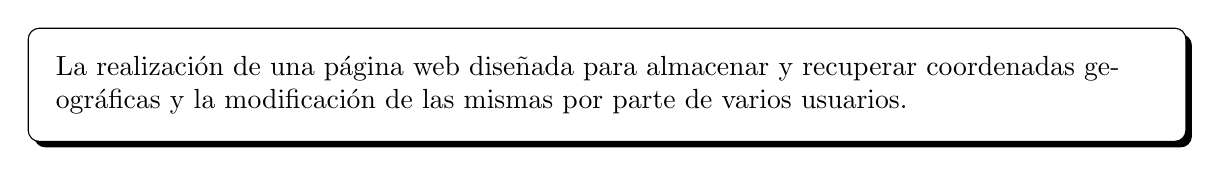
\begin{tikzpicture}
	\node[shadowBox] {La realización de una página web diseñada para almacenar y recuperar coordenadas geográficas y la modificación de las mismas por parte de varios usuarios.};
\end{tikzpicture}

El objetivo ha sido cumplido satisfactoriamente, logrando crear una herramienta web capaz de recuperar la posición geográfica del usuario, mostrar las ubicaciones guardadas por el mismo y permitir que otros usuarios modificasen las coordenadas de los objetos compartidos. Para marcar como terminado el objetivo principal del desarrollo se marcaron una serie de objetivos parciales, con el fin de asegurar la correcta finalización del trabajo. En la tabla \ref{tab:objetivos2} pueden verse estos objetivos y el momento en que adquirieron la consideración de terminados.

\begin{table}[hp]
  \centering 
  \rowcolors{1}{gray!25}{white}
  \begin{tabular}{p{0.2\linewidth}p{0.5\linewidth}p{0.2\linewidth}}
    \multicolumn{1}{l}{\cellcolor{black!30}\textbf{Id Objetivo}} & 
 	\multicolumn{1}{c}{\cellcolor{black!30}\textbf{Descripción del objetivo}}\\
 	\multicolumn{1}{c}{\cellcolor{black!30}\textbf{Consecución}}\\
    \toprule
    Objetivo 1 & Realizar una página web para el acceso a la herramienta & Sprint 1 \\
	Objetivo 2 & Añadir gestión de usuarios a la página (registro y control de acceso) & Sprint 1 \\
	Objetivo 3 & Permitir el almacenamiento, edición y recuperación de datos a través de la página web & Sprint 3 \\
	Objetivo 4 & Mostrar los datos almacenados mediante la inclusión de un mapa & Sprint 2 \\
	Objetivo 5 & Facilitar a un usuario permitir a otros usuarios la edición de los datos almacenados & Sprint 7\\
	Objetivo 6 & Añadir una opción para mostrar el recorrido desde el punto actual al punto almacenado Sprint 8\\
    \hline
  \end{tabular}
  \caption{Objetivos parciales del \ac{TFG}}
  \label{tab:objetivos2}
\end{table}

\subsection{Objetivo 1}
Se concluye este primer objetivo al término del Sprint 1, mediante la creación de un marco de trabajo en forma de página web que será la que de soporte a la totalidad de la herramienta.

\subsection{Objetivo 2}
Durante el primer Sprint también se da por concluido el segundo objetivo, ya que se dota al producto de una gestión básica de usuarios, permitiendo la creación, edición y eliminación de usuarios en el sistema.

\subsection{Objetivo 3}
La conclusión básica del objetivo se logra al término del tercer Sprint. Se habla de conlusión básica porque en este punto del desarrollo los usuarios únicamente tienen capacidad para almacenar los datos de un elemento. Al término del cuarto Sprint se le dota de la funcionalidad completa, en la que el usuario puede mantener tantos elementos como desee.

\subsection{Objetivo 4}
El objetivo cuatro se completa en el segundo Sprint, con la inclusión de un mapa interactivo en el que se muestran los datos almacenados y se termina de definir en el quinto Sprint, en el que, ante la existencia de varios elementos para mostrar, se añade la funcionalidad de mostrar sólo aquel que el usuario seleccione.

\subsection{Objetivo 5}
Al termino del séptimo Sprint, el objetivo queda satisfecho mediante la incorporación de las herramientas necesarias para conceder permiso a otros usuarios sobre los elementos que el usuario propietario así decida.

\subsection{Objetivo 6}
La consecución de todos los objetivos parciales se da al término del octavo sprint, cuando se muestra en el mapa interactivo una ruta a pie desde la ubicación del usuario hasta el elemento seleccionado.

\section{Propuestas de trabajo}
La herramienta mantiene varios aspectos que pueden ser mejorados. Estos posibles trabajos son:

\begin{itemize}[label={$\bullet$},labelindent=\parindent,leftmargin=2cm]
	\item Añadir autenticación mediante cuentas externas como Google, Facebook o Twitter.
	\item Añadir soporte para redes sociales
	\item Crear una herramienta móvil dedicada para los principales sistemas operativos móviles
	\item Permitir la creación y utilización de elementos de cualquier tipo, no restringiendo el uso únicamente a coches
	\item Permitir un cierto nivel de personalización en la forma de mostrar los datos en el mapa
\end{itemize}

\section{Recapitulación}
Durante el desarrollo del proyecto he conseguido alcanzar un conocimiento profundo de las tecnologías estudiadas, prácticamente todas ellas novedosas, y afianzar en los conceptos estudiados durante la carrera. El estudio de nuevos lenguajes de programación como Ruby on Rails o Javascript, la creación de interfaces adaptables a distintos sistemas, el aprendizaje de multitud de herramientas secundarias tan útiles y usadas en la vida diaria y la adquisición de nuevas competencias en la resolución de problemas de cierto alcance son objetivos nada desdeñables. \\
Durante la preparación de este proyecto he encontrado multitud de problemas a los que he tenido que encontrar respuesta de una u otra manera. La frustración ante fallos con aspecto de irresolubilidad y el aprendizaje de nuevas habilidades que me permitían superarlos, supone una lección extremadamente útil para mi futuro laboral, puesto que las tecnologías cambiarán con el paso del tiempo, pero las formas de enfrentarse a los problemas que surgirán durante su utilización no.

\hfill Juan Bausá Arpón

\hfill En Ciudad Real a 11 de enero de 2016

% Local Variables:
%  coding: utf-8
%  mode: latex
%  mode: flyspell
%  ispell-local-dictionary: "castellano8"
% End:

\appendix
\appendixtitle
\chapter{Ejemplo de anexo}

\blindtext

%{\scriptsize \chapter{GNU Free Documentation License}
\vspace{1.5cm}

Version 1.3, 3 November 2008

Copyright © 2000, 2001, 2002, 2007, 2008 Free Software Foundation,
Inc. <\url{http://fsf.org/}>

Everyone is permitted to copy and distribute verbatim copies of this
license document, but changing it is not allowed.


\setcounter{section}{-1}

\titleformat{\section}
  {\normalfont\normalsize\bfseries}{\arabic{section}.}{1em}{}

\section{PREAMBLE}

The purpose of this License is to make a manual, textbook, or other
functional and useful document ``free'' in the sense of freedom: to
assure everyone the effective freedom to copy and redistribute it,
with or without modifying it, either commercially or
noncommercially. Secondarily, this License preserves for the author
and publisher a way to get credit for their work, while not being
considered responsible for modifications made by others.

This License is a kind of ``copyleft'', which means that derivative
works of the document must themselves be free in the same sense. It
complements the GNU General Public License, which is a copyleft
license designed for free software.

We have designed this License in order to use it for manuals for free
software, because free software needs free documentation: a free
program should come with manuals providing the same freedoms that the
software does. But this License is not limited to software manuals; it
can be used for any textual work, regardless of subject matter or
whether it is published as a printed book. We recommend this License
principally for works whose purpose is instruction or reference.


\section{APPLICABILITY AND DEFINITIONS}

This License applies to any manual or other work, in any medium, that
contains a notice placed by the copyright holder saying it can be
distributed under the terms of this License. Such a notice grants a
world-wide, royalty-free license, unlimited in duration, to use that
work under the conditions stated herein. The ``Document'', below, refers
to any such manual or work. Any member of the public is a licensee,
and is addressed as ``you''. You accept the license if you copy, modify
or distribute the work in a way requiring permission under copyright
law.

A ``Modified Version'' of the Document means any work containing the
Document or a portion of it, either copied verbatim, or with
modifications and/or translated into another language.

A ``Secondary Section'' is a named appendix or a front-matter section of
the Document that deals exclusively with the relationship of the
publishers or authors of the Document to the Document's overall
subject (or to related matters) and contains nothing that could fall
directly within that overall subject. (Thus, if the Document is in
part a textbook of mathematics, a Secondary Section may not explain
any mathematics.) The relationship could be a matter of historical
connection with the subject or with related matters, or of legal,
commercial, philosophical, ethical or political position regarding
them.

The ``Invariant Sections'' are certain Secondary Sections whose titles
are designated, as being those of Invariant Sections, in the notice
that says that the Document is released under this License. If a
section does not fit the above definition of Secondary then it is not
allowed to be designated as Invariant. The Document may contain zero
Invariant Sections. If the Document does not identify any Invariant
Sections then there are none.

The ``Cover Texts'' are certain short passages of text that are listed,
as Front-Cover Texts or Back-Cover Texts, in the notice that says that
the Document is released under this License. A Front-Cover Text may be
at most 5 words, and a Back-Cover Text may be at most 25 words.

A ``Transparent'' copy of the Document means a machine-readable copy,
represented in a format whose specification is available to the
general public, that is suitable for revising the document
straightforwardly with generic text editors or (for images composed of
pixels) generic paint programs or (for drawings) some widely available
drawing editor, and that is suitable for input to text formatters or
for automatic translation to a variety of formats suitable for input
to text formatters. A copy made in an otherwise Transparent file
format whose markup, or absence of markup, has been arranged to thwart
or discourage subsequent modification by readers is not
Transparent. An image format is not Transparent if used for any
substantial amount of text. A copy that is not ``Transparent'' is called
``Opaque''.

Examples of suitable formats for Transparent copies include plain
ASCII without markup, Texinfo input format, LaTeX input format, SGML
or XML using a publicly available DTD, and standard-conforming simple
HTML, PostScript or PDF designed for human modification. Examples of
transparent image formats include PNG, XCF and JPG. Opaque formats
include proprietary formats that can be read and edited only by
proprietary word processors, SGML or XML for which the DTD and/or
processing tools are not generally available, and the
machine-generated HTML, PostScript or PDF produced by some word
processors for output purposes only.

The ``Title Page'' means, for a printed book, the title page itself,
plus such following pages as are needed to hold, legibly, the material
this License requires to appear in the title page. For works in
formats which do not have any title page as such, ``Title Page'' means
the text near the most prominent appearance of the work's title,
preceding the beginning of the body of the text.

The ``publisher'' means any person or entity that distributes copies of
the Document to the public.

A section ``Entitled XYZ'' means a named subunit of the Document whose
title either is precisely XYZ or contains XYZ in parentheses following
text that translates XYZ in another language. (Here XYZ stands for a
specific section name mentioned below, such as ``Acknowledgements'',
``Dedications'', ``Endorsements'', or ``History''.) To ``Preserve the Title''
of such a section when you modify the Document means that it remains a
section ``Entitled XYZ'' according to this definition.

The Document may include Warranty Disclaimers next to the notice which
states that this License applies to the Document. These Warranty
Disclaimers are considered to be included by reference in this
License, but only as regards disclaiming warranties: any other
implication that these Warranty Disclaimers may have is void and has
no effect on the meaning of this License.

\section{VERBATIM COPYING}

You may copy and distribute the Document in any medium, either
commercially or noncommercially, provided that this License, the
copyright notices, and the license notice saying this License applies
to the Document are reproduced in all copies, and that you add no
other conditions whatsoever to those of this License. You may not use
technical measures to obstruct or control the reading or further
copying of the copies you make or distribute. However, you may accept
compensation in exchange for copies. If you distribute a large enough
number of copies you must also follow the conditions in section 3.

You may also lend copies, under the same conditions stated above, and
you may publicly display copies.

\section{COPYING IN QUANTITY}

If you publish printed copies (or copies in media that commonly have
printed covers) of the Document, numbering more than 100, and the
Document's license notice requires Cover Texts, you must enclose the
copies in covers that carry, clearly and legibly, all these Cover
Texts: Front-Cover Texts on the front cover, and Back-Cover Texts on
the back cover. Both covers must also clearly and legibly identify you
as the publisher of these copies. The front cover must present the
full title with all words of the title equally prominent and
visible. You may add other material on the covers in addition. Copying
with changes limited to the covers, as long as they preserve the title
of the Document and satisfy these conditions, can be treated as
verbatim copying in other respects.

If the required texts for either cover are too voluminous to fit
legibly, you should put the first ones listed (as many as fit
reasonably) on the actual cover, and continue the rest onto adjacent
pages.

If you publish or distribute Opaque copies of the Document numbering
more than 100, you must either include a machine-readable Transparent
copy along with each Opaque copy, or state in or with each Opaque copy
a computer-network location from which the general network-using
public has access to download using public-standard network protocols
a complete Transparent copy of the Document, free of added
material. If you use the latter option, you must take reasonably
prudent steps, when you begin distribution of Opaque copies in
quantity, to ensure that this Transparent copy will remain thus
accessible at the stated location until at least one year after the
last time you distribute an Opaque copy (directly or through your
agents or retailers) of that edition to the public.

It is requested, but not required, that you contact the authors of the
Document well before redistributing any large number of copies, to
give them a chance to provide you with an updated version of the
Document.

\section{MODIFICATIONS}


You may copy and distribute a Modified Version of the Document under
the conditions of sections 2 and 3 above, provided that you release
the Modified Version under precisely this License, with the Modified
Version filling the role of the Document, thus licensing distribution
and modification of the Modified Version to whoever possesses a copy
of it. In addition, you must do these things in the Modified Version:


\begin{itemize}
\item A. Use in the Title Page (and on the covers, if any) a title
  distinct from that of the Document, and from those of previous
  versions (which should, if there were any, be listed in the History
  section of the Document). You may use the same title as a previous
  version if the original publisher of that version gives permission.

\item B. List on the Title Page, as authors, one or more persons or
  entities responsible for authorship of the modifications in the
  Modified Version, together with at least five of the principal
  authors of the Document (all of its principal authors, if it has
  fewer than five), unless they release you from this requirement.

\item C. State on the Title page the name of the publisher of the
  Modified Version, as the publisher.

\item D. Preserve all the copyright notices of the Document.

\item E. Add an appropriate copyright notice for your modifications
  adjacent to the other copyright notices.

\item F. Include, immediately after the copyright notices, a license
  notice giving the public permission to use the Modified Version
  under the terms of this License, in the form shown in the Addendum
  below.

\item G. Preserve in that license notice the full lists of Invariant
  Sections and required Cover Texts given in the Document's license
  notice.

\item H. Include an unaltered copy of this License.

\item I. Preserve the section Entitled ``History'', Preserve its Title,
  and add to it an item stating at least the title, year, new authors,
  and publisher of the Modified Version as given on the Title Page. If
  there is no section Entitled ``History'' in the Document, create one
  stating the title, year, authors, and publisher of the Document as
  given on its Title Page, then add an item describing the Modified
  Version as stated in the previous sentence.

\item J. Preserve the network location, if any, given in the Document
  for public access to a Transparent copy of the Document, and
  likewise the network locations given in the Document for previous
  versions it was based on. These may be placed in the ``History''
  section. You may omit a network location for a work that was
  published at least four years before the Document itself, or if the
  original publisher of the version it refers to gives permission.

\item K. For any section Entitled ``Acknowledgements'' or ``Dedications'',
  Preserve the Title of the section, and preserve in the section all
  the substance and tone of each of the contributor acknowledgements
  and/or dedications given therein.

\item L. Preserve all the Invariant Sections of the Document,
  unaltered in their text and in their titles. Section numbers or the
  equivalent are not considered part of the section titles.

\item M. Delete any section Entitled ``Endorsements''. Such a section
  may not be included in the Modified Version.

\item N. Do not retitle any existing section to be Entitled
  ``Endorsements'' or to conflict in title with any Invariant Section.

\item O. Preserve any Warranty Disclaimers.
\end{itemize}

If the Modified Version includes new front-matter sections or
appendices that qualify as Secondary Sections and contain no material
copied from the Document, you may at your option designate some or all
of these sections as invariant. To do this, add their titles to the
list of Invariant Sections in the Modified Version's license
notice. These titles must be distinct from any other section titles.

You may add a section Entitled ``Endorsements'', provided it contains
nothing but endorsements of your Modified Version by various
parties—for example, statements of peer review or that the text has
been approved by an organization as the authoritative definition of a
standard.

You may add a passage of up to five words as a Front-Cover Text, and a
passage of up to 25 words as a Back-Cover Text, to the end of the list
of Cover Texts in the Modified Version. Only one passage of
Front-Cover Text and one of Back-Cover Text may be added by (or
through arrangements made by) any one entity. If the Document already
includes a cover text for the same cover, previously added by you or
by arrangement made by the same entity you are acting on behalf of,
you may not add another; but you may replace the old one, on explicit
permission from the previous publisher that added the old one.

The author(s) and publisher(s) of the Document do not by this License
give permission to use their names for publicity for or to assert or
imply endorsement of any Modified Version.  5. COMBINING DOCUMENTS

You may combine the Document with other documents released under this
License, under the terms defined in section 4 above for modified
versions, provided that you include in the combination all of the
Invariant Sections of all of the original documents, unmodified, and
list them all as Invariant Sections of your combined work in its
license notice, and that you preserve all their Warranty Disclaimers.

The combined work need only contain one copy of this License, and
multiple identical Invariant Sections may be replaced with a single
copy. If there are multiple Invariant Sections with the same name but
different contents, make the title of each such section unique by
adding at the end of it, in parentheses, the name of the original
author or publisher of that section if known, or else a unique
number. Make the same adjustment to the section titles in the list of
Invariant Sections in the license notice of the combined work.

In the combination, you must combine any sections Entitled ``History''
in the various original documents, forming one section Entitled
``History''; likewise combine any sections Entitled ``Acknowledgements'',
and any sections Entitled ``Dedications''. You must delete all sections
Entitled ``Endorsements''.

\section{COLLECTIONS OF DOCUMENTS}


You may make a collection consisting of the Document and other
documents released under this License, and replace the individual
copies of this License in the various documents with a single copy
that is included in the collection, provided that you follow the rules
of this License for verbatim copying of each of the documents in all
other respects.

You may extract a single document from such a collection, and
distribute it individually under this License, provided you insert a
copy of this License into the extracted document, and follow this
License in all other respects regarding verbatim copying of that
document.


\section{AGGREGATION WITH INDEPENDENT WORKS}

A compilation of the Document or its derivatives with other separate
and independent documents or works, in or on a volume of a storage or
distribution medium, is called an ``aggregate'' if the copyright
resulting from the compilation is not used to limit the legal rights
of the compilation's users beyond what the individual works
permit. When the Document is included in an aggregate, this License
does not apply to the other works in the aggregate which are not
themselves derivative works of the Document.

If the Cover Text requirement of section 3 is applicable to these
copies of the Document, then if the Document is less than one half of
the entire aggregate, the Document's Cover Texts may be placed on
covers that bracket the Document within the aggregate, or the
electronic equivalent of covers if the Document is in electronic
form. Otherwise they must appear on printed covers that bracket the
whole aggregate.


\section{TRANSLATION}

Translation is considered a kind of modification, so you may
distribute translations of the Document under the terms of section
4. Replacing Invariant Sections with translations requires special
permission from their copyright holders, but you may include
translations of some or all Invariant Sections in addition to the
original versions of these Invariant Sections. You may include a
translation of this License, and all the license notices in the
Document, and any Warranty Disclaimers, provided that you also include
the original English version of this License and the original versions
of those notices and disclaimers. In case of a disagreement between
the translation and the original version of this License or a notice
or disclaimer, the original version will prevail.

If a section in the Document is Entitled ``Acknowledgements'',
``Dedications'', or ``History'', the requirement (section 4) to Preserve
its Title (section 1) will typically require changing the actual
title.


\section{TERMINATION}

You may not copy, modify, sublicense, or distribute the Document
except as expressly provided under this License. Any attempt otherwise
to copy, modify, sublicense, or distribute it is void, and will
automatically terminate your rights under this License.

However, if you cease all violation of this License, then your license
from a particular copyright holder is reinstated (a) provisionally,
unless and until the copyright holder explicitly and finally
terminates your license, and (b) permanently, if the copyright holder
fails to notify you of the violation by some reasonable means prior to
60 days after the cessation.

Moreover, your license from a particular copyright holder is
reinstated permanently if the copyright holder notifies you of the
violation by some reasonable means, this is the first time you have
received notice of violation of this License (for any work) from that
copyright holder, and you cure the violation prior to 30 days after
your receipt of the notice.

Termination of your rights under this section does not terminate the
licenses of parties who have received copies or rights from you under
this License. If your rights have been terminated and not permanently
reinstated, receipt of a copy of some or all of the same material does
not give you any rights to use it.


\section{FUTURE REVISIONS OF THIS LICENSE}

The Free Software Foundation may publish new, revised versions of the
GNU Free Documentation License from time to time. Such new versions
will be similar in spirit to the present version, but may differ in
detail to address new problems or concerns. See
http://www.gnu.org/copyleft/.

Each version of the License is given a distinguishing version
number. If the Document specifies that a particular numbered version
of this License ``or any later version'' applies to it, you have the
option of following the terms and conditions either of that specified
version or of any later version that has been published (not as a
draft) by the Free Software Foundation. If the Document does not
specify a version number of this License, you may choose any version
ever published (not as a draft) by the Free Software Foundation. If
the Document specifies that a proxy can decide which future versions
of this License can be used, that proxy's public statement of
acceptance of a version permanently authorizes you to choose that
version for the Document.


\section{RELICENSING}

``Massive Multiauthor Collaboration Site'' (or ``MMC Site'') means any
World Wide Web server that publishes copyrightable works and also
provides prominent facilities for anybody to edit those works. A
public wiki that anybody can edit is an example of such a server. A
``Massive Multiauthor Collaboration'' (or ``MMC'') contained in the site
means any set of copyrightable works thus published on the MMC site.

``CC-BY-SA'' means the Creative Commons Attribution-Share Alike 3.0
license published by Creative Commons Corporation, a not-for-profit
corporation with a principal place of business in San Francisco,
California, as well as future copyleft versions of that license
published by that same organization.

``Incorporate'' means to publish or republish a Document, in whole or in
part, as part of another Document.

An MMC is ``eligible for relicensing'' if it is licensed under this
License, and if all works that were first published under this License
somewhere other than this MMC, and subsequently incorporated in whole
or in part into the MMC, (1) had no cover texts or invariant sections,
and (2) were thus incorporated prior to November 1, 2008.

The operator of an MMC Site may republish an MMC contained in the site
under CC-BY-SA on the same site at any time before August 1, 2009,
provided the MMC is eligible for relicensing.
}


\backmatter
\bibliography{bibliography}
\cleardoublepage

\end{document}
